\documentclass[twoside]{book}

% Packages required by doxygen
\usepackage{fixltx2e}
\usepackage{calc}
\usepackage{doxygen}
\usepackage[export]{adjustbox} % also loads graphicx
\usepackage{graphicx}
\usepackage[utf8]{inputenc}
\usepackage{makeidx}
\usepackage{multicol}
\usepackage{multirow}
\PassOptionsToPackage{warn}{textcomp}
\usepackage{textcomp}
\usepackage[nointegrals]{wasysym}
\usepackage[table]{xcolor}

% Font selection
\usepackage[T1]{fontenc}
\usepackage[scaled=.90]{helvet}
\usepackage{courier}
\usepackage{amssymb}
\usepackage{sectsty}
\renewcommand{\familydefault}{\sfdefault}
\allsectionsfont{%
  \fontseries{bc}\selectfont%
  \color{darkgray}%
}
\renewcommand{\DoxyLabelFont}{%
  \fontseries{bc}\selectfont%
  \color{darkgray}%
}
\newcommand{\+}{\discretionary{\mbox{\scriptsize$\hookleftarrow$}}{}{}}

% Page & text layout
\usepackage{geometry}
\geometry{%
  a4paper,%
  top=2.5cm,%
  bottom=2.5cm,%
  left=2.5cm,%
  right=2.5cm%
}
\tolerance=750
\hfuzz=15pt
\hbadness=750
\setlength{\emergencystretch}{15pt}
\setlength{\parindent}{0cm}
\setlength{\parskip}{3ex plus 2ex minus 2ex}
\makeatletter
\renewcommand{\paragraph}{%
  \@startsection{paragraph}{4}{0ex}{-1.0ex}{1.0ex}{%
    \normalfont\normalsize\bfseries\SS@parafont%
  }%
}
\renewcommand{\subparagraph}{%
  \@startsection{subparagraph}{5}{0ex}{-1.0ex}{1.0ex}{%
    \normalfont\normalsize\bfseries\SS@subparafont%
  }%
}
\makeatother

% Headers & footers
\usepackage{fancyhdr}
\pagestyle{fancyplain}
\fancyhead[LE]{\fancyplain{}{\bfseries\thepage}}
\fancyhead[CE]{\fancyplain{}{}}
\fancyhead[RE]{\fancyplain{}{\bfseries\leftmark}}
\fancyhead[LO]{\fancyplain{}{\bfseries\rightmark}}
\fancyhead[CO]{\fancyplain{}{}}
\fancyhead[RO]{\fancyplain{}{\bfseries\thepage}}
\fancyfoot[LE]{\fancyplain{}{}}
\fancyfoot[CE]{\fancyplain{}{}}
\fancyfoot[RE]{\fancyplain{}{\bfseries\scriptsize Generated by Doxygen }}
\fancyfoot[LO]{\fancyplain{}{\bfseries\scriptsize Generated by Doxygen }}
\fancyfoot[CO]{\fancyplain{}{}}
\fancyfoot[RO]{\fancyplain{}{}}
\renewcommand{\footrulewidth}{0.4pt}
\renewcommand{\chaptermark}[1]{%
  \markboth{#1}{}%
}
\renewcommand{\sectionmark}[1]{%
  \markright{\thesection\ #1}%
}

% Indices & bibliography
\usepackage{natbib}
\usepackage[titles]{tocloft}
\setcounter{tocdepth}{3}
\setcounter{secnumdepth}{5}
\makeindex

% Hyperlinks (required, but should be loaded last)
\usepackage{ifpdf}
\ifpdf
  \usepackage[pdftex,pagebackref=true]{hyperref}
\else
  \usepackage[ps2pdf,pagebackref=true]{hyperref}
\fi
\hypersetup{%
  colorlinks=true,%
  linkcolor=blue,%
  citecolor=blue,%
  unicode%
}

% Custom commands
\newcommand{\clearemptydoublepage}{%
  \newpage{\pagestyle{empty}\cleardoublepage}%
}

\usepackage{caption}
\captionsetup{labelsep=space,justification=centering,font={bf},singlelinecheck=off,skip=4pt,position=top}

%===== C O N T E N T S =====

\begin{document}

% Titlepage & ToC
\hypersetup{pageanchor=false,
             bookmarksnumbered=true,
             pdfencoding=unicode
            }
\pagenumbering{alph}
\begin{titlepage}
\vspace*{7cm}
\begin{center}%
{\Large Gestro }\\
\vspace*{1cm}
{\large Generated by Doxygen 1.8.13}\\
\end{center}
\end{titlepage}
\clearemptydoublepage
\pagenumbering{roman}
\tableofcontents
\clearemptydoublepage
\pagenumbering{arabic}
\hypersetup{pageanchor=true}

%--- Begin generated contents ---
\chapter{Main Page}
\label{index}\hypertarget{index}{}Contents

\section*{\hyperlink{namespace_gestro}{Gestro}}

\href{https://github.com/RandomGuy-coder/Gestro}{\tt }

Controlling Linux system using hand gestures



     



$<$details open=\char`\"{}open\char`\"{}$>$


\begin{DoxyEnumerate}
\item \href{#About-Gestro}{\tt About Gestro} 
\begin{DoxyItemize}
\item \href{#Demonstration-Video}{\tt Demonstration Video} 
\item \href{#Features}{\tt Features} 
\item \href{#Built-With}{\tt Built With} 
\item \href{#Built-On}{\tt Built On} 
\end{DoxyItemize}
\item \href{#Getting-Started}{\tt Getting Started} 
\begin{DoxyItemize}
\item \href{#Prerequisites}{\tt Prerequisites} 
\item \href{#Installation-Guide}{\tt Installation Guide} 
\end{DoxyItemize}
\item \href{#Launching-Gestro}{\tt Launching Gestro} 
\begin{DoxyItemize}
\item \href{#Main-Program}{\tt Main Program} 
\item \href{#Unit-Tests}{\tt Unit Tests} 
\end{DoxyItemize}


\item \href{#Contributors}{\tt Contributors} 
\item \href{#Future-Enhancement}{\tt Future Enhancement} 
\item \href{#Social-Media}{\tt Social Media} 
\item \href{#Documentation}{\tt Documentation} 
\item \href{#License}{\tt License} 
\end{DoxyEnumerate}$<$/details$>$

\subsection*{About \hyperlink{namespace_gestro}{Gestro}}

\hyperlink{namespace_gestro}{Gestro} is developed by a group of students from The University of Glasgow currently undertaking the course of E\+N\+G5220 -\/ Real-\/time Embedded Systems under Team 26.

\hyperlink{namespace_gestro}{Gestro} is an application which allows users to control their Linux system using hand gestures so that users will be able to perform certains actions without the use of a keyboard and mouse. This is particularly useful in cases where users want to control their Linux PC while\+: being away from it, being unfamiliar with modern devices (such as Elderly people), et cetera.

By using a webcam and libraries such as Open\+CV, X11, et cetera, \hyperlink{namespace_gestro}{Gestro} is able to successfully translate hand gestures performed by users into commands that performs certain operations including, but not limited to, muting and unmuting the system\textquotesingle{}s volume, move window, mouse move and clicks. \hyperlink{namespace_gestro}{Gestro} is designed to be displayed using a Qt application on the users\textquotesingle{} Linux system running the Ubuntu distribution.

More details can be found below. However, for the complete information about \hyperlink{namespace_gestro}{Gestro}, please visit our \href{https://randomguy-coder.github.io/Gestro/}{\tt website}.

\subsubsection*{Demonstration Video}

Click to view our \mbox{[}demonstration video\mbox{]}()!

  

\subsubsection*{Features}


\begin{DoxyItemize}
\item Enter Spacebar (Used for Play and Pause).
\item Track mouse.
\item Perform mouse clicks.
\item Mute and Unmute Volume.
\item Move and Minimise window.
\end{DoxyItemize}

\subsubsection*{Built With}


\begin{DoxyItemize}
\item A PC running Ubuntu 18.\+04 L\+TS.
\item A webcam.
\end{DoxyItemize}

\subsubsection*{Built On}


\begin{DoxyItemize}
\item Iir
\item X11
\item Qt 5
\item C++
\item C\+Make
\item Open\+CV
\item Doxygen
\item libasound2-\/dev
\item Google Unit Test Framework
\end{DoxyItemize}

\subsection*{Getting Started}

\hyperlink{namespace_gestro}{Gestro} is designed to be used on Linux P\+Cs running the Ubuntu distribution. In particular, it was tested and found to be running perfectly on P\+Cs running Ubuntu 18.\+04 L\+TS.

\subsubsection*{Prerequisites}


\begin{DoxyItemize}
\item A PC running Ubuntu.
\item A webcam.
\end{DoxyItemize}

\hyperlink{namespace_gestro}{Gestro} requires the following tools and libraries to run (other versions are not tested)\+:
\begin{DoxyItemize}
\item X11
\item Qt 5
\item Open\+CV 4.\+5.\+5
\item libasound2-\/dev
\item Google Unit Test Frame\+Work
\end{DoxyItemize}

\begin{quote}
These required tools and libraries will be installed if you follow step 2 of the \href{#installation-guide}{\tt installation guide} below. \end{quote}


\subsubsection*{Installation Guide}

\begin{quote}
If permission is denied while trying to run any of the scripts, please enter the following Commands into the terminal and try running the script again, {\ttfamily sudo chmod +x $<$script\+\_\+name$>$.sh}. \end{quote}


\begin{quote}
For example, for the install\+\_\+dependencies.\+sh, enter {\ttfamily sudo chmod +x install\+\_\+dependencies.\+sh} into the terminal. \end{quote}


{\bfseries 1. Download the latest \mbox{[}release\mbox{]}() from our Github and extract the contents into the {\itshape Home} folder.}

\begin{quote}
Note\+: Make sure the folder with the contents is named \char`\"{}\+Gestro\char`\"{}. If not, rename it to \char`\"{}\+Gestro\char`\"{}. \end{quote}


\begin{quote}
Alternatively, launch a terminal and run\+: 
\begin{DoxyCode}
git clone https://github.com/RandomGuy-coder/Gestro.git
\end{DoxyCode}
 \end{quote}


{\bfseries 2. Launch a terminal and enter the following commands into it to install the requirements\+:} 
\begin{DoxyCode}
cd ~/Gestro && sudo ./install\_dependencies.sh
\end{DoxyCode}
 \begin{quote}
Note\+: If C\+Make version is found to be too low, please follow instructions \href{https://askubuntu.com/a/829311}{\tt here} to update C\+Make. After updating C\+Make, make sure to close and reopen the terminal before starting from step 2 again. \end{quote}


{\bfseries 3. Enter the following commands into the terminal to run the build script.} 
\begin{DoxyCode}
sudo ./build.sh
\end{DoxyCode}


\subsection*{Launching \hyperlink{namespace_gestro}{Gestro}}

Firstly, launch a terminal and enter the following commands to cd into the \hyperlink{namespace_gestro}{Gestro}\textquotesingle{}s bin directory\+: 
\begin{DoxyCode}
cd ~/Gestro/bin
\end{DoxyCode}


\subsubsection*{Main Program}

Start the \hyperlink{namespace_gestro}{Gestro} application by running the following commands\+:


\begin{DoxyCode}
./Gestro
\end{DoxyCode}
 {\bfseries For instructions on how to use the \hyperlink{namespace_gestro}{Gestro} application, please see \href{https://randomguy-coder.github.io/Gestro/user_manual.html}{\tt User Manual} on our \href{https://randomguy-coder.github.io/Gestro/}{\tt website}}.

\subsubsection*{Unit Tests}

Run the unit tests by running the following Commands\+: 
\begin{DoxyCode}
./test\_run
\end{DoxyCode}


\subsection*{Contributors\+:}

E\+N\+G5220 -\/ Real-\/time Embedded Systems -\/ Team 26\+:
\begin{DoxyItemize}
\item \href{https://github.com/RandomGuy-coder}{\tt Tushar Anil Mittal, 2669699M}
\item \href{https://github.com/terrsoshi}{\tt Tian Jie Wong, 2702282W}
\item \href{https://github.com/MuhatasimIntisar}{\tt Muhatasim Intisar, 2683935I}
\item \href{https://github.com/David2574}{\tt Ruoqi Sun, 2574212S}
\end{DoxyItemize}

\subsection*{Future Enhancement\+:}

Here are some of the planned features for this project\+:
\begin{DoxyItemize}
\item Enter other keys
\item Close Window
\item Change window size
\item Play Next and Previous
\item Zoom in and Zoom out
\item Switch between applications
\item Increase and Decrease Brightness
\end{DoxyItemize}

Propose for a new feature or report a bug \href{https://github.com/RandomGuy-coder/Gestro/issues}{\tt here}!

\begin{quote}
Feel free to contribute to this project by forking it and submitting a pull request for the added changes. \end{quote}


\subsection*{Social Media\+:}

$<$nav$>$ Follow us on\+:~\newline
~\newline
  \href{https://www.facebook.com/GestroProject}{\tt } \href{https://twitter.com/GestroProject}{\tt } \href{https://www.instagram.com/gestroproject/}{\tt } \href{https://hackaday.io/project/184728-gestro}{\tt }  $<$/nav$>$

\subsection*{Documentation}

Check out \href{https://randomguy-coder.github.io/Gestro/docs/html/index.html}{\tt Gestro\textquotesingle{}s documentation page}!

\subsection*{License}

Distributed under the G\+P\+L-\/3.\+0 License. See \href{https://github.com/RandomGuy-coder/Gestro/blob/main/LICENSE}{\tt {\ttfamily L\+I\+C\+E\+N\+SE}} for more information.

~\newline
 
\footnotesize {\itshape Copyright \copyright{} 2022; E\+N\+G5220 -\/ Real-\/\+Time-\/\+Embedded-\/\+Systems -\/ Team 26}
\normalsize ~\newline
 
\footnotesize {\itshape Distributed by a \href{https://github.com/RandomGuy-coder/Gestro/blob/main/LICENSE}{\tt G\+NU G\+P\+L-\/3.\+0 License.} }
\normalsize 
\chapter{Hierarchical Index}
\section{Class Hierarchy}
This inheritance list is sorted roughly, but not completely, alphabetically\+:\begin{DoxyCompactList}
\item \contentsline{section}{Gesture\+Detection\+:\+:Capture}{\pageref{class_gesture_detection_1_1_capture}}{}
\item \contentsline{section}{Gestro\+:\+:Capture\+And\+Detect\+Callback\+Interface}{\pageref{class_gestro_1_1_capture_and_detect_callback_interface}}{}
\begin{DoxyCompactList}
\item \contentsline{section}{Gestro\+:\+:Capture\+And\+Detect}{\pageref{class_gestro_1_1_capture_and_detect}}{}
\end{DoxyCompactList}
\item \contentsline{section}{Controller\+Screen\+Callback\+Interface}{\pageref{class_controller_screen_callback_interface}}{}
\begin{DoxyCompactList}
\item \contentsline{section}{Controller\+Screen}{\pageref{class_controller_screen}}{}
\end{DoxyCompactList}
\item \contentsline{section}{Custom\+Signals}{\pageref{struct_custom_signals}}{}
\item \contentsline{section}{Gestro\+:\+:Display\+Control\+Callback\+Interface}{\pageref{class_gestro_1_1_display_control_callback_interface}}{}
\begin{DoxyCompactList}
\item \contentsline{section}{Gestro\+:\+:Display\+Control}{\pageref{class_gestro_1_1_display_control}}{}
\end{DoxyCompactList}
\item \contentsline{section}{Gesture\+Detection\+:\+:Enabled\+Command}{\pageref{class_gesture_detection_1_1_enabled_command}}{}
\item \contentsline{section}{Gesture\+Detection\+:\+:Finger\+And\+Coordinates}{\pageref{class_gesture_detection_1_1_finger_and_coordinates}}{}
\item \contentsline{section}{Gesture\+Detection\+:\+:Finger\+Counter}{\pageref{class_gesture_detection_1_1_finger_counter}}{}
\item \contentsline{section}{Ubuntu\+Controller\+:\+:Keyboard\+Action}{\pageref{class_ubuntu_controller_1_1_keyboard_action}}{}
\begin{DoxyCompactList}
\item \contentsline{section}{Gestro\+:\+:Display\+Control}{\pageref{class_gestro_1_1_display_control}}{}
\end{DoxyCompactList}
\item \contentsline{section}{Ubuntu\+Controller\+:\+:Keyboard\+Event}{\pageref{class_ubuntu_controller_1_1_keyboard_event}}{}
\item \contentsline{section}{Ubuntu\+Controller\+:\+:Mouse\+Action}{\pageref{class_ubuntu_controller_1_1_mouse_action}}{}
\begin{DoxyCompactList}
\item \contentsline{section}{Gestro\+:\+:Display\+Control}{\pageref{class_gestro_1_1_display_control}}{}
\end{DoxyCompactList}
\item \contentsline{section}{Ubuntu\+Controller\+:\+:Mouse\+Control}{\pageref{class_ubuntu_controller_1_1_mouse_control}}{}
\item Q\+Dialog\begin{DoxyCompactList}
\item \contentsline{section}{Controller\+Screen}{\pageref{class_controller_screen}}{}
\end{DoxyCompactList}
\item Q\+Widget\begin{DoxyCompactList}
\item \contentsline{section}{Start\+Screen}{\pageref{class_start_screen}}{}
\end{DoxyCompactList}
\item \contentsline{section}{Gesture\+Detection\+:\+:Skin\+Color\+Detector}{\pageref{class_gesture_detection_1_1_skin_color_detector}}{}
\item \contentsline{section}{Ubuntu\+Controller\+:\+:Volume\+Control}{\pageref{class_ubuntu_controller_1_1_volume_control}}{}
\begin{DoxyCompactList}
\item \contentsline{section}{Gestro\+:\+:Display\+Control}{\pageref{class_gestro_1_1_display_control}}{}
\end{DoxyCompactList}
\item \contentsline{section}{Ubuntu\+Controller\+:\+:Window\+Action}{\pageref{class_ubuntu_controller_1_1_window_action}}{}
\begin{DoxyCompactList}
\item \contentsline{section}{Gestro\+:\+:Display\+Control}{\pageref{class_gestro_1_1_display_control}}{}
\end{DoxyCompactList}
\item \contentsline{section}{Ubuntu\+Controller\+:\+:Window\+Control}{\pageref{class_ubuntu_controller_1_1_window_control}}{}
\end{DoxyCompactList}

\chapter{Class Index}
\doxysection{Class List}
Here are the classes, structs, unions and interfaces with brief descriptions\+:\begin{DoxyCompactList}
\item\contentsline{section}{\mbox{\hyperlink{classkeyboard__event}{keyboard\+\_\+event}} }{\pageref{classkeyboard__event}}{}
\item\contentsline{section}{\mbox{\hyperlink{classkeyboard_action}{keyboard\+Action}} }{\pageref{classkeyboard_action}}{}
\item\contentsline{section}{\mbox{\hyperlink{classmouse__control}{mouse\+\_\+control}} }{\pageref{classmouse__control}}{}
\item\contentsline{section}{\mbox{\hyperlink{classmouse_action}{mouse\+Action}} }{\pageref{classmouse_action}}{}
\item\contentsline{section}{\mbox{\hyperlink{classvolume_control}{volume\+Control}} }{\pageref{classvolume_control}}{}
\item\contentsline{section}{\mbox{\hyperlink{classwindow__control}{window\+\_\+control}} }{\pageref{classwindow__control}}{}
\item\contentsline{section}{\mbox{\hyperlink{classwindow_action}{window\+Action}} }{\pageref{classwindow_action}}{}
\end{DoxyCompactList}

\chapter{File Index}
\section{File List}
Here is a list of all files with brief descriptions\+:\begin{DoxyCompactList}
\item\contentsline{section}{src/\hyperlink{main_8cpp}{main.\+cpp} }{\pageref{main_8cpp}}{}
\item\contentsline{section}{src/gesture\+\_\+detection/\hyperlink{_capture_8cpp}{Capture.\+cpp} }{\pageref{_capture_8cpp}}{}
\item\contentsline{section}{src/gesture\+\_\+detection/\hyperlink{_capture_8h}{Capture.\+h} }{\pageref{_capture_8h}}{}
\item\contentsline{section}{src/gesture\+\_\+detection/\hyperlink{_capture_and_detect_8cpp}{Capture\+And\+Detect.\+cpp} }{\pageref{_capture_and_detect_8cpp}}{}
\item\contentsline{section}{src/gesture\+\_\+detection/\hyperlink{_capture_and_detect_8h}{Capture\+And\+Detect.\+h} }{\pageref{_capture_and_detect_8h}}{}
\item\contentsline{section}{src/gesture\+\_\+detection/\hyperlink{_capture_and_detect_callback_interface_8h}{Capture\+And\+Detect\+Callback\+Interface.\+h} }{\pageref{_capture_and_detect_callback_interface_8h}}{}
\item\contentsline{section}{src/gesture\+\_\+detection/\hyperlink{_commands_8cpp}{Commands.\+cpp} }{\pageref{_commands_8cpp}}{}
\item\contentsline{section}{src/gesture\+\_\+detection/\hyperlink{_commands_8h}{Commands.\+h} }{\pageref{_commands_8h}}{}
\item\contentsline{section}{src/gesture\+\_\+detection/\hyperlink{_finger_and_coordinates_8cpp}{Finger\+And\+Coordinates.\+cpp} }{\pageref{_finger_and_coordinates_8cpp}}{}
\item\contentsline{section}{src/gesture\+\_\+detection/\hyperlink{_finger_and_coordinates_8h}{Finger\+And\+Coordinates.\+h} }{\pageref{_finger_and_coordinates_8h}}{}
\item\contentsline{section}{src/gesture\+\_\+detection/\hyperlink{_finger_counter_8cpp}{Finger\+Counter.\+cpp} }{\pageref{_finger_counter_8cpp}}{}
\item\contentsline{section}{src/gesture\+\_\+detection/\hyperlink{_finger_counter_8h}{Finger\+Counter.\+h} }{\pageref{_finger_counter_8h}}{}
\item\contentsline{section}{src/gesture\+\_\+detection/\hyperlink{_skin_color_detector_8cpp}{Skin\+Color\+Detector.\+cpp} }{\pageref{_skin_color_detector_8cpp}}{}
\item\contentsline{section}{src/gesture\+\_\+detection/\hyperlink{_skin_color_detector_8h}{Skin\+Color\+Detector.\+h} }{\pageref{_skin_color_detector_8h}}{}
\item\contentsline{section}{src/gui/\hyperlink{_controller_screen_8cpp}{Controller\+Screen.\+cpp} }{\pageref{_controller_screen_8cpp}}{}
\item\contentsline{section}{src/gui/\hyperlink{_controller_screen_8h}{Controller\+Screen.\+h} }{\pageref{_controller_screen_8h}}{}
\item\contentsline{section}{src/gui/\hyperlink{_controller_screen_callback_interface_8h}{Controller\+Screen\+Callback\+Interface.\+h} }{\pageref{_controller_screen_callback_interface_8h}}{}
\item\contentsline{section}{src/gui/\hyperlink{_custom_signals_8h}{Custom\+Signals.\+h} }{\pageref{_custom_signals_8h}}{}
\item\contentsline{section}{src/gui/\hyperlink{_start_screen_8cpp}{Start\+Screen.\+cpp} }{\pageref{_start_screen_8cpp}}{}
\item\contentsline{section}{src/gui/\hyperlink{_start_screen_8h}{Start\+Screen.\+h} }{\pageref{_start_screen_8h}}{}
\item\contentsline{section}{src/ubuntu\+\_\+controls/\hyperlink{_display_control_8cpp}{Display\+Control.\+cpp} }{\pageref{_display_control_8cpp}}{}
\item\contentsline{section}{src/ubuntu\+\_\+controls/\hyperlink{_display_control_8h}{Display\+Control.\+h} }{\pageref{_display_control_8h}}{}
\item\contentsline{section}{src/ubuntu\+\_\+controls/\hyperlink{_display_control_callback_interface_8h}{Display\+Control\+Callback\+Interface.\+h} }{\pageref{_display_control_callback_interface_8h}}{}
\item\contentsline{section}{src/ubuntu\+\_\+controls/\hyperlink{_keyboard_action_8cpp}{Keyboard\+Action.\+cpp} }{\pageref{_keyboard_action_8cpp}}{}
\item\contentsline{section}{src/ubuntu\+\_\+controls/\hyperlink{_keyboard_action_8h}{Keyboard\+Action.\+h} }{\pageref{_keyboard_action_8h}}{}
\item\contentsline{section}{src/ubuntu\+\_\+controls/\hyperlink{_keyboard_event_8cpp}{Keyboard\+Event.\+cpp} }{\pageref{_keyboard_event_8cpp}}{}
\item\contentsline{section}{src/ubuntu\+\_\+controls/\hyperlink{_keyboard_event_8h}{Keyboard\+Event.\+h} }{\pageref{_keyboard_event_8h}}{}
\item\contentsline{section}{src/ubuntu\+\_\+controls/\hyperlink{_mouse_action_8cpp}{Mouse\+Action.\+cpp} }{\pageref{_mouse_action_8cpp}}{}
\item\contentsline{section}{src/ubuntu\+\_\+controls/\hyperlink{_mouse_action_8h}{Mouse\+Action.\+h} }{\pageref{_mouse_action_8h}}{}
\item\contentsline{section}{src/ubuntu\+\_\+controls/\hyperlink{_mouse_control_8cpp}{Mouse\+Control.\+cpp} }{\pageref{_mouse_control_8cpp}}{}
\item\contentsline{section}{src/ubuntu\+\_\+controls/\hyperlink{_mouse_control_8h}{Mouse\+Control.\+h} }{\pageref{_mouse_control_8h}}{}
\item\contentsline{section}{src/ubuntu\+\_\+controls/\hyperlink{_volume_control_8cpp}{Volume\+Control.\+cpp} }{\pageref{_volume_control_8cpp}}{}
\item\contentsline{section}{src/ubuntu\+\_\+controls/\hyperlink{_volume_control_8h}{Volume\+Control.\+h} }{\pageref{_volume_control_8h}}{}
\item\contentsline{section}{src/ubuntu\+\_\+controls/\hyperlink{_window_action_8cpp}{Window\+Action.\+cpp} }{\pageref{_window_action_8cpp}}{}
\item\contentsline{section}{src/ubuntu\+\_\+controls/\hyperlink{_window_action_8h}{Window\+Action.\+h} }{\pageref{_window_action_8h}}{}
\item\contentsline{section}{src/ubuntu\+\_\+controls/\hyperlink{_window_control_8cpp}{Window\+Control.\+cpp} }{\pageref{_window_control_8cpp}}{}
\item\contentsline{section}{src/ubuntu\+\_\+controls/\hyperlink{_window_control_8h}{Window\+Control.\+h} }{\pageref{_window_control_8h}}{}
\end{DoxyCompactList}

\chapter{Class Documentation}
\hypertarget{classCapture}{}\section{Capture Class Reference}
\label{classCapture}\index{Capture@{Capture}}


{\ttfamily \#include $<$Capture.\+h$>$}

\subsection*{Public Member Functions}
\begin{DoxyCompactItemize}
\item 
\hyperlink{classCapture_a97036b5d271238bd4852da79a0091b57}{Capture} ()
\item 
void \hyperlink{classCapture_a1c661ca1dca730fae534cb8f54ff6ef5}{init} (\hyperlink{classCaptureAndDetectCallbackInterface}{Capture\+And\+Detect\+Callback\+Interface} $\ast$, int, int)
\item 
void \hyperlink{classCapture_a2ffe4eeac4caa296f4fcc75cc82c1436}{start} ()
\item 
void \hyperlink{classCapture_ab632f1927461a909b18cce71ec96f76d}{stop} ()
\end{DoxyCompactItemize}
\subsection*{Public Attributes}
\begin{DoxyCompactItemize}
\item 
bool \hyperlink{classCapture_a4120483ac2f664e14a80ec5dcd9915cb}{running} = false
\begin{DoxyCompactList}\small\item\em boolean to check if cmaera is running \end{DoxyCompactList}\end{DoxyCompactItemize}


\subsection{Detailed Description}
A class that captures images from the webcam and calls the callback function with the image. 

\subsection{Constructor \& Destructor Documentation}
\mbox{\Hypertarget{classCapture_a97036b5d271238bd4852da79a0091b57}\label{classCapture_a97036b5d271238bd4852da79a0091b57}} 
\index{Capture@{Capture}!Capture@{Capture}}
\index{Capture@{Capture}!Capture@{Capture}}
\subsubsection{\texorpdfstring{Capture()}{Capture()}}
{\footnotesize\ttfamily Capture\+::\+Capture (\begin{DoxyParamCaption}{ }\end{DoxyParamCaption})}

The constructor for the class. 

\subsection{Member Function Documentation}
\mbox{\Hypertarget{classCapture_a1c661ca1dca730fae534cb8f54ff6ef5}\label{classCapture_a1c661ca1dca730fae534cb8f54ff6ef5}} 
\index{Capture@{Capture}!init@{init}}
\index{init@{init}!Capture@{Capture}}
\subsubsection{\texorpdfstring{init()}{init()}}
{\footnotesize\ttfamily void Capture\+::init (\begin{DoxyParamCaption}\item[{\hyperlink{classCaptureAndDetectCallbackInterface}{Capture\+And\+Detect\+Callback\+Interface} $\ast$}]{interface,  }\item[{int}]{width,  }\item[{int}]{height }\end{DoxyParamCaption})}

It initializes the \hyperlink{classCapture}{Capture} class with the width and height of the image to be captured, and a pointer to the Detect\+Interface class


\begin{DoxyParams}{Parameters}
{\em interface} & The interface that will be called when a new frame is available. \\
\hline
{\em width} & The width of the image to be captured. \\
\hline
{\em height} & The height of the image to be captured. \\
\hline
\end{DoxyParams}
\mbox{\Hypertarget{classCapture_a2ffe4eeac4caa296f4fcc75cc82c1436}\label{classCapture_a2ffe4eeac4caa296f4fcc75cc82c1436}} 
\index{Capture@{Capture}!start@{start}}
\index{start@{start}!Capture@{Capture}}
\subsubsection{\texorpdfstring{start()}{start()}}
{\footnotesize\ttfamily void Capture\+::start (\begin{DoxyParamCaption}{ }\end{DoxyParamCaption})}

It starts a thread that runs the image\+Cap function to read Images \mbox{\Hypertarget{classCapture_ab632f1927461a909b18cce71ec96f76d}\label{classCapture_ab632f1927461a909b18cce71ec96f76d}} 
\index{Capture@{Capture}!stop@{stop}}
\index{stop@{stop}!Capture@{Capture}}
\subsubsection{\texorpdfstring{stop()}{stop()}}
{\footnotesize\ttfamily void Capture\+::stop (\begin{DoxyParamCaption}{ }\end{DoxyParamCaption})}

It stops the capture thread by setting the running flag to false, and then waits for the thread to finish 

\subsection{Member Data Documentation}
\mbox{\Hypertarget{classCapture_a4120483ac2f664e14a80ec5dcd9915cb}\label{classCapture_a4120483ac2f664e14a80ec5dcd9915cb}} 
\index{Capture@{Capture}!running@{running}}
\index{running@{running}!Capture@{Capture}}
\subsubsection{\texorpdfstring{running}{running}}
{\footnotesize\ttfamily bool Capture\+::running = false}



boolean to check if cmaera is running 



The documentation for this class was generated from the following files\+:\begin{DoxyCompactItemize}
\item 
src/gesture\+\_\+detection/\hyperlink{Capture_8h}{Capture.\+h}\item 
src/gesture\+\_\+detection/\hyperlink{Capture_8cpp}{Capture.\+cpp}\end{DoxyCompactItemize}

\hypertarget{classCaptureAndDetect}{}\section{Capture\+And\+Detect Class Reference}
\label{classCaptureAndDetect}\index{Capture\+And\+Detect@{Capture\+And\+Detect}}


This class takes care of starting threads to capture image, process and publish commands.  




{\ttfamily \#include $<$Capture\+And\+Detect.\+h$>$}



Inheritance diagram for Capture\+And\+Detect\+:\nopagebreak
\begin{figure}[H]
\begin{center}
\leavevmode
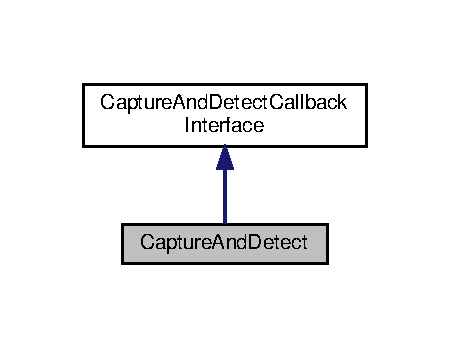
\includegraphics[width=216pt]{classCaptureAndDetect__inherit__graph}
\end{center}
\end{figure}


Collaboration diagram for Capture\+And\+Detect\+:\nopagebreak
\begin{figure}[H]
\begin{center}
\leavevmode
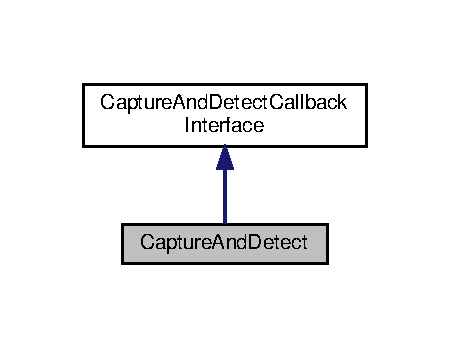
\includegraphics[width=216pt]{classCaptureAndDetect__coll__graph}
\end{center}
\end{figure}
\subsection*{Public Member Functions}
\begin{DoxyCompactItemize}
\item 
\hyperlink{classCaptureAndDetect_a26c41eaa5100975ec0f50c97592f4bf1}{Capture\+And\+Detect} ()
\item 
void \hyperlink{classCaptureAndDetect_a485523d1c8231e2f744bf9d7fa110f88}{init} (Controller\+Screen\+Callback\+Interface $\ast$, int, int, \hyperlink{CaptureAndDetect_8h_a3c1fc1369ee351f25804c8cde5e85ac3}{Resolution} width=\hyperlink{CaptureAndDetect_8h_a3c1fc1369ee351f25804c8cde5e85ac3a278580710dc7c233b4035c222f100b9f}{W\+I\+D\+T\+H\+\_\+1280}, \hyperlink{CaptureAndDetect_8h_a3c1fc1369ee351f25804c8cde5e85ac3}{Resolution} height=\hyperlink{CaptureAndDetect_8h_a3c1fc1369ee351f25804c8cde5e85ac3aaf8940bab7f04c8cd702f61c4d051f27}{H\+E\+I\+G\+H\+T\+\_\+720})
\item 
void \hyperlink{classCaptureAndDetect_aafb4f601f860dd38f514f6dd29a1d016}{calibrate\+Values} (int, int, int, int)
\item 
void \hyperlink{classCaptureAndDetect_a7f18d1c58b2ae4241766b36aa27385e9}{new\+Frame} (Mat) override
\item 
void \hyperlink{classCaptureAndDetect_ac60f9b1d192c043fa9b40c38fc5599e6}{calibrate\+Color\+Pressed} ()
\item 
void \hyperlink{classCaptureAndDetect_a53065abfb6eed6c074ad4d3370b3f232}{calibrate\+Background\+Remover} ()
\item 
void \hyperlink{classCaptureAndDetect_a3f1ba69514a2debbc6b2a03e76f31b65}{display\+Image} (int)
\item 
void \hyperlink{classCaptureAndDetect_aa75e3ba836797d18aa02c72bbf975082}{connect\+Control\+Callback} (Display\+Control\+Callback\+Interface $\ast$)
\item 
void \hyperlink{classCaptureAndDetect_ac7e70bbcade4e0023541c556ee7cb34e}{process\+Frame} ()
\item 
bool \hyperlink{classCaptureAndDetect_a1620075ba1bf4d52a4e455c20f7ac3d1}{check\+For\+Palm} ()
\item 
void \hyperlink{classCaptureAndDetect_af376ab5418f7b235ee181d574da71fd6}{add\+To\+Buffer} (\hyperlink{classFingerAndCoordinates}{Finger\+And\+Coordinates}) override
\end{DoxyCompactItemize}
\subsection*{Public Attributes}
\begin{DoxyCompactItemize}
\item 
bool \hyperlink{classCaptureAndDetect_ae57b827ebac2b4d5f5baaa8935442183}{calibrate} = false
\item 
Mat \hyperlink{classCaptureAndDetect_ad614571fedee59ecccccf0c14c3dd542}{recieved\+Frame}
\begin{DoxyCompactList}\small\item\em frame received from capture thread \end{DoxyCompactList}\end{DoxyCompactItemize}


\subsection{Detailed Description}
This class takes care of starting threads to capture image, process and publish commands. 

This class is the mediator between the different functions of the application. Connecting between image capturing, G\+UI and and Display\+Control to publish the detected commands. 

\subsection{Constructor \& Destructor Documentation}
\mbox{\Hypertarget{classCaptureAndDetect_a26c41eaa5100975ec0f50c97592f4bf1}\label{classCaptureAndDetect_a26c41eaa5100975ec0f50c97592f4bf1}} 
\index{Capture\+And\+Detect@{Capture\+And\+Detect}!Capture\+And\+Detect@{Capture\+And\+Detect}}
\index{Capture\+And\+Detect@{Capture\+And\+Detect}!Capture\+And\+Detect@{Capture\+And\+Detect}}
\subsubsection{\texorpdfstring{Capture\+And\+Detect()}{CaptureAndDetect()}}
{\footnotesize\ttfamily Capture\+And\+Detect\+::\+Capture\+And\+Detect (\begin{DoxyParamCaption}{ }\end{DoxyParamCaption})}

The constructor for the \hyperlink{classCaptureAndDetect}{Capture\+And\+Detect} class. 

\subsection{Member Function Documentation}
\mbox{\Hypertarget{classCaptureAndDetect_af376ab5418f7b235ee181d574da71fd6}\label{classCaptureAndDetect_af376ab5418f7b235ee181d574da71fd6}} 
\index{Capture\+And\+Detect@{Capture\+And\+Detect}!add\+To\+Buffer@{add\+To\+Buffer}}
\index{add\+To\+Buffer@{add\+To\+Buffer}!Capture\+And\+Detect@{Capture\+And\+Detect}}
\subsubsection{\texorpdfstring{add\+To\+Buffer()}{addToBuffer()}}
{\footnotesize\ttfamily void Capture\+And\+Detect\+::add\+To\+Buffer (\begin{DoxyParamCaption}\item[{\hyperlink{classFingerAndCoordinates}{Finger\+And\+Coordinates}}]{finger }\end{DoxyParamCaption})\hspace{0.3cm}{\ttfamily [override]}, {\ttfamily [virtual]}}

It adds a finger to the buffer


\begin{DoxyParams}{Parameters}
{\em finger} & The finger that was detected. \\
\hline
\end{DoxyParams}


Implements \hyperlink{classCaptureAndDetectCallbackInterface_a259dc71fd5d02424b91906d708e7de1f}{Capture\+And\+Detect\+Callback\+Interface}.

\mbox{\Hypertarget{classCaptureAndDetect_a53065abfb6eed6c074ad4d3370b3f232}\label{classCaptureAndDetect_a53065abfb6eed6c074ad4d3370b3f232}} 
\index{Capture\+And\+Detect@{Capture\+And\+Detect}!calibrate\+Background\+Remover@{calibrate\+Background\+Remover}}
\index{calibrate\+Background\+Remover@{calibrate\+Background\+Remover}!Capture\+And\+Detect@{Capture\+And\+Detect}}
\subsubsection{\texorpdfstring{calibrate\+Background\+Remover()}{calibrateBackgroundRemover()}}
{\footnotesize\ttfamily void Capture\+And\+Detect\+::calibrate\+Background\+Remover (\begin{DoxyParamCaption}{ }\end{DoxyParamCaption})}

It creates a background remover object that will be used to remove the background from the video frames \mbox{\Hypertarget{classCaptureAndDetect_ac60f9b1d192c043fa9b40c38fc5599e6}\label{classCaptureAndDetect_ac60f9b1d192c043fa9b40c38fc5599e6}} 
\index{Capture\+And\+Detect@{Capture\+And\+Detect}!calibrate\+Color\+Pressed@{calibrate\+Color\+Pressed}}
\index{calibrate\+Color\+Pressed@{calibrate\+Color\+Pressed}!Capture\+And\+Detect@{Capture\+And\+Detect}}
\subsubsection{\texorpdfstring{calibrate\+Color\+Pressed()}{calibrateColorPressed()}}
{\footnotesize\ttfamily void Capture\+And\+Detect\+::calibrate\+Color\+Pressed (\begin{DoxyParamCaption}{ }\end{DoxyParamCaption})}

It calls the calibrate function of the skin\+Detector object, which returns a vector of 4 integers, which are then passed to the callback function update\+Calibrated\+Trackbar, which updates the trackbar values \mbox{\Hypertarget{classCaptureAndDetect_aafb4f601f860dd38f514f6dd29a1d016}\label{classCaptureAndDetect_aafb4f601f860dd38f514f6dd29a1d016}} 
\index{Capture\+And\+Detect@{Capture\+And\+Detect}!calibrate\+Values@{calibrate\+Values}}
\index{calibrate\+Values@{calibrate\+Values}!Capture\+And\+Detect@{Capture\+And\+Detect}}
\subsubsection{\texorpdfstring{calibrate\+Values()}{calibrateValues()}}
{\footnotesize\ttfamily void Capture\+And\+Detect\+::calibrate\+Values (\begin{DoxyParamCaption}\item[{int}]{h\+Min,  }\item[{int}]{h\+Max,  }\item[{int}]{s\+Min,  }\item[{int}]{s\+Max }\end{DoxyParamCaption})}

It takes in the minimum and maximum values for the hue and saturation channels, and then passes them to the skin\+Detector object\textquotesingle{}s \hyperlink{classCaptureAndDetect_aafb4f601f860dd38f514f6dd29a1d016}{calibrate\+Values()} function


\begin{DoxyParams}{Parameters}
{\em h\+Min} & Minimum Hue value \\
\hline
{\em h\+Max} & The maximum hue value for the skin color. \\
\hline
{\em s\+Min} & Minimum saturation value for the skin color. \\
\hline
{\em s\+Max} & The maximum saturation value for the skin color. \\
\hline
\end{DoxyParams}
\mbox{\Hypertarget{classCaptureAndDetect_a1620075ba1bf4d52a4e455c20f7ac3d1}\label{classCaptureAndDetect_a1620075ba1bf4d52a4e455c20f7ac3d1}} 
\index{Capture\+And\+Detect@{Capture\+And\+Detect}!check\+For\+Palm@{check\+For\+Palm}}
\index{check\+For\+Palm@{check\+For\+Palm}!Capture\+And\+Detect@{Capture\+And\+Detect}}
\subsubsection{\texorpdfstring{check\+For\+Palm()}{checkForPalm()}}
{\footnotesize\ttfamily bool Capture\+And\+Detect\+::check\+For\+Palm (\begin{DoxyParamCaption}{ }\end{DoxyParamCaption})\hspace{0.3cm}{\ttfamily [virtual]}}

It takes the current frame, and checks to see if there is a palm in it

\begin{DoxyReturn}{Returns}
A boolean value. 
\end{DoxyReturn}


Implements \hyperlink{classCaptureAndDetectCallbackInterface_a64755838dd5592bae3ca06b4c5a0d72f}{Capture\+And\+Detect\+Callback\+Interface}.

\mbox{\Hypertarget{classCaptureAndDetect_aa75e3ba836797d18aa02c72bbf975082}\label{classCaptureAndDetect_aa75e3ba836797d18aa02c72bbf975082}} 
\index{Capture\+And\+Detect@{Capture\+And\+Detect}!connect\+Control\+Callback@{connect\+Control\+Callback}}
\index{connect\+Control\+Callback@{connect\+Control\+Callback}!Capture\+And\+Detect@{Capture\+And\+Detect}}
\subsubsection{\texorpdfstring{connect\+Control\+Callback()}{connectControlCallback()}}
{\footnotesize\ttfamily void Capture\+And\+Detect\+::connect\+Control\+Callback (\begin{DoxyParamCaption}\item[{Display\+Control\+Callback\+Interface $\ast$}]{interface }\end{DoxyParamCaption})}

This function is called by the Display\+Control class to connect the \hyperlink{classCaptureAndDetect}{Capture\+And\+Detect} class to the Display\+Control class.


\begin{DoxyParams}{Parameters}
{\em interface} & The interface that will be used to communicate with the display control. \\
\hline
\end{DoxyParams}
\mbox{\Hypertarget{classCaptureAndDetect_a3f1ba69514a2debbc6b2a03e76f31b65}\label{classCaptureAndDetect_a3f1ba69514a2debbc6b2a03e76f31b65}} 
\index{Capture\+And\+Detect@{Capture\+And\+Detect}!display\+Image@{display\+Image}}
\index{display\+Image@{display\+Image}!Capture\+And\+Detect@{Capture\+And\+Detect}}
\subsubsection{\texorpdfstring{display\+Image()}{displayImage()}}
{\footnotesize\ttfamily void Capture\+And\+Detect\+::display\+Image (\begin{DoxyParamCaption}\item[{int}]{feed }\end{DoxyParamCaption})}

It sets the value of the variable to\+Display to the value of the parameter feed


\begin{DoxyParams}{Parameters}
{\em feed} & The feed to display. \\
\hline
\end{DoxyParams}
\mbox{\Hypertarget{classCaptureAndDetect_a485523d1c8231e2f744bf9d7fa110f88}\label{classCaptureAndDetect_a485523d1c8231e2f744bf9d7fa110f88}} 
\index{Capture\+And\+Detect@{Capture\+And\+Detect}!init@{init}}
\index{init@{init}!Capture\+And\+Detect@{Capture\+And\+Detect}}
\subsubsection{\texorpdfstring{init()}{init()}}
{\footnotesize\ttfamily void Capture\+And\+Detect\+::init (\begin{DoxyParamCaption}\item[{Controller\+Screen\+Callback\+Interface $\ast$}]{interface,  }\item[{int}]{screen\+Width,  }\item[{int}]{screen\+Height,  }\item[{\hyperlink{CaptureAndDetect_8h_a3c1fc1369ee351f25804c8cde5e85ac3}{Resolution}}]{width = {\ttfamily \hyperlink{CaptureAndDetect_8h_a3c1fc1369ee351f25804c8cde5e85ac3a278580710dc7c233b4035c222f100b9f}{W\+I\+D\+T\+H\+\_\+1280}},  }\item[{\hyperlink{CaptureAndDetect_8h_a3c1fc1369ee351f25804c8cde5e85ac3}{Resolution}}]{height = {\ttfamily \hyperlink{CaptureAndDetect_8h_a3c1fc1369ee351f25804c8cde5e85ac3aaf8940bab7f04c8cd702f61c4d051f27}{H\+E\+I\+G\+H\+T\+\_\+720}} }\end{DoxyParamCaption})}

It initializes the capture object, sets the region of interest, sets the callback interface, starts the capture, and starts the thread that processes the frames


\begin{DoxyParams}{Parameters}
{\em interface} & The interface that will be called when a gesture is detected. \\
\hline
{\em width} & The width of the camera\textquotesingle{}s resolution. \\
\hline
{\em height} & The height of the camera\textquotesingle{}s resolution. \\
\hline
{\em screen\+Width} & The width of the screen in pixels \\
\hline
{\em screen\+Height} & The height of the screen in pixels. \\
\hline
\end{DoxyParams}
\mbox{\Hypertarget{classCaptureAndDetect_a7f18d1c58b2ae4241766b36aa27385e9}\label{classCaptureAndDetect_a7f18d1c58b2ae4241766b36aa27385e9}} 
\index{Capture\+And\+Detect@{Capture\+And\+Detect}!new\+Frame@{new\+Frame}}
\index{new\+Frame@{new\+Frame}!Capture\+And\+Detect@{Capture\+And\+Detect}}
\subsubsection{\texorpdfstring{new\+Frame()}{newFrame()}}
{\footnotesize\ttfamily void Capture\+And\+Detect\+::new\+Frame (\begin{DoxyParamCaption}\item[{Mat}]{incoming\+Frame }\end{DoxyParamCaption})\hspace{0.3cm}{\ttfamily [override]}, {\ttfamily [virtual]}}

This function is called by the camera thread when a new frame is available. It sets the recieved\+Frame variable to the new frame and sets the frame\+Recieved variable to true.


\begin{DoxyParams}{Parameters}
{\em incoming\+Frame} & The frame that was recieved from the camera. \\
\hline
\end{DoxyParams}


Implements \hyperlink{classCaptureAndDetectCallbackInterface_ae833754fc1c2bb1450e958ef619e9153}{Capture\+And\+Detect\+Callback\+Interface}.

\mbox{\Hypertarget{classCaptureAndDetect_ac7e70bbcade4e0023541c556ee7cb34e}\label{classCaptureAndDetect_ac7e70bbcade4e0023541c556ee7cb34e}} 
\index{Capture\+And\+Detect@{Capture\+And\+Detect}!process\+Frame@{process\+Frame}}
\index{process\+Frame@{process\+Frame}!Capture\+And\+Detect@{Capture\+And\+Detect}}
\subsubsection{\texorpdfstring{process\+Frame()}{processFrame()}}
{\footnotesize\ttfamily void Capture\+And\+Detect\+::process\+Frame (\begin{DoxyParamCaption}{ }\end{DoxyParamCaption})}

It takes a frame from the camera, processes it, and sends it to the G\+UI to be displayed 

\subsection{Member Data Documentation}
\mbox{\Hypertarget{classCaptureAndDetect_ae57b827ebac2b4d5f5baaa8935442183}\label{classCaptureAndDetect_ae57b827ebac2b4d5f5baaa8935442183}} 
\index{Capture\+And\+Detect@{Capture\+And\+Detect}!calibrate@{calibrate}}
\index{calibrate@{calibrate}!Capture\+And\+Detect@{Capture\+And\+Detect}}
\subsubsection{\texorpdfstring{calibrate}{calibrate}}
{\footnotesize\ttfamily bool Capture\+And\+Detect\+::calibrate = false}

\mbox{\Hypertarget{classCaptureAndDetect_ad614571fedee59ecccccf0c14c3dd542}\label{classCaptureAndDetect_ad614571fedee59ecccccf0c14c3dd542}} 
\index{Capture\+And\+Detect@{Capture\+And\+Detect}!recieved\+Frame@{recieved\+Frame}}
\index{recieved\+Frame@{recieved\+Frame}!Capture\+And\+Detect@{Capture\+And\+Detect}}
\subsubsection{\texorpdfstring{recieved\+Frame}{recievedFrame}}
{\footnotesize\ttfamily Mat Capture\+And\+Detect\+::recieved\+Frame}



frame received from capture thread 



The documentation for this class was generated from the following files\+:\begin{DoxyCompactItemize}
\item 
src/gesture\+\_\+detection/\hyperlink{CaptureAndDetect_8h}{Capture\+And\+Detect.\+h}\item 
src/gesture\+\_\+detection/\hyperlink{CaptureAndDetect_8cpp}{Capture\+And\+Detect.\+cpp}\end{DoxyCompactItemize}

\hypertarget{classCaptureAndDetectCallbackInterface}{}\section{Capture\+And\+Detect\+Callback\+Interface Class Reference}
\label{classCaptureAndDetectCallbackInterface}\index{Capture\+And\+Detect\+Callback\+Interface@{Capture\+And\+Detect\+Callback\+Interface}}


Callback interface for \hyperlink{classCaptureAndDetect}{Capture\+And\+Detect}.  




{\ttfamily \#include $<$Capture\+And\+Detect\+Callback\+Interface.\+h$>$}



Inheritance diagram for Capture\+And\+Detect\+Callback\+Interface\+:\nopagebreak
\begin{figure}[H]
\begin{center}
\leavevmode
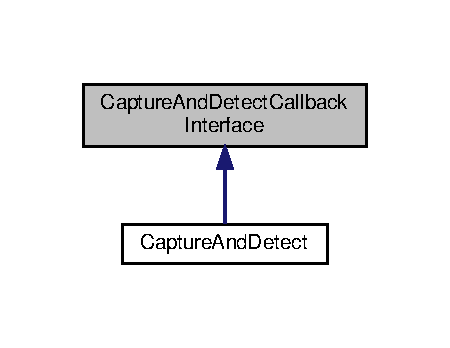
\includegraphics[width=216pt]{classCaptureAndDetectCallbackInterface__inherit__graph}
\end{center}
\end{figure}
\subsection*{Public Member Functions}
\begin{DoxyCompactItemize}
\item 
virtual void \hyperlink{classCaptureAndDetectCallbackInterface_ae833754fc1c2bb1450e958ef619e9153}{new\+Frame} (Mat)=0
\begin{DoxyCompactList}\small\item\em virtual method to update new\+Frame \end{DoxyCompactList}\item 
virtual bool \hyperlink{classCaptureAndDetectCallbackInterface_a64755838dd5592bae3ca06b4c5a0d72f}{check\+For\+Palm} ()=0
\begin{DoxyCompactList}\small\item\em virtual method to check if fist in image \end{DoxyCompactList}\item 
virtual void \hyperlink{classCaptureAndDetectCallbackInterface_a259dc71fd5d02424b91906d708e7de1f}{add\+To\+Buffer} (\hyperlink{classFingerAndCoordinates}{Finger\+And\+Coordinates})=0
\begin{DoxyCompactList}\small\item\em virtual method to add data to buffer \end{DoxyCompactList}\end{DoxyCompactItemize}


\subsection{Detailed Description}
Callback interface for \hyperlink{classCaptureAndDetect}{Capture\+And\+Detect}. 

\subsection{Member Function Documentation}
\mbox{\Hypertarget{classCaptureAndDetectCallbackInterface_a259dc71fd5d02424b91906d708e7de1f}\label{classCaptureAndDetectCallbackInterface_a259dc71fd5d02424b91906d708e7de1f}} 
\index{Capture\+And\+Detect\+Callback\+Interface@{Capture\+And\+Detect\+Callback\+Interface}!add\+To\+Buffer@{add\+To\+Buffer}}
\index{add\+To\+Buffer@{add\+To\+Buffer}!Capture\+And\+Detect\+Callback\+Interface@{Capture\+And\+Detect\+Callback\+Interface}}
\subsubsection{\texorpdfstring{add\+To\+Buffer()}{addToBuffer()}}
{\footnotesize\ttfamily virtual void Capture\+And\+Detect\+Callback\+Interface\+::add\+To\+Buffer (\begin{DoxyParamCaption}\item[{\hyperlink{classFingerAndCoordinates}{Finger\+And\+Coordinates}}]{ }\end{DoxyParamCaption})\hspace{0.3cm}{\ttfamily [pure virtual]}}



virtual method to add data to buffer 



Implemented in \hyperlink{classCaptureAndDetect_af376ab5418f7b235ee181d574da71fd6}{Capture\+And\+Detect}.

\mbox{\Hypertarget{classCaptureAndDetectCallbackInterface_a64755838dd5592bae3ca06b4c5a0d72f}\label{classCaptureAndDetectCallbackInterface_a64755838dd5592bae3ca06b4c5a0d72f}} 
\index{Capture\+And\+Detect\+Callback\+Interface@{Capture\+And\+Detect\+Callback\+Interface}!check\+For\+Palm@{check\+For\+Palm}}
\index{check\+For\+Palm@{check\+For\+Palm}!Capture\+And\+Detect\+Callback\+Interface@{Capture\+And\+Detect\+Callback\+Interface}}
\subsubsection{\texorpdfstring{check\+For\+Palm()}{checkForPalm()}}
{\footnotesize\ttfamily virtual bool Capture\+And\+Detect\+Callback\+Interface\+::check\+For\+Palm (\begin{DoxyParamCaption}{ }\end{DoxyParamCaption})\hspace{0.3cm}{\ttfamily [pure virtual]}}



virtual method to check if fist in image 



Implemented in \hyperlink{classCaptureAndDetect_a1620075ba1bf4d52a4e455c20f7ac3d1}{Capture\+And\+Detect}.

\mbox{\Hypertarget{classCaptureAndDetectCallbackInterface_ae833754fc1c2bb1450e958ef619e9153}\label{classCaptureAndDetectCallbackInterface_ae833754fc1c2bb1450e958ef619e9153}} 
\index{Capture\+And\+Detect\+Callback\+Interface@{Capture\+And\+Detect\+Callback\+Interface}!new\+Frame@{new\+Frame}}
\index{new\+Frame@{new\+Frame}!Capture\+And\+Detect\+Callback\+Interface@{Capture\+And\+Detect\+Callback\+Interface}}
\subsubsection{\texorpdfstring{new\+Frame()}{newFrame()}}
{\footnotesize\ttfamily virtual void Capture\+And\+Detect\+Callback\+Interface\+::new\+Frame (\begin{DoxyParamCaption}\item[{Mat}]{ }\end{DoxyParamCaption})\hspace{0.3cm}{\ttfamily [pure virtual]}}



virtual method to update new\+Frame 



Implemented in \hyperlink{classCaptureAndDetect_a7f18d1c58b2ae4241766b36aa27385e9}{Capture\+And\+Detect}.



The documentation for this class was generated from the following file\+:\begin{DoxyCompactItemize}
\item 
src/gesture\+\_\+detection/\hyperlink{CaptureAndDetectCallbackInterface_8h}{Capture\+And\+Detect\+Callback\+Interface.\+h}\end{DoxyCompactItemize}

\hypertarget{classDisplayControl}{}\section{Display\+Control Class Reference}
\label{classDisplayControl}\index{Display\+Control@{Display\+Control}}


This is a class that is inheriting from the classes \hyperlink{classWindowAction}{Window\+Action}, \hyperlink{classKeyboardAction}{Keyboard\+Action}, \hyperlink{classMouseAction}{Mouse\+Action}, \hyperlink{classVolumeControl}{Volume\+Control}, and \hyperlink{classDisplayControlCallbackInterface}{Display\+Control\+Callback\+Interface}.  




{\ttfamily \#include $<$Display\+Control.\+h$>$}



Inheritance diagram for Display\+Control\+:\nopagebreak
\begin{figure}[H]
\begin{center}
\leavevmode
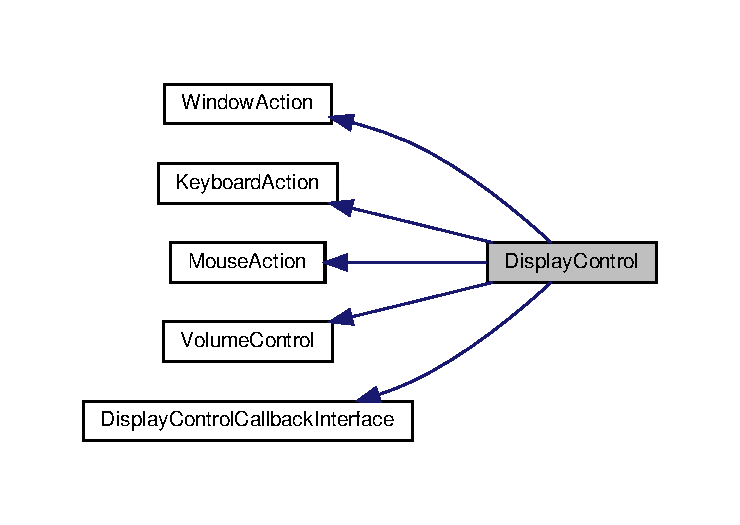
\includegraphics[width=350pt]{classDisplayControl__inherit__graph}
\end{center}
\end{figure}


Collaboration diagram for Display\+Control\+:\nopagebreak
\begin{figure}[H]
\begin{center}
\leavevmode
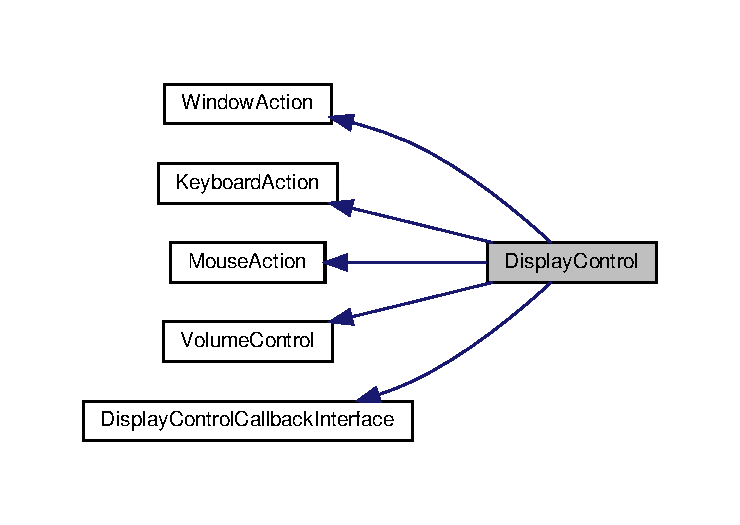
\includegraphics[width=350pt]{classDisplayControl__coll__graph}
\end{center}
\end{figure}
\subsection*{Public Member Functions}
\begin{DoxyCompactItemize}
\item 
\hyperlink{classDisplayControl_a4d2a5053b250bbd1f3103795cb29fcde}{Display\+Control} (Display $\ast$d)
\item 
void \hyperlink{classDisplayControl_aa8c509a1e17ba12d164dcfe43cf281d4}{do\+Mouse\+Move} (int, int) override
\item 
void \hyperlink{classDisplayControl_aa5af48425f7ba40012b2a7db5fabed45}{do\+Key\+Press} (int) override
\item 
void \hyperlink{classDisplayControl_a8a361b4c25ef55b86b5c2d178ffa516f}{do\+Increase\+Volume} () override
\item 
void \hyperlink{classDisplayControl_a874fa3f6b3e4cf465db62a4eba1c1dd1}{do\+Reduce\+Volume} () override
\item 
void \hyperlink{classDisplayControl_a210411b559d8c3ffb1498f49cfa26a6d}{do\+Unmute} () override
\item 
void \hyperlink{classDisplayControl_a25f685ea6bf001e53c7d17410f2a24ea}{do\+Mute\+Unmute} () override
\item 
void \hyperlink{classDisplayControl_a5f45c36e699afa1d56b2af78e5125aca}{do\+Button\+Press} (int) override
\item 
void \hyperlink{classDisplayControl_aca4208c53cac28e164e7949effdc04cd}{do\+Window\+Move} (int, int) override
\item 
void \hyperlink{classDisplayControl_ad5fa763a77c680ce7b2089c6d79c4eb7}{do\+Window\+Minimize} () override
\end{DoxyCompactItemize}


\subsection{Detailed Description}
This is a class that is inheriting from the classes \hyperlink{classWindowAction}{Window\+Action}, \hyperlink{classKeyboardAction}{Keyboard\+Action}, \hyperlink{classMouseAction}{Mouse\+Action}, \hyperlink{classVolumeControl}{Volume\+Control}, and \hyperlink{classDisplayControlCallbackInterface}{Display\+Control\+Callback\+Interface}. 

This class is used in order to concisely encapsulate the classes for keyboard,window, mouse and volume control into a single class so that they can be used in a callback function without the user needing to create objects for each of those classes any of the methods from the parent classes can be called by simply using dot notation 

\subsection{Constructor \& Destructor Documentation}
\mbox{\Hypertarget{classDisplayControl_a4d2a5053b250bbd1f3103795cb29fcde}\label{classDisplayControl_a4d2a5053b250bbd1f3103795cb29fcde}} 
\index{Display\+Control@{Display\+Control}!Display\+Control@{Display\+Control}}
\index{Display\+Control@{Display\+Control}!Display\+Control@{Display\+Control}}
\subsubsection{\texorpdfstring{Display\+Control()}{DisplayControl()}}
{\footnotesize\ttfamily Display\+Control\+::\+Display\+Control (\begin{DoxyParamCaption}\item[{Display $\ast$}]{d }\end{DoxyParamCaption})}

Constructor that takes in a display variable


\begin{DoxyParams}{Parameters}
{\em d} & The display to use. \\
\hline
\end{DoxyParams}


\subsection{Member Function Documentation}
\mbox{\Hypertarget{classDisplayControl_a5f45c36e699afa1d56b2af78e5125aca}\label{classDisplayControl_a5f45c36e699afa1d56b2af78e5125aca}} 
\index{Display\+Control@{Display\+Control}!do\+Button\+Press@{do\+Button\+Press}}
\index{do\+Button\+Press@{do\+Button\+Press}!Display\+Control@{Display\+Control}}
\subsubsection{\texorpdfstring{do\+Button\+Press()}{doButtonPress()}}
{\footnotesize\ttfamily void Display\+Control\+::do\+Button\+Press (\begin{DoxyParamCaption}\item[{int}]{x }\end{DoxyParamCaption})\hspace{0.3cm}{\ttfamily [override]}, {\ttfamily [virtual]}}

overrides the Display\+Control\+Interface method and uses \hyperlink{classMouseAction}{Mouse\+Action} to press\+Button 

Implements \hyperlink{classDisplayControlCallbackInterface_a55f329e2ab41d237f03b166349d2467e}{Display\+Control\+Callback\+Interface}.

\mbox{\Hypertarget{classDisplayControl_a8a361b4c25ef55b86b5c2d178ffa516f}\label{classDisplayControl_a8a361b4c25ef55b86b5c2d178ffa516f}} 
\index{Display\+Control@{Display\+Control}!do\+Increase\+Volume@{do\+Increase\+Volume}}
\index{do\+Increase\+Volume@{do\+Increase\+Volume}!Display\+Control@{Display\+Control}}
\subsubsection{\texorpdfstring{do\+Increase\+Volume()}{doIncreaseVolume()}}
{\footnotesize\ttfamily void Display\+Control\+::do\+Increase\+Volume (\begin{DoxyParamCaption}{ }\end{DoxyParamCaption})\hspace{0.3cm}{\ttfamily [override]}, {\ttfamily [virtual]}}

overrides the Display\+Control\+Interface method and uses \hyperlink{classVolumeControl}{Volume\+Control} to increase\+Volume 

Implements \hyperlink{classDisplayControlCallbackInterface_a78d7afe70cf3d2f524824efe087f0069}{Display\+Control\+Callback\+Interface}.

\mbox{\Hypertarget{classDisplayControl_aa5af48425f7ba40012b2a7db5fabed45}\label{classDisplayControl_aa5af48425f7ba40012b2a7db5fabed45}} 
\index{Display\+Control@{Display\+Control}!do\+Key\+Press@{do\+Key\+Press}}
\index{do\+Key\+Press@{do\+Key\+Press}!Display\+Control@{Display\+Control}}
\subsubsection{\texorpdfstring{do\+Key\+Press()}{doKeyPress()}}
{\footnotesize\ttfamily void Display\+Control\+::do\+Key\+Press (\begin{DoxyParamCaption}\item[{int}]{x }\end{DoxyParamCaption})\hspace{0.3cm}{\ttfamily [override]}, {\ttfamily [virtual]}}

overrides the Display\+Control\+Interface method and uses \hyperlink{classKeyboardAction}{Keyboard\+Action} to press\+Key 

Implements \hyperlink{classDisplayControlCallbackInterface_afdf32e210ff484bfd669b9de84c94dba}{Display\+Control\+Callback\+Interface}.

\mbox{\Hypertarget{classDisplayControl_aa8c509a1e17ba12d164dcfe43cf281d4}\label{classDisplayControl_aa8c509a1e17ba12d164dcfe43cf281d4}} 
\index{Display\+Control@{Display\+Control}!do\+Mouse\+Move@{do\+Mouse\+Move}}
\index{do\+Mouse\+Move@{do\+Mouse\+Move}!Display\+Control@{Display\+Control}}
\subsubsection{\texorpdfstring{do\+Mouse\+Move()}{doMouseMove()}}
{\footnotesize\ttfamily void Display\+Control\+::do\+Mouse\+Move (\begin{DoxyParamCaption}\item[{int}]{x,  }\item[{int}]{y }\end{DoxyParamCaption})\hspace{0.3cm}{\ttfamily [override]}, {\ttfamily [virtual]}}

overrides the Display\+Control\+Interface method and uses \hyperlink{classMouseAction}{Mouse\+Action} to move\+Mouse 

Implements \hyperlink{classDisplayControlCallbackInterface_ab7abee0745e5313dc50fe33c0206310a}{Display\+Control\+Callback\+Interface}.

\mbox{\Hypertarget{classDisplayControl_a25f685ea6bf001e53c7d17410f2a24ea}\label{classDisplayControl_a25f685ea6bf001e53c7d17410f2a24ea}} 
\index{Display\+Control@{Display\+Control}!do\+Mute\+Unmute@{do\+Mute\+Unmute}}
\index{do\+Mute\+Unmute@{do\+Mute\+Unmute}!Display\+Control@{Display\+Control}}
\subsubsection{\texorpdfstring{do\+Mute\+Unmute()}{doMuteUnmute()}}
{\footnotesize\ttfamily void Display\+Control\+::do\+Mute\+Unmute (\begin{DoxyParamCaption}{ }\end{DoxyParamCaption})\hspace{0.3cm}{\ttfamily [override]}, {\ttfamily [virtual]}}

overrides the Display\+Control\+Interface method and uses \hyperlink{classVolumeControl}{Volume\+Control} to mute\+Unmute\+Volume 

Implements \hyperlink{classDisplayControlCallbackInterface_a2826e548e2701baa4990422e0671b233}{Display\+Control\+Callback\+Interface}.

\mbox{\Hypertarget{classDisplayControl_a874fa3f6b3e4cf465db62a4eba1c1dd1}\label{classDisplayControl_a874fa3f6b3e4cf465db62a4eba1c1dd1}} 
\index{Display\+Control@{Display\+Control}!do\+Reduce\+Volume@{do\+Reduce\+Volume}}
\index{do\+Reduce\+Volume@{do\+Reduce\+Volume}!Display\+Control@{Display\+Control}}
\subsubsection{\texorpdfstring{do\+Reduce\+Volume()}{doReduceVolume()}}
{\footnotesize\ttfamily void Display\+Control\+::do\+Reduce\+Volume (\begin{DoxyParamCaption}{ }\end{DoxyParamCaption})\hspace{0.3cm}{\ttfamily [override]}, {\ttfamily [virtual]}}

overrides the Display\+Control\+Interface method and uses \hyperlink{classVolumeControl}{Volume\+Control} to reduce\+Volume 

Implements \hyperlink{classDisplayControlCallbackInterface_ac84cb33c6ffa7e818269e664d00fda6d}{Display\+Control\+Callback\+Interface}.

\mbox{\Hypertarget{classDisplayControl_a210411b559d8c3ffb1498f49cfa26a6d}\label{classDisplayControl_a210411b559d8c3ffb1498f49cfa26a6d}} 
\index{Display\+Control@{Display\+Control}!do\+Unmute@{do\+Unmute}}
\index{do\+Unmute@{do\+Unmute}!Display\+Control@{Display\+Control}}
\subsubsection{\texorpdfstring{do\+Unmute()}{doUnmute()}}
{\footnotesize\ttfamily void Display\+Control\+::do\+Unmute (\begin{DoxyParamCaption}{ }\end{DoxyParamCaption})\hspace{0.3cm}{\ttfamily [override]}, {\ttfamily [virtual]}}

overrides the Display\+Control\+Interface method and uses \hyperlink{classVolumeControl}{Volume\+Control} to unmute\+Volume 

Implements \hyperlink{classDisplayControlCallbackInterface_a24be31ca23631717ac789f2e98467015}{Display\+Control\+Callback\+Interface}.

\mbox{\Hypertarget{classDisplayControl_ad5fa763a77c680ce7b2089c6d79c4eb7}\label{classDisplayControl_ad5fa763a77c680ce7b2089c6d79c4eb7}} 
\index{Display\+Control@{Display\+Control}!do\+Window\+Minimize@{do\+Window\+Minimize}}
\index{do\+Window\+Minimize@{do\+Window\+Minimize}!Display\+Control@{Display\+Control}}
\subsubsection{\texorpdfstring{do\+Window\+Minimize()}{doWindowMinimize()}}
{\footnotesize\ttfamily void Display\+Control\+::do\+Window\+Minimize (\begin{DoxyParamCaption}{ }\end{DoxyParamCaption})\hspace{0.3cm}{\ttfamily [override]}, {\ttfamily [virtual]}}

overrides the Display\+Control\+Interface method and uses \hyperlink{classWindowAction}{Window\+Action} to minimize\+Window 

Implements \hyperlink{classDisplayControlCallbackInterface_a5457bccb953df7296b81b96db827896c}{Display\+Control\+Callback\+Interface}.

\mbox{\Hypertarget{classDisplayControl_aca4208c53cac28e164e7949effdc04cd}\label{classDisplayControl_aca4208c53cac28e164e7949effdc04cd}} 
\index{Display\+Control@{Display\+Control}!do\+Window\+Move@{do\+Window\+Move}}
\index{do\+Window\+Move@{do\+Window\+Move}!Display\+Control@{Display\+Control}}
\subsubsection{\texorpdfstring{do\+Window\+Move()}{doWindowMove()}}
{\footnotesize\ttfamily void Display\+Control\+::do\+Window\+Move (\begin{DoxyParamCaption}\item[{int}]{x,  }\item[{int}]{y }\end{DoxyParamCaption})\hspace{0.3cm}{\ttfamily [override]}, {\ttfamily [virtual]}}

overrides the Display\+Control\+Interface method and uses \hyperlink{classWindowAction}{Window\+Action} to move\+Window 

Implements \hyperlink{classDisplayControlCallbackInterface_af8f01d480c76ee88d2719a246b5d4135}{Display\+Control\+Callback\+Interface}.



The documentation for this class was generated from the following files\+:\begin{DoxyCompactItemize}
\item 
src/ubuntu\+\_\+controls/\hyperlink{DisplayControl_8h}{Display\+Control.\+h}\item 
src/ubuntu\+\_\+controls/\hyperlink{DisplayControl_8cpp}{Display\+Control.\+cpp}\end{DoxyCompactItemize}

\hypertarget{classDisplayControlCallbackInterface}{}\section{Display\+Control\+Callback\+Interface Class Reference}
\label{classDisplayControlCallbackInterface}\index{Display\+Control\+Callback\+Interface@{Display\+Control\+Callback\+Interface}}


{\ttfamily \#include $<$Display\+Control\+Callback\+Interface.\+h$>$}



Inheritance diagram for Display\+Control\+Callback\+Interface\+:\nopagebreak
\begin{figure}[H]
\begin{center}
\leavevmode
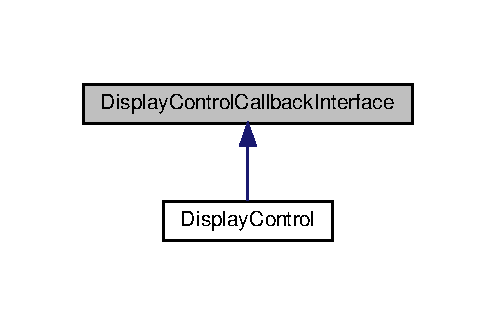
\includegraphics[width=238pt]{classDisplayControlCallbackInterface__inherit__graph}
\end{center}
\end{figure}
\subsection*{Public Member Functions}
\begin{DoxyCompactItemize}
\item 
virtual void \hyperlink{classDisplayControlCallbackInterface_ab7abee0745e5313dc50fe33c0206310a}{do\+Mouse\+Move} (int, int)=0
\item 
virtual void \hyperlink{classDisplayControlCallbackInterface_afdf32e210ff484bfd669b9de84c94dba}{do\+Key\+Press} (int)=0
\item 
virtual void \hyperlink{classDisplayControlCallbackInterface_a78d7afe70cf3d2f524824efe087f0069}{do\+Increase\+Volume} ()=0
\item 
virtual void \hyperlink{classDisplayControlCallbackInterface_ac84cb33c6ffa7e818269e664d00fda6d}{do\+Reduce\+Volume} ()=0
\item 
virtual void \hyperlink{classDisplayControlCallbackInterface_a2826e548e2701baa4990422e0671b233}{do\+Mute\+Unmute} ()=0
\item 
virtual void \hyperlink{classDisplayControlCallbackInterface_a24be31ca23631717ac789f2e98467015}{do\+Unmute} ()=0
\item 
virtual void \hyperlink{classDisplayControlCallbackInterface_a55f329e2ab41d237f03b166349d2467e}{do\+Button\+Press} (int)=0
\item 
virtual void \hyperlink{classDisplayControlCallbackInterface_af8f01d480c76ee88d2719a246b5d4135}{do\+Window\+Move} (int, int)=0
\item 
virtual void \hyperlink{classDisplayControlCallbackInterface_a5457bccb953df7296b81b96db827896c}{do\+Window\+Minimize} ()=0
\end{DoxyCompactItemize}


\subsection{Detailed Description}
An interface to use as callback. 

\subsection{Member Function Documentation}
\mbox{\Hypertarget{classDisplayControlCallbackInterface_a55f329e2ab41d237f03b166349d2467e}\label{classDisplayControlCallbackInterface_a55f329e2ab41d237f03b166349d2467e}} 
\index{Display\+Control\+Callback\+Interface@{Display\+Control\+Callback\+Interface}!do\+Button\+Press@{do\+Button\+Press}}
\index{do\+Button\+Press@{do\+Button\+Press}!Display\+Control\+Callback\+Interface@{Display\+Control\+Callback\+Interface}}
\subsubsection{\texorpdfstring{do\+Button\+Press()}{doButtonPress()}}
{\footnotesize\ttfamily virtual void Display\+Control\+Callback\+Interface\+::do\+Button\+Press (\begin{DoxyParamCaption}\item[{int}]{ }\end{DoxyParamCaption})\hspace{0.3cm}{\ttfamily [pure virtual]}}



Implemented in \hyperlink{classDisplayControl_a5f45c36e699afa1d56b2af78e5125aca}{Display\+Control}.

\mbox{\Hypertarget{classDisplayControlCallbackInterface_a78d7afe70cf3d2f524824efe087f0069}\label{classDisplayControlCallbackInterface_a78d7afe70cf3d2f524824efe087f0069}} 
\index{Display\+Control\+Callback\+Interface@{Display\+Control\+Callback\+Interface}!do\+Increase\+Volume@{do\+Increase\+Volume}}
\index{do\+Increase\+Volume@{do\+Increase\+Volume}!Display\+Control\+Callback\+Interface@{Display\+Control\+Callback\+Interface}}
\subsubsection{\texorpdfstring{do\+Increase\+Volume()}{doIncreaseVolume()}}
{\footnotesize\ttfamily virtual void Display\+Control\+Callback\+Interface\+::do\+Increase\+Volume (\begin{DoxyParamCaption}{ }\end{DoxyParamCaption})\hspace{0.3cm}{\ttfamily [pure virtual]}}



Implemented in \hyperlink{classDisplayControl_a8a361b4c25ef55b86b5c2d178ffa516f}{Display\+Control}.

\mbox{\Hypertarget{classDisplayControlCallbackInterface_afdf32e210ff484bfd669b9de84c94dba}\label{classDisplayControlCallbackInterface_afdf32e210ff484bfd669b9de84c94dba}} 
\index{Display\+Control\+Callback\+Interface@{Display\+Control\+Callback\+Interface}!do\+Key\+Press@{do\+Key\+Press}}
\index{do\+Key\+Press@{do\+Key\+Press}!Display\+Control\+Callback\+Interface@{Display\+Control\+Callback\+Interface}}
\subsubsection{\texorpdfstring{do\+Key\+Press()}{doKeyPress()}}
{\footnotesize\ttfamily virtual void Display\+Control\+Callback\+Interface\+::do\+Key\+Press (\begin{DoxyParamCaption}\item[{int}]{ }\end{DoxyParamCaption})\hspace{0.3cm}{\ttfamily [pure virtual]}}



Implemented in \hyperlink{classDisplayControl_aa5af48425f7ba40012b2a7db5fabed45}{Display\+Control}.

\mbox{\Hypertarget{classDisplayControlCallbackInterface_ab7abee0745e5313dc50fe33c0206310a}\label{classDisplayControlCallbackInterface_ab7abee0745e5313dc50fe33c0206310a}} 
\index{Display\+Control\+Callback\+Interface@{Display\+Control\+Callback\+Interface}!do\+Mouse\+Move@{do\+Mouse\+Move}}
\index{do\+Mouse\+Move@{do\+Mouse\+Move}!Display\+Control\+Callback\+Interface@{Display\+Control\+Callback\+Interface}}
\subsubsection{\texorpdfstring{do\+Mouse\+Move()}{doMouseMove()}}
{\footnotesize\ttfamily virtual void Display\+Control\+Callback\+Interface\+::do\+Mouse\+Move (\begin{DoxyParamCaption}\item[{int}]{,  }\item[{int}]{ }\end{DoxyParamCaption})\hspace{0.3cm}{\ttfamily [pure virtual]}}



Implemented in \hyperlink{classDisplayControl_aa8c509a1e17ba12d164dcfe43cf281d4}{Display\+Control}.

\mbox{\Hypertarget{classDisplayControlCallbackInterface_a2826e548e2701baa4990422e0671b233}\label{classDisplayControlCallbackInterface_a2826e548e2701baa4990422e0671b233}} 
\index{Display\+Control\+Callback\+Interface@{Display\+Control\+Callback\+Interface}!do\+Mute\+Unmute@{do\+Mute\+Unmute}}
\index{do\+Mute\+Unmute@{do\+Mute\+Unmute}!Display\+Control\+Callback\+Interface@{Display\+Control\+Callback\+Interface}}
\subsubsection{\texorpdfstring{do\+Mute\+Unmute()}{doMuteUnmute()}}
{\footnotesize\ttfamily virtual void Display\+Control\+Callback\+Interface\+::do\+Mute\+Unmute (\begin{DoxyParamCaption}{ }\end{DoxyParamCaption})\hspace{0.3cm}{\ttfamily [pure virtual]}}



Implemented in \hyperlink{classDisplayControl_a25f685ea6bf001e53c7d17410f2a24ea}{Display\+Control}.

\mbox{\Hypertarget{classDisplayControlCallbackInterface_ac84cb33c6ffa7e818269e664d00fda6d}\label{classDisplayControlCallbackInterface_ac84cb33c6ffa7e818269e664d00fda6d}} 
\index{Display\+Control\+Callback\+Interface@{Display\+Control\+Callback\+Interface}!do\+Reduce\+Volume@{do\+Reduce\+Volume}}
\index{do\+Reduce\+Volume@{do\+Reduce\+Volume}!Display\+Control\+Callback\+Interface@{Display\+Control\+Callback\+Interface}}
\subsubsection{\texorpdfstring{do\+Reduce\+Volume()}{doReduceVolume()}}
{\footnotesize\ttfamily virtual void Display\+Control\+Callback\+Interface\+::do\+Reduce\+Volume (\begin{DoxyParamCaption}{ }\end{DoxyParamCaption})\hspace{0.3cm}{\ttfamily [pure virtual]}}



Implemented in \hyperlink{classDisplayControl_a874fa3f6b3e4cf465db62a4eba1c1dd1}{Display\+Control}.

\mbox{\Hypertarget{classDisplayControlCallbackInterface_a24be31ca23631717ac789f2e98467015}\label{classDisplayControlCallbackInterface_a24be31ca23631717ac789f2e98467015}} 
\index{Display\+Control\+Callback\+Interface@{Display\+Control\+Callback\+Interface}!do\+Unmute@{do\+Unmute}}
\index{do\+Unmute@{do\+Unmute}!Display\+Control\+Callback\+Interface@{Display\+Control\+Callback\+Interface}}
\subsubsection{\texorpdfstring{do\+Unmute()}{doUnmute()}}
{\footnotesize\ttfamily virtual void Display\+Control\+Callback\+Interface\+::do\+Unmute (\begin{DoxyParamCaption}{ }\end{DoxyParamCaption})\hspace{0.3cm}{\ttfamily [pure virtual]}}



Implemented in \hyperlink{classDisplayControl_a210411b559d8c3ffb1498f49cfa26a6d}{Display\+Control}.

\mbox{\Hypertarget{classDisplayControlCallbackInterface_a5457bccb953df7296b81b96db827896c}\label{classDisplayControlCallbackInterface_a5457bccb953df7296b81b96db827896c}} 
\index{Display\+Control\+Callback\+Interface@{Display\+Control\+Callback\+Interface}!do\+Window\+Minimize@{do\+Window\+Minimize}}
\index{do\+Window\+Minimize@{do\+Window\+Minimize}!Display\+Control\+Callback\+Interface@{Display\+Control\+Callback\+Interface}}
\subsubsection{\texorpdfstring{do\+Window\+Minimize()}{doWindowMinimize()}}
{\footnotesize\ttfamily virtual void Display\+Control\+Callback\+Interface\+::do\+Window\+Minimize (\begin{DoxyParamCaption}{ }\end{DoxyParamCaption})\hspace{0.3cm}{\ttfamily [pure virtual]}}



Implemented in \hyperlink{classDisplayControl_ad5fa763a77c680ce7b2089c6d79c4eb7}{Display\+Control}.

\mbox{\Hypertarget{classDisplayControlCallbackInterface_af8f01d480c76ee88d2719a246b5d4135}\label{classDisplayControlCallbackInterface_af8f01d480c76ee88d2719a246b5d4135}} 
\index{Display\+Control\+Callback\+Interface@{Display\+Control\+Callback\+Interface}!do\+Window\+Move@{do\+Window\+Move}}
\index{do\+Window\+Move@{do\+Window\+Move}!Display\+Control\+Callback\+Interface@{Display\+Control\+Callback\+Interface}}
\subsubsection{\texorpdfstring{do\+Window\+Move()}{doWindowMove()}}
{\footnotesize\ttfamily virtual void Display\+Control\+Callback\+Interface\+::do\+Window\+Move (\begin{DoxyParamCaption}\item[{int}]{,  }\item[{int}]{ }\end{DoxyParamCaption})\hspace{0.3cm}{\ttfamily [pure virtual]}}



Implemented in \hyperlink{classDisplayControl_aca4208c53cac28e164e7949effdc04cd}{Display\+Control}.



The documentation for this class was generated from the following file\+:\begin{DoxyCompactItemize}
\item 
src/ubuntu\+\_\+controls/\hyperlink{DisplayControlCallbackInterface_8h}{Display\+Control\+Callback\+Interface.\+h}\end{DoxyCompactItemize}

\hypertarget{classFingerAndCoordinates}{}\section{Finger\+And\+Coordinates Class Reference}
\label{classFingerAndCoordinates}\index{Finger\+And\+Coordinates@{Finger\+And\+Coordinates}}


class to store the information detected by the \hyperlink{classFingerCounter}{Finger\+Counter}.  




{\ttfamily \#include $<$Finger\+And\+Coordinates.\+h$>$}

\subsection*{Public Member Functions}
\begin{DoxyCompactItemize}
\item 
\hyperlink{classFingerAndCoordinates_a9d24b8b3b3237f0a39762a52daf6f6a5}{Finger\+And\+Coordinates} ()
\item 
\hyperlink{classFingerAndCoordinates_a907ced00a2a2075194c38b9a356bfb60}{Finger\+And\+Coordinates} (\hyperlink{Commands_8h_a1939e90743463fb34c8c571ec0590430}{Commands}, int \hyperlink{classFingerAndCoordinates_ac68efb78d744788be7e3105627fe9320}{x}=0, int \hyperlink{classFingerAndCoordinates_a7a5165f9b4a0304ceb8bdcd5f35c2c77}{y}=0)
\end{DoxyCompactItemize}
\subsection*{Public Attributes}
\begin{DoxyCompactItemize}
\item 
int \hyperlink{classFingerAndCoordinates_af94d8ca7cd08d7144ec919fa997120c0}{command} = 0
\begin{DoxyCompactList}\small\item\em stores the command E\+N\+UM \end{DoxyCompactList}\item 
int \hyperlink{classFingerAndCoordinates_ac68efb78d744788be7e3105627fe9320}{x}
\begin{DoxyCompactList}\small\item\em int to store the x coordinate of the highest point \end{DoxyCompactList}\item 
int \hyperlink{classFingerAndCoordinates_a7a5165f9b4a0304ceb8bdcd5f35c2c77}{y}
\begin{DoxyCompactList}\small\item\em int to store the y coordinate of the highest point \end{DoxyCompactList}\end{DoxyCompactItemize}


\subsection{Detailed Description}
class to store the information detected by the \hyperlink{classFingerCounter}{Finger\+Counter}. 

\subsection{Constructor \& Destructor Documentation}
\mbox{\Hypertarget{classFingerAndCoordinates_a9d24b8b3b3237f0a39762a52daf6f6a5}\label{classFingerAndCoordinates_a9d24b8b3b3237f0a39762a52daf6f6a5}} 
\index{Finger\+And\+Coordinates@{Finger\+And\+Coordinates}!Finger\+And\+Coordinates@{Finger\+And\+Coordinates}}
\index{Finger\+And\+Coordinates@{Finger\+And\+Coordinates}!Finger\+And\+Coordinates@{Finger\+And\+Coordinates}}
\subsubsection{\texorpdfstring{Finger\+And\+Coordinates()}{FingerAndCoordinates()}\hspace{0.1cm}{\footnotesize\ttfamily [1/2]}}
{\footnotesize\ttfamily Finger\+And\+Coordinates\+::\+Finger\+And\+Coordinates (\begin{DoxyParamCaption}{ }\end{DoxyParamCaption})}

Default constructor \mbox{\Hypertarget{classFingerAndCoordinates_a907ced00a2a2075194c38b9a356bfb60}\label{classFingerAndCoordinates_a907ced00a2a2075194c38b9a356bfb60}} 
\index{Finger\+And\+Coordinates@{Finger\+And\+Coordinates}!Finger\+And\+Coordinates@{Finger\+And\+Coordinates}}
\index{Finger\+And\+Coordinates@{Finger\+And\+Coordinates}!Finger\+And\+Coordinates@{Finger\+And\+Coordinates}}
\subsubsection{\texorpdfstring{Finger\+And\+Coordinates()}{FingerAndCoordinates()}\hspace{0.1cm}{\footnotesize\ttfamily [2/2]}}
{\footnotesize\ttfamily Finger\+And\+Coordinates\+::\+Finger\+And\+Coordinates (\begin{DoxyParamCaption}\item[{\hyperlink{Commands_8h_a1939e90743463fb34c8c571ec0590430}{Commands}}]{new\+Command,  }\item[{int}]{x = {\ttfamily 0},  }\item[{int}]{y = {\ttfamily 0} }\end{DoxyParamCaption})}

This function is a constructor for the \hyperlink{classFingerAndCoordinates}{Finger\+And\+Coordinates} class.


\begin{DoxyParams}{Parameters}
{\em new\+Command} & The command that was detected. \\
\hline
{\em x} & The x coordinate of the highest point \\
\hline
{\em y} & The y coordinate of the highest point. \\
\hline
\end{DoxyParams}


\subsection{Member Data Documentation}
\mbox{\Hypertarget{classFingerAndCoordinates_af94d8ca7cd08d7144ec919fa997120c0}\label{classFingerAndCoordinates_af94d8ca7cd08d7144ec919fa997120c0}} 
\index{Finger\+And\+Coordinates@{Finger\+And\+Coordinates}!command@{command}}
\index{command@{command}!Finger\+And\+Coordinates@{Finger\+And\+Coordinates}}
\subsubsection{\texorpdfstring{command}{command}}
{\footnotesize\ttfamily int Finger\+And\+Coordinates\+::command = 0}



stores the command E\+N\+UM 

\mbox{\Hypertarget{classFingerAndCoordinates_ac68efb78d744788be7e3105627fe9320}\label{classFingerAndCoordinates_ac68efb78d744788be7e3105627fe9320}} 
\index{Finger\+And\+Coordinates@{Finger\+And\+Coordinates}!x@{x}}
\index{x@{x}!Finger\+And\+Coordinates@{Finger\+And\+Coordinates}}
\subsubsection{\texorpdfstring{x}{x}}
{\footnotesize\ttfamily int Finger\+And\+Coordinates\+::x}



int to store the x coordinate of the highest point 

\mbox{\Hypertarget{classFingerAndCoordinates_a7a5165f9b4a0304ceb8bdcd5f35c2c77}\label{classFingerAndCoordinates_a7a5165f9b4a0304ceb8bdcd5f35c2c77}} 
\index{Finger\+And\+Coordinates@{Finger\+And\+Coordinates}!y@{y}}
\index{y@{y}!Finger\+And\+Coordinates@{Finger\+And\+Coordinates}}
\subsubsection{\texorpdfstring{y}{y}}
{\footnotesize\ttfamily int Finger\+And\+Coordinates\+::y}



int to store the y coordinate of the highest point 



The documentation for this class was generated from the following files\+:\begin{DoxyCompactItemize}
\item 
src/gesture\+\_\+detection/\hyperlink{FingerAndCoordinates_8h}{Finger\+And\+Coordinates.\+h}\item 
src/gesture\+\_\+detection/\hyperlink{FingerAndCoordinates_8cpp}{Finger\+And\+Coordinates.\+cpp}\end{DoxyCompactItemize}

\hypertarget{classFingerCounter}{}\section{Finger\+Counter Class Reference}
\label{classFingerCounter}\index{Finger\+Counter@{Finger\+Counter}}


checks the number of fingers and sends the respective command to be processed.  




{\ttfamily \#include $<$Finger\+Counter.\+h$>$}

\subsection*{Public Member Functions}
\begin{DoxyCompactItemize}
\item 
\hyperlink{classFingerCounter_a2f6f5bc97506e87dc7acc6e02579a916}{Finger\+Counter} (void)
\item 
\hyperlink{classFingerAndCoordinates}{Finger\+And\+Coordinates} \hyperlink{classFingerCounter_a611201352a86dd943f866c1be9507081}{find\+Fingers\+Count} (Mat input\+\_\+image, Mat frame)
\item 
void \hyperlink{classFingerCounter_a5b5aabaa39ff05c70a873b4c2a7869f9}{Connect\+Callback} (\hyperlink{classCaptureAndDetectCallbackInterface}{Capture\+And\+Detect\+Callback\+Interface} $\ast$)
\end{DoxyCompactItemize}


\subsection{Detailed Description}
checks the number of fingers and sends the respective command to be processed. 

This class is called from the \hyperlink{classCaptureAndDetect}{Capture\+And\+Detect} after the initial image processing is done, the fingers and stored in the buffer. Once the buffer size is 15 the finger that occurs the most number of times in the buffer is considered and the appropriate command is sent. If finger is one or 3 then the coordinates are sent until a new finger is detected. 

\subsection{Constructor \& Destructor Documentation}
\mbox{\Hypertarget{classFingerCounter_a2f6f5bc97506e87dc7acc6e02579a916}\label{classFingerCounter_a2f6f5bc97506e87dc7acc6e02579a916}} 
\index{Finger\+Counter@{Finger\+Counter}!Finger\+Counter@{Finger\+Counter}}
\index{Finger\+Counter@{Finger\+Counter}!Finger\+Counter@{Finger\+Counter}}
\subsubsection{\texorpdfstring{Finger\+Counter()}{FingerCounter()}}
{\footnotesize\ttfamily Finger\+Counter\+::\+Finger\+Counter (\begin{DoxyParamCaption}\item[{void}]{ }\end{DoxyParamCaption})}

The constructor for the \hyperlink{classFingerCounter}{Finger\+Counter} class. Initializes the colors and iir filters. 

\subsection{Member Function Documentation}
\mbox{\Hypertarget{classFingerCounter_a5b5aabaa39ff05c70a873b4c2a7869f9}\label{classFingerCounter_a5b5aabaa39ff05c70a873b4c2a7869f9}} 
\index{Finger\+Counter@{Finger\+Counter}!Connect\+Callback@{Connect\+Callback}}
\index{Connect\+Callback@{Connect\+Callback}!Finger\+Counter@{Finger\+Counter}}
\subsubsection{\texorpdfstring{Connect\+Callback()}{ConnectCallback()}}
{\footnotesize\ttfamily void Finger\+Counter\+::\+Connect\+Callback (\begin{DoxyParamCaption}\item[{\hyperlink{classCaptureAndDetectCallbackInterface}{Capture\+And\+Detect\+Callback\+Interface} $\ast$}]{callback }\end{DoxyParamCaption})}

This function is used to connect the callback interface of \hyperlink{classCaptureAndDetect}{Capture\+And\+Detect} with this class


\begin{DoxyParams}{Parameters}
{\em callback} & The callback function that will be called when the fist is detected. \\
\hline
\end{DoxyParams}
\mbox{\Hypertarget{classFingerCounter_a611201352a86dd943f866c1be9507081}\label{classFingerCounter_a611201352a86dd943f866c1be9507081}} 
\index{Finger\+Counter@{Finger\+Counter}!find\+Fingers\+Count@{find\+Fingers\+Count}}
\index{find\+Fingers\+Count@{find\+Fingers\+Count}!Finger\+Counter@{Finger\+Counter}}
\subsubsection{\texorpdfstring{find\+Fingers\+Count()}{findFingersCount()}}
{\footnotesize\ttfamily \hyperlink{classFingerAndCoordinates}{Finger\+And\+Coordinates} Finger\+Counter\+::find\+Fingers\+Count (\begin{DoxyParamCaption}\item[{Mat}]{input\+\_\+image,  }\item[{Mat}]{frame }\end{DoxyParamCaption})}

It finds the contours of the hand, finds the convex hull and the defects, and then counts the number of fingers


\begin{DoxyParams}{Parameters}
{\em input\+\_\+image} & The image that we want to find the fingers in. \\
\hline
{\em frame} & The frame from the camera\\
\hline
\end{DoxyParams}
\begin{DoxyReturn}{Returns}
a struct of type \hyperlink{classFingerAndCoordinates}{Finger\+And\+Coordinates}. 
\end{DoxyReturn}


The documentation for this class was generated from the following files\+:\begin{DoxyCompactItemize}
\item 
src/gesture\+\_\+detection/\hyperlink{FingerCounter_8h}{Finger\+Counter.\+h}\item 
src/gesture\+\_\+detection/\hyperlink{FingerCounter_8cpp}{Finger\+Counter.\+cpp}\end{DoxyCompactItemize}

\hypertarget{classKeyboardAction}{}\section{Keyboard\+Action Class Reference}
\label{classKeyboardAction}\index{Keyboard\+Action@{Keyboard\+Action}}


A wrapper class for Keyboard Event.  




{\ttfamily \#include $<$Keyboard\+Action.\+h$>$}



Inheritance diagram for Keyboard\+Action\+:\nopagebreak
\begin{figure}[H]
\begin{center}
\leavevmode
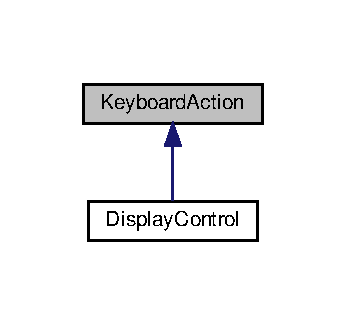
\includegraphics[width=166pt]{classKeyboardAction__inherit__graph}
\end{center}
\end{figure}
\subsection*{Public Member Functions}
\begin{DoxyCompactItemize}
\item 
\hyperlink{classKeyboardAction_af59163694e9b55ceaa75d779363e7fc9}{Keyboard\+Action} (Display $\ast$d)
\item 
void \hyperlink{classKeyboardAction_ab09e3956685d6fb11cd1cdf86a673b48}{press\+Key} (int k)
\end{DoxyCompactItemize}


\subsection{Detailed Description}
A wrapper class for Keyboard Event. 

\subsection{Constructor \& Destructor Documentation}
\mbox{\Hypertarget{classKeyboardAction_af59163694e9b55ceaa75d779363e7fc9}\label{classKeyboardAction_af59163694e9b55ceaa75d779363e7fc9}} 
\index{Keyboard\+Action@{Keyboard\+Action}!Keyboard\+Action@{Keyboard\+Action}}
\index{Keyboard\+Action@{Keyboard\+Action}!Keyboard\+Action@{Keyboard\+Action}}
\subsubsection{\texorpdfstring{Keyboard\+Action()}{KeyboardAction()}}
{\footnotesize\ttfamily Keyboard\+Action\+::\+Keyboard\+Action (\begin{DoxyParamCaption}\item[{Display $\ast$}]{d }\end{DoxyParamCaption})}

Constructor It takes a Display object as an argument and assigns it to the display variable.


\begin{DoxyParams}{Parameters}
{\em d} & The display to use. \\
\hline
\end{DoxyParams}


\subsection{Member Function Documentation}
\mbox{\Hypertarget{classKeyboardAction_ab09e3956685d6fb11cd1cdf86a673b48}\label{classKeyboardAction_ab09e3956685d6fb11cd1cdf86a673b48}} 
\index{Keyboard\+Action@{Keyboard\+Action}!press\+Key@{press\+Key}}
\index{press\+Key@{press\+Key}!Keyboard\+Action@{Keyboard\+Action}}
\subsubsection{\texorpdfstring{press\+Key()}{pressKey()}}
{\footnotesize\ttfamily void Keyboard\+Action\+::press\+Key (\begin{DoxyParamCaption}\item[{int}]{k }\end{DoxyParamCaption})}

Wrapper function for pressing Button


\begin{DoxyParams}{Parameters}
{\em k} & the keycode of the button to press. \\
\hline
\end{DoxyParams}


The documentation for this class was generated from the following files\+:\begin{DoxyCompactItemize}
\item 
src/ubuntu\+\_\+controls/\hyperlink{KeyboardAction_8h}{Keyboard\+Action.\+h}\item 
src/ubuntu\+\_\+controls/\hyperlink{KeyboardAction_8cpp}{Keyboard\+Action.\+cpp}\end{DoxyCompactItemize}

\hypertarget{classKeyboardEvent}{}\section{Keyboard\+Event Class Reference}
\label{classKeyboardEvent}\index{Keyboard\+Event@{Keyboard\+Event}}


Used to send keyboard events.  




{\ttfamily \#include $<$Keyboard\+Event.\+h$>$}

\subsection*{Public Member Functions}
\begin{DoxyCompactItemize}
\item 
\hyperlink{classKeyboardEvent_a5a4efca276ce847a471b228c4a114bc7}{Keyboard\+Event} (void)
\item 
X\+Key\+Event \hyperlink{classKeyboardEvent_a84e25f7a086a015007fe877a55d9444e}{create\+Key\+Event} (Display $\ast$display, Window \&win, Window \&win\+Root, bool press, int keycode, int modifiers)
\item 
void \hyperlink{classKeyboardEvent_aea537f2a22fc1f162fd81b5d039eb053}{key\+Press} (Display $\ast$display, int keycode)
\end{DoxyCompactItemize}


\subsection{Detailed Description}
Used to send keyboard events. 

\subsection{Constructor \& Destructor Documentation}
\mbox{\Hypertarget{classKeyboardEvent_a5a4efca276ce847a471b228c4a114bc7}\label{classKeyboardEvent_a5a4efca276ce847a471b228c4a114bc7}} 
\index{Keyboard\+Event@{Keyboard\+Event}!Keyboard\+Event@{Keyboard\+Event}}
\index{Keyboard\+Event@{Keyboard\+Event}!Keyboard\+Event@{Keyboard\+Event}}
\subsubsection{\texorpdfstring{Keyboard\+Event()}{KeyboardEvent()}}
{\footnotesize\ttfamily Keyboard\+Event\+::\+Keyboard\+Event (\begin{DoxyParamCaption}\item[{void}]{ }\end{DoxyParamCaption})}



\subsection{Member Function Documentation}
\mbox{\Hypertarget{classKeyboardEvent_a84e25f7a086a015007fe877a55d9444e}\label{classKeyboardEvent_a84e25f7a086a015007fe877a55d9444e}} 
\index{Keyboard\+Event@{Keyboard\+Event}!create\+Key\+Event@{create\+Key\+Event}}
\index{create\+Key\+Event@{create\+Key\+Event}!Keyboard\+Event@{Keyboard\+Event}}
\subsubsection{\texorpdfstring{create\+Key\+Event()}{createKeyEvent()}}
{\footnotesize\ttfamily X\+Key\+Event Keyboard\+Event\+::create\+Key\+Event (\begin{DoxyParamCaption}\item[{Display $\ast$}]{display,  }\item[{Window \&}]{win,  }\item[{Window \&}]{win\+Root,  }\item[{bool}]{press,  }\item[{int}]{keycode,  }\item[{int}]{modifiers }\end{DoxyParamCaption})}

It creates a key event that can be sent to the X server


\begin{DoxyParams}{Parameters}
{\em display} & The display that the event is occuring on. \\
\hline
{\em win} & The window that the event is occuring on. \\
\hline
{\em win\+Root} & The root window is the first window that all windows in the display are descended from. \\
\hline
{\em press} & whether the key is pressed or released \\
\hline
{\em keycode} & The X11 defined code for the key that is simulated. \\
\hline
{\em modifiers} & This is a bitmask that specifies the modifier keys that are pressed.\\
\hline
\end{DoxyParams}
\begin{DoxyReturn}{Returns}
A X\+Key\+Event object 
\end{DoxyReturn}
\mbox{\Hypertarget{classKeyboardEvent_aea537f2a22fc1f162fd81b5d039eb053}\label{classKeyboardEvent_aea537f2a22fc1f162fd81b5d039eb053}} 
\index{Keyboard\+Event@{Keyboard\+Event}!key\+Press@{key\+Press}}
\index{key\+Press@{key\+Press}!Keyboard\+Event@{Keyboard\+Event}}
\subsubsection{\texorpdfstring{key\+Press()}{keyPress()}}
{\footnotesize\ttfamily void Keyboard\+Event\+::key\+Press (\begin{DoxyParamCaption}\item[{Display $\ast$}]{display,  }\item[{int}]{keycode }\end{DoxyParamCaption})}

It creates a fake key press event and sends it to the window which currently has the keyboard focus


\begin{DoxyParams}{Parameters}
{\em display} & The Display to send the event to. \\
\hline
{\em keycode} & The keycode of the key to be pressed. \\
\hline
\end{DoxyParams}


The documentation for this class was generated from the following files\+:\begin{DoxyCompactItemize}
\item 
src/ubuntu\+\_\+controls/\hyperlink{KeyboardEvent_8h}{Keyboard\+Event.\+h}\item 
src/ubuntu\+\_\+controls/\hyperlink{KeyboardEvent_8cpp}{Keyboard\+Event.\+cpp}\end{DoxyCompactItemize}

\hypertarget{classMouseAction}{}\section{Mouse\+Action Class Reference}
\label{classMouseAction}\index{Mouse\+Action@{Mouse\+Action}}


A wrapper class for mouse control.  




{\ttfamily \#include $<$Mouse\+Action.\+h$>$}



Inheritance diagram for Mouse\+Action\+:\nopagebreak
\begin{figure}[H]
\begin{center}
\leavevmode
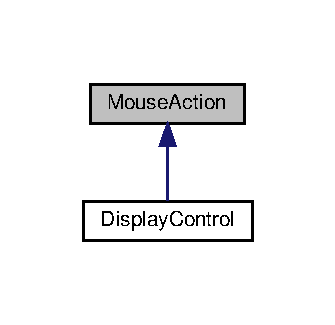
\includegraphics[width=161pt]{classMouseAction__inherit__graph}
\end{center}
\end{figure}
\subsection*{Public Member Functions}
\begin{DoxyCompactItemize}
\item 
\hyperlink{classMouseAction_a42e540b994144f3f8775baded5370b14}{Mouse\+Action} (Display $\ast$d, X\+Event e)
\item 
void \hyperlink{classMouseAction_aa017b86a7e358e7a74a8ec50a5a191cf}{press\+Button} (int button)
\item 
void \hyperlink{classMouseAction_ab1ac193e88baf8614c55ca2fa7a3b430}{release\+Button} (int button)
\item 
void \hyperlink{classMouseAction_a7a14cab01ad2ccdb1b135d4bae939fe2}{move\+Mouse\+To} (int x, int y)
\end{DoxyCompactItemize}


\subsection{Detailed Description}
A wrapper class for mouse control. 

\subsection{Constructor \& Destructor Documentation}
\mbox{\Hypertarget{classMouseAction_a42e540b994144f3f8775baded5370b14}\label{classMouseAction_a42e540b994144f3f8775baded5370b14}} 
\index{Mouse\+Action@{Mouse\+Action}!Mouse\+Action@{Mouse\+Action}}
\index{Mouse\+Action@{Mouse\+Action}!Mouse\+Action@{Mouse\+Action}}
\subsubsection{\texorpdfstring{Mouse\+Action()}{MouseAction()}}
{\footnotesize\ttfamily Mouse\+Action\+::\+Mouse\+Action (\begin{DoxyParamCaption}\item[{Display $\ast$}]{d,  }\item[{X\+Event}]{e }\end{DoxyParamCaption})}

Constructor takes a Display and an X\+Event and stores them in the class


\begin{DoxyParams}{Parameters}
{\em d} & The display that the event occurred on. \\
\hline
{\em e} & The X\+Event used to trigger the mouse action. \\
\hline
\end{DoxyParams}


\subsection{Member Function Documentation}
\mbox{\Hypertarget{classMouseAction_a7a14cab01ad2ccdb1b135d4bae939fe2}\label{classMouseAction_a7a14cab01ad2ccdb1b135d4bae939fe2}} 
\index{Mouse\+Action@{Mouse\+Action}!move\+Mouse\+To@{move\+Mouse\+To}}
\index{move\+Mouse\+To@{move\+Mouse\+To}!Mouse\+Action@{Mouse\+Action}}
\subsubsection{\texorpdfstring{move\+Mouse\+To()}{moveMouseTo()}}
{\footnotesize\ttfamily void Mouse\+Action\+::move\+Mouse\+To (\begin{DoxyParamCaption}\item[{int}]{x,  }\item[{int}]{y }\end{DoxyParamCaption})}

Wrapper function for moving the mouse


\begin{DoxyParams}{Parameters}
{\em x} & x-\/coordinate for mouse position. \\
\hline
{\em y} & y-\/coordinate for mouse position. \\
\hline
\end{DoxyParams}
\mbox{\Hypertarget{classMouseAction_aa017b86a7e358e7a74a8ec50a5a191cf}\label{classMouseAction_aa017b86a7e358e7a74a8ec50a5a191cf}} 
\index{Mouse\+Action@{Mouse\+Action}!press\+Button@{press\+Button}}
\index{press\+Button@{press\+Button}!Mouse\+Action@{Mouse\+Action}}
\subsubsection{\texorpdfstring{press\+Button()}{pressButton()}}
{\footnotesize\ttfamily void Mouse\+Action\+::press\+Button (\begin{DoxyParamCaption}\item[{int}]{button }\end{DoxyParamCaption})}

Wrapper function for pressing Button


\begin{DoxyParams}{Parameters}
{\em button} & The button to press. \\
\hline
\end{DoxyParams}
\mbox{\Hypertarget{classMouseAction_ab1ac193e88baf8614c55ca2fa7a3b430}\label{classMouseAction_ab1ac193e88baf8614c55ca2fa7a3b430}} 
\index{Mouse\+Action@{Mouse\+Action}!release\+Button@{release\+Button}}
\index{release\+Button@{release\+Button}!Mouse\+Action@{Mouse\+Action}}
\subsubsection{\texorpdfstring{release\+Button()}{releaseButton()}}
{\footnotesize\ttfamily void Mouse\+Action\+::release\+Button (\begin{DoxyParamCaption}\item[{int}]{button }\end{DoxyParamCaption})}

Wrapper function for releasing Button


\begin{DoxyParams}{Parameters}
{\em button} & The button to release. \\
\hline
\end{DoxyParams}


The documentation for this class was generated from the following files\+:\begin{DoxyCompactItemize}
\item 
src/ubuntu\+\_\+controls/\hyperlink{MouseAction_8h}{Mouse\+Action.\+h}\item 
src/ubuntu\+\_\+controls/\hyperlink{MouseAction_8cpp}{Mouse\+Action.\+cpp}\end{DoxyCompactItemize}

\hypertarget{classMouseControl}{}\section{Mouse\+Control Class Reference}
\label{classMouseControl}\index{Mouse\+Control@{Mouse\+Control}}


Used to send mouse events.  




{\ttfamily \#include $<$Mouse\+Control.\+h$>$}

\subsection*{Public Member Functions}
\begin{DoxyCompactItemize}
\item 
\hyperlink{classMouseControl_a16de792a08f8e9bbcb656ba0e434507c}{Mouse\+Control} (void)
\item 
void \hyperlink{classMouseControl_aef7670a46bf01b4a10767a9942dbdb79}{click} (Display $\ast$display, int button, X\+Event event)
\item 
void \hyperlink{classMouseControl_a0b2111e195e98133385cd559972fa779}{release} (Display $\ast$display, int button, X\+Event event)
\item 
void \hyperlink{classMouseControl_af69eee658d62f741ab71aa87fbfb75fc}{coords} (Display $\ast$display, int $\ast$x, int $\ast$y)
\item 
void \hyperlink{classMouseControl_a73a5e37468d8c1e7be8bcd1ac15c2135}{move} (Display $\ast$display, int x, int y)
\item 
void \hyperlink{classMouseControl_a067b9b5aab08ad63fef9dce22b45763f}{move\+\_\+to} (Display $\ast$display, int x, int y)
\end{DoxyCompactItemize}


\subsection{Detailed Description}
Used to send mouse events. 

\subsection{Constructor \& Destructor Documentation}
\mbox{\Hypertarget{classMouseControl_a16de792a08f8e9bbcb656ba0e434507c}\label{classMouseControl_a16de792a08f8e9bbcb656ba0e434507c}} 
\index{Mouse\+Control@{Mouse\+Control}!Mouse\+Control@{Mouse\+Control}}
\index{Mouse\+Control@{Mouse\+Control}!Mouse\+Control@{Mouse\+Control}}
\subsubsection{\texorpdfstring{Mouse\+Control()}{MouseControl()}}
{\footnotesize\ttfamily Mouse\+Control\+::\+Mouse\+Control (\begin{DoxyParamCaption}\item[{void}]{ }\end{DoxyParamCaption})}

Constructor. 

\subsection{Member Function Documentation}
\mbox{\Hypertarget{classMouseControl_aef7670a46bf01b4a10767a9942dbdb79}\label{classMouseControl_aef7670a46bf01b4a10767a9942dbdb79}} 
\index{Mouse\+Control@{Mouse\+Control}!click@{click}}
\index{click@{click}!Mouse\+Control@{Mouse\+Control}}
\subsubsection{\texorpdfstring{click()}{click()}}
{\footnotesize\ttfamily void Mouse\+Control\+::click (\begin{DoxyParamCaption}\item[{Display $\ast$}]{display,  }\item[{int}]{button,  }\item[{X\+Event}]{event }\end{DoxyParamCaption})}

It sends a mouse click event to the X server


\begin{DoxyParams}{Parameters}
{\em display} & The display to use. \\
\hline
{\em button} & The button to click. 1 is left, 2 is middle, 3 is right. \\
\hline
{\em event} & The event to be sent. \\
\hline
\end{DoxyParams}
\mbox{\Hypertarget{classMouseControl_af69eee658d62f741ab71aa87fbfb75fc}\label{classMouseControl_af69eee658d62f741ab71aa87fbfb75fc}} 
\index{Mouse\+Control@{Mouse\+Control}!coords@{coords}}
\index{coords@{coords}!Mouse\+Control@{Mouse\+Control}}
\subsubsection{\texorpdfstring{coords()}{coords()}}
{\footnotesize\ttfamily void Mouse\+Control\+::coords (\begin{DoxyParamCaption}\item[{Display $\ast$}]{display,  }\item[{int $\ast$}]{x,  }\item[{int $\ast$}]{y }\end{DoxyParamCaption})}

It returns the current mouse position


\begin{DoxyParams}{Parameters}
{\em display} & The display to use. \\
\hline
{\em x} & The x coordinate of the mouse pointer. \\
\hline
{\em y} & The y coordinate of the mouse pointer. \\
\hline
\end{DoxyParams}
\mbox{\Hypertarget{classMouseControl_a73a5e37468d8c1e7be8bcd1ac15c2135}\label{classMouseControl_a73a5e37468d8c1e7be8bcd1ac15c2135}} 
\index{Mouse\+Control@{Mouse\+Control}!move@{move}}
\index{move@{move}!Mouse\+Control@{Mouse\+Control}}
\subsubsection{\texorpdfstring{move()}{move()}}
{\footnotesize\ttfamily void Mouse\+Control\+::move (\begin{DoxyParamCaption}\item[{Display $\ast$}]{display,  }\item[{int}]{x,  }\item[{int}]{y }\end{DoxyParamCaption})}

It moves the mouse pointer relative to current coordinates (not being used)


\begin{DoxyParams}{Parameters}
{\em display} & The display to use. \\
\hline
{\em x} & The x coordinate of the mouse pointer. \\
\hline
{\em y} & The y coordinate of the mouse pointer. \\
\hline
\end{DoxyParams}
\mbox{\Hypertarget{classMouseControl_a067b9b5aab08ad63fef9dce22b45763f}\label{classMouseControl_a067b9b5aab08ad63fef9dce22b45763f}} 
\index{Mouse\+Control@{Mouse\+Control}!move\+\_\+to@{move\+\_\+to}}
\index{move\+\_\+to@{move\+\_\+to}!Mouse\+Control@{Mouse\+Control}}
\subsubsection{\texorpdfstring{move\+\_\+to()}{move\_to()}}
{\footnotesize\ttfamily void Mouse\+Control\+::move\+\_\+to (\begin{DoxyParamCaption}\item[{Display $\ast$}]{display,  }\item[{int}]{x,  }\item[{int}]{y }\end{DoxyParamCaption})}

It moves the mouse to the absolute coordinates


\begin{DoxyParams}{Parameters}
{\em display} & The display to use. \\
\hline
{\em x} & The x coordinate of the mouse pointer. \\
\hline
{\em y} & The y coordinate of the mouse pointer. \\
\hline
\end{DoxyParams}
\mbox{\Hypertarget{classMouseControl_a0b2111e195e98133385cd559972fa779}\label{classMouseControl_a0b2111e195e98133385cd559972fa779}} 
\index{Mouse\+Control@{Mouse\+Control}!release@{release}}
\index{release@{release}!Mouse\+Control@{Mouse\+Control}}
\subsubsection{\texorpdfstring{release()}{release()}}
{\footnotesize\ttfamily void Mouse\+Control\+::release (\begin{DoxyParamCaption}\item[{Display $\ast$}]{display,  }\item[{int}]{button,  }\item[{X\+Event}]{event }\end{DoxyParamCaption})}

It releases the mouse button


\begin{DoxyParams}{Parameters}
{\em display} & the display to use \\
\hline
{\em button} & The button to press. \\
\hline
{\em event} & the event to send \\
\hline
\end{DoxyParams}


The documentation for this class was generated from the following files\+:\begin{DoxyCompactItemize}
\item 
src/ubuntu\+\_\+controls/\hyperlink{MouseControl_8h}{Mouse\+Control.\+h}\item 
src/ubuntu\+\_\+controls/\hyperlink{MouseControl_8cpp}{Mouse\+Control.\+cpp}\end{DoxyCompactItemize}

\hypertarget{classSkinColorDetector}{}\section{Skin\+Color\+Detector Class Reference}
\label{classSkinColorDetector}\index{Skin\+Color\+Detector@{Skin\+Color\+Detector}}


detects skin colour threshold and creates a skin mask.  




{\ttfamily \#include $<$Skin\+Color\+Detector.\+h$>$}

\subsection*{Public Member Functions}
\begin{DoxyCompactItemize}
\item 
\hyperlink{classSkinColorDetector_ab059f7f926aac46a712db749b4df4f27}{Skin\+Color\+Detector} (void)
\item 
void \hyperlink{classSkinColorDetector_a4eb701f5b2761027b3e752d6b3de46c2}{draw\+Skin\+Color\+Sampler} (Mat input\+Frame)
\item 
vector$<$ int $>$ \hyperlink{classSkinColorDetector_ae8b3880d1d75b07e356cd7d1ff128ed9}{calibrate} (Mat input\+Frame)
\item 
Mat \hyperlink{classSkinColorDetector_a8cf2f51c4c7797a126b767e48458a006}{get\+Skin\+Mask} (Mat input\+Frame)
\item 
bool \hyperlink{classSkinColorDetector_ad02c96fbc75934c86d22dd90ee726373}{get\+Calibrated} ()
\item 
void \hyperlink{classSkinColorDetector_a4739dae25a983fb35a972f3c0ff8faaf}{calibrate\+Values} (int H\+\_\+\+M\+IN, int H\+\_\+\+M\+AX, int S\+\_\+\+M\+IN, int S\+\_\+\+M\+AX)
\end{DoxyCompactItemize}


\subsection{Detailed Description}
detects skin colour threshold and creates a skin mask. 

This class calculates the skin colour from a R\+OI of the image and then creates a skin mask on request. 

\subsection{Constructor \& Destructor Documentation}
\mbox{\Hypertarget{classSkinColorDetector_ab059f7f926aac46a712db749b4df4f27}\label{classSkinColorDetector_ab059f7f926aac46a712db749b4df4f27}} 
\index{Skin\+Color\+Detector@{Skin\+Color\+Detector}!Skin\+Color\+Detector@{Skin\+Color\+Detector}}
\index{Skin\+Color\+Detector@{Skin\+Color\+Detector}!Skin\+Color\+Detector@{Skin\+Color\+Detector}}
\subsubsection{\texorpdfstring{Skin\+Color\+Detector()}{SkinColorDetector()}}
{\footnotesize\ttfamily Skin\+Color\+Detector\+::\+Skin\+Color\+Detector (\begin{DoxyParamCaption}\item[{void}]{ }\end{DoxyParamCaption})}

It initializes the class variables to default values. 

\subsection{Member Function Documentation}
\mbox{\Hypertarget{classSkinColorDetector_ae8b3880d1d75b07e356cd7d1ff128ed9}\label{classSkinColorDetector_ae8b3880d1d75b07e356cd7d1ff128ed9}} 
\index{Skin\+Color\+Detector@{Skin\+Color\+Detector}!calibrate@{calibrate}}
\index{calibrate@{calibrate}!Skin\+Color\+Detector@{Skin\+Color\+Detector}}
\subsubsection{\texorpdfstring{calibrate()}{calibrate()}}
{\footnotesize\ttfamily vector$<$ int $>$ Skin\+Color\+Detector\+::calibrate (\begin{DoxyParamCaption}\item[{Mat}]{input\+Frame }\end{DoxyParamCaption})}

It takes a frame as input, converts it to H\+SV, samples two regions of the frame, and calculates the thresholds for the skin color detector


\begin{DoxyParams}{Parameters}
{\em input\+Frame} & The frame to be used for calibration.\\
\hline
\end{DoxyParams}
\begin{DoxyReturn}{Returns}
The lower and upper bounds for the hue and saturation values. 
\end{DoxyReturn}
\mbox{\Hypertarget{classSkinColorDetector_a4739dae25a983fb35a972f3c0ff8faaf}\label{classSkinColorDetector_a4739dae25a983fb35a972f3c0ff8faaf}} 
\index{Skin\+Color\+Detector@{Skin\+Color\+Detector}!calibrate\+Values@{calibrate\+Values}}
\index{calibrate\+Values@{calibrate\+Values}!Skin\+Color\+Detector@{Skin\+Color\+Detector}}
\subsubsection{\texorpdfstring{calibrate\+Values()}{calibrateValues()}}
{\footnotesize\ttfamily void Skin\+Color\+Detector\+::calibrate\+Values (\begin{DoxyParamCaption}\item[{int}]{H\+\_\+\+M\+IN,  }\item[{int}]{H\+\_\+\+M\+AX,  }\item[{int}]{S\+\_\+\+M\+IN,  }\item[{int}]{S\+\_\+\+M\+AX }\end{DoxyParamCaption})}

This function takes in the H\+SV values of the skin color and sets the upper and lower bounds of the H\+SV values


\begin{DoxyParams}{Parameters}
{\em H\+\_\+\+M\+IN} & The minimum value of the Hue channel. \\
\hline
{\em H\+\_\+\+M\+AX} & The maximum value of the Hue channel. \\
\hline
{\em S\+\_\+\+M\+IN} & Minimum value for the Saturation channel \\
\hline
{\em S\+\_\+\+M\+AX} & The maximum value of the saturation channel. \\
\hline
\end{DoxyParams}
\mbox{\Hypertarget{classSkinColorDetector_a4eb701f5b2761027b3e752d6b3de46c2}\label{classSkinColorDetector_a4eb701f5b2761027b3e752d6b3de46c2}} 
\index{Skin\+Color\+Detector@{Skin\+Color\+Detector}!draw\+Skin\+Color\+Sampler@{draw\+Skin\+Color\+Sampler}}
\index{draw\+Skin\+Color\+Sampler@{draw\+Skin\+Color\+Sampler}!Skin\+Color\+Detector@{Skin\+Color\+Detector}}
\subsubsection{\texorpdfstring{draw\+Skin\+Color\+Sampler()}{drawSkinColorSampler()}}
{\footnotesize\ttfamily void Skin\+Color\+Detector\+::draw\+Skin\+Color\+Sampler (\begin{DoxyParamCaption}\item[{Mat}]{input\+Frame }\end{DoxyParamCaption})}

It draws two rectangles on the input frame, one at the center and one at the top


\begin{DoxyParams}{Parameters}
{\em input\+Frame} & The frame that is being processed. \\
\hline
\end{DoxyParams}
\mbox{\Hypertarget{classSkinColorDetector_ad02c96fbc75934c86d22dd90ee726373}\label{classSkinColorDetector_ad02c96fbc75934c86d22dd90ee726373}} 
\index{Skin\+Color\+Detector@{Skin\+Color\+Detector}!get\+Calibrated@{get\+Calibrated}}
\index{get\+Calibrated@{get\+Calibrated}!Skin\+Color\+Detector@{Skin\+Color\+Detector}}
\subsubsection{\texorpdfstring{get\+Calibrated()}{getCalibrated()}}
{\footnotesize\ttfamily bool Skin\+Color\+Detector\+::get\+Calibrated (\begin{DoxyParamCaption}{ }\end{DoxyParamCaption})}

This method returns the calibrated flag. \begin{DoxyReturn}{Returns}

\end{DoxyReturn}
\mbox{\Hypertarget{classSkinColorDetector_a8cf2f51c4c7797a126b767e48458a006}\label{classSkinColorDetector_a8cf2f51c4c7797a126b767e48458a006}} 
\index{Skin\+Color\+Detector@{Skin\+Color\+Detector}!get\+Skin\+Mask@{get\+Skin\+Mask}}
\index{get\+Skin\+Mask@{get\+Skin\+Mask}!Skin\+Color\+Detector@{Skin\+Color\+Detector}}
\subsubsection{\texorpdfstring{get\+Skin\+Mask()}{getSkinMask()}}
{\footnotesize\ttfamily Mat Skin\+Color\+Detector\+::get\+Skin\+Mask (\begin{DoxyParamCaption}\item[{Mat}]{input\+Frame }\end{DoxyParamCaption})}

It takes an input frame, converts it to H\+SV, then uses the in\+Range function to create a mask of the skin color


\begin{DoxyParams}{Parameters}
{\em input\+Frame} & The input frame from the camera\\
\hline
\end{DoxyParams}
\begin{DoxyReturn}{Returns}
A binary image of the skin mask. 
\end{DoxyReturn}


The documentation for this class was generated from the following files\+:\begin{DoxyCompactItemize}
\item 
src/gesture\+\_\+detection/\hyperlink{SkinColorDetector_8h}{Skin\+Color\+Detector.\+h}\item 
src/gesture\+\_\+detection/\hyperlink{SkinColorDetector_8cpp}{Skin\+Color\+Detector.\+cpp}\end{DoxyCompactItemize}

\hypertarget{classVolumeControl}{}\section{Volume\+Control Class Reference}
\label{classVolumeControl}\index{Volume\+Control@{Volume\+Control}}


This class uses the A\+L\+SA library to send commands to the sound card.  




{\ttfamily \#include $<$Volume\+Control.\+h$>$}



Inheritance diagram for Volume\+Control\+:\nopagebreak
\begin{figure}[H]
\begin{center}
\leavevmode
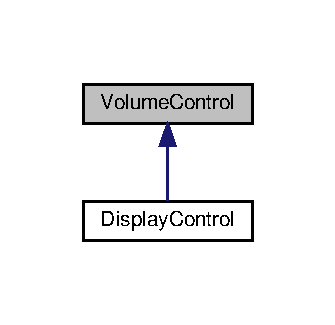
\includegraphics[width=161pt]{classVolumeControl__inherit__graph}
\end{center}
\end{figure}
\subsection*{Public Member Functions}
\begin{DoxyCompactItemize}
\item 
\hyperlink{classVolumeControl_a3cc73bb232bd87f8385da0440126c38c}{Volume\+Control} (void)
\item 
void \hyperlink{classVolumeControl_a6b51293368c1740b9bee0b8a4e7ed421}{increase\+Volume} ()
\item 
void \hyperlink{classVolumeControl_ad8e3e3740268388e906984fa807761a1}{reduce\+Volume} ()
\item 
void \hyperlink{classVolumeControl_a77273bc06d0f25068045860b0c6b4f91}{mute\+And\+Unmute} ()
\item 
void \hyperlink{classVolumeControl_a4a541c510e22cd07b206ca80f979c1a1}{unmute} ()
\end{DoxyCompactItemize}


\subsection{Detailed Description}
This class uses the A\+L\+SA library to send commands to the sound card. 

\subsection{Constructor \& Destructor Documentation}
\mbox{\Hypertarget{classVolumeControl_a3cc73bb232bd87f8385da0440126c38c}\label{classVolumeControl_a3cc73bb232bd87f8385da0440126c38c}} 
\index{Volume\+Control@{Volume\+Control}!Volume\+Control@{Volume\+Control}}
\index{Volume\+Control@{Volume\+Control}!Volume\+Control@{Volume\+Control}}
\subsubsection{\texorpdfstring{Volume\+Control()}{VolumeControl()}}
{\footnotesize\ttfamily Volume\+Control\+::\+Volume\+Control (\begin{DoxyParamCaption}\item[{void}]{ }\end{DoxyParamCaption})}

constructor 

\subsection{Member Function Documentation}
\mbox{\Hypertarget{classVolumeControl_a6b51293368c1740b9bee0b8a4e7ed421}\label{classVolumeControl_a6b51293368c1740b9bee0b8a4e7ed421}} 
\index{Volume\+Control@{Volume\+Control}!increase\+Volume@{increase\+Volume}}
\index{increase\+Volume@{increase\+Volume}!Volume\+Control@{Volume\+Control}}
\subsubsection{\texorpdfstring{increase\+Volume()}{increaseVolume()}}
{\footnotesize\ttfamily void Volume\+Control\+::increase\+Volume (\begin{DoxyParamCaption}{ }\end{DoxyParamCaption})}

Increase the master volume by 10\% \mbox{\Hypertarget{classVolumeControl_a77273bc06d0f25068045860b0c6b4f91}\label{classVolumeControl_a77273bc06d0f25068045860b0c6b4f91}} 
\index{Volume\+Control@{Volume\+Control}!mute\+And\+Unmute@{mute\+And\+Unmute}}
\index{mute\+And\+Unmute@{mute\+And\+Unmute}!Volume\+Control@{Volume\+Control}}
\subsubsection{\texorpdfstring{mute\+And\+Unmute()}{muteAndUnmute()}}
{\footnotesize\ttfamily void Volume\+Control\+::mute\+And\+Unmute (\begin{DoxyParamCaption}{ }\end{DoxyParamCaption})}

Mute or unmute by checking the current state. \mbox{\Hypertarget{classVolumeControl_ad8e3e3740268388e906984fa807761a1}\label{classVolumeControl_ad8e3e3740268388e906984fa807761a1}} 
\index{Volume\+Control@{Volume\+Control}!reduce\+Volume@{reduce\+Volume}}
\index{reduce\+Volume@{reduce\+Volume}!Volume\+Control@{Volume\+Control}}
\subsubsection{\texorpdfstring{reduce\+Volume()}{reduceVolume()}}
{\footnotesize\ttfamily void Volume\+Control\+::reduce\+Volume (\begin{DoxyParamCaption}{ }\end{DoxyParamCaption})}

Reduce the master volume by 10\% \mbox{\Hypertarget{classVolumeControl_a4a541c510e22cd07b206ca80f979c1a1}\label{classVolumeControl_a4a541c510e22cd07b206ca80f979c1a1}} 
\index{Volume\+Control@{Volume\+Control}!unmute@{unmute}}
\index{unmute@{unmute}!Volume\+Control@{Volume\+Control}}
\subsubsection{\texorpdfstring{unmute()}{unmute()}}
{\footnotesize\ttfamily void Volume\+Control\+::unmute (\begin{DoxyParamCaption}{ }\end{DoxyParamCaption})}

Umute the system, to be called before increases volume if system is muted. 

The documentation for this class was generated from the following files\+:\begin{DoxyCompactItemize}
\item 
src/ubuntu\+\_\+controls/\hyperlink{VolumeControl_8h}{Volume\+Control.\+h}\item 
src/ubuntu\+\_\+controls/\hyperlink{VolumeControl_8cpp}{Volume\+Control.\+cpp}\end{DoxyCompactItemize}

\hypertarget{classWindowAction}{}\section{Window\+Action Class Reference}
\label{classWindowAction}\index{Window\+Action@{Window\+Action}}


Contains functions that accessed by \hyperlink{classDisplayControl}{Display\+Control} to access the \hyperlink{classWindowControl}{Window\+Control}.  




{\ttfamily \#include $<$Window\+Action.\+h$>$}



Inheritance diagram for Window\+Action\+:\nopagebreak
\begin{figure}[H]
\begin{center}
\leavevmode
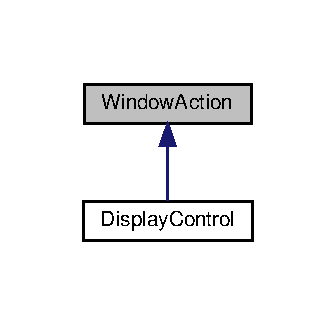
\includegraphics[width=161pt]{classWindowAction__inherit__graph}
\end{center}
\end{figure}
\subsection*{Public Member Functions}
\begin{DoxyCompactItemize}
\item 
\hyperlink{classWindowAction_a1836cf300ad545fa88f33454d09765e1}{Window\+Action} (Display $\ast$d)
\item 
void \hyperlink{classWindowAction_ac7145d79c3b902a716d554d09e6e2a63}{change\+Window\+Size} (int x, int y)
\item 
void \hyperlink{classWindowAction_ae79c374bbbc84ff3dfb8565ede5f4220}{move\+Window} (int x, int y)
\item 
void \hyperlink{classWindowAction_a99150ce49f2956c56e64b6ba0246424f}{close\+Window} ()
\item 
void \hyperlink{classWindowAction_aa6f2b2543505c0c44027b501f151d4bf}{minimize\+Window} ()
\end{DoxyCompactItemize}


\subsection{Detailed Description}
Contains functions that accessed by \hyperlink{classDisplayControl}{Display\+Control} to access the \hyperlink{classWindowControl}{Window\+Control}. 

\subsection{Constructor \& Destructor Documentation}
\mbox{\Hypertarget{classWindowAction_a1836cf300ad545fa88f33454d09765e1}\label{classWindowAction_a1836cf300ad545fa88f33454d09765e1}} 
\index{Window\+Action@{Window\+Action}!Window\+Action@{Window\+Action}}
\index{Window\+Action@{Window\+Action}!Window\+Action@{Window\+Action}}
\subsubsection{\texorpdfstring{Window\+Action()}{WindowAction()}}
{\footnotesize\ttfamily Window\+Action\+::\+Window\+Action (\begin{DoxyParamCaption}\item[{Display $\ast$}]{d }\end{DoxyParamCaption})}

constructor. 

\subsection{Member Function Documentation}
\mbox{\Hypertarget{classWindowAction_ac7145d79c3b902a716d554d09e6e2a63}\label{classWindowAction_ac7145d79c3b902a716d554d09e6e2a63}} 
\index{Window\+Action@{Window\+Action}!change\+Window\+Size@{change\+Window\+Size}}
\index{change\+Window\+Size@{change\+Window\+Size}!Window\+Action@{Window\+Action}}
\subsubsection{\texorpdfstring{change\+Window\+Size()}{changeWindowSize()}}
{\footnotesize\ttfamily void Window\+Action\+::change\+Window\+Size (\begin{DoxyParamCaption}\item[{int}]{x,  }\item[{int}]{y }\end{DoxyParamCaption})}

Call \hyperlink{classWindowControl}{Window\+Control} to change the size of the window (currently in development)


\begin{DoxyParams}{Parameters}
{\em x} & the x coordinate of the window \\
\hline
{\em y} & The y coordinate of the window. \\
\hline
\end{DoxyParams}
\mbox{\Hypertarget{classWindowAction_a99150ce49f2956c56e64b6ba0246424f}\label{classWindowAction_a99150ce49f2956c56e64b6ba0246424f}} 
\index{Window\+Action@{Window\+Action}!close\+Window@{close\+Window}}
\index{close\+Window@{close\+Window}!Window\+Action@{Window\+Action}}
\subsubsection{\texorpdfstring{close\+Window()}{closeWindow()}}
{\footnotesize\ttfamily void Window\+Action\+::close\+Window (\begin{DoxyParamCaption}{ }\end{DoxyParamCaption})}

Call \hyperlink{classWindowControl}{Window\+Control} to close the window (currently in development). \mbox{\Hypertarget{classWindowAction_aa6f2b2543505c0c44027b501f151d4bf}\label{classWindowAction_aa6f2b2543505c0c44027b501f151d4bf}} 
\index{Window\+Action@{Window\+Action}!minimize\+Window@{minimize\+Window}}
\index{minimize\+Window@{minimize\+Window}!Window\+Action@{Window\+Action}}
\subsubsection{\texorpdfstring{minimize\+Window()}{minimizeWindow()}}
{\footnotesize\ttfamily void Window\+Action\+::minimize\+Window (\begin{DoxyParamCaption}{ }\end{DoxyParamCaption})}

Call \hyperlink{classWindowControl}{Window\+Control} to minimize the window. \mbox{\Hypertarget{classWindowAction_ae79c374bbbc84ff3dfb8565ede5f4220}\label{classWindowAction_ae79c374bbbc84ff3dfb8565ede5f4220}} 
\index{Window\+Action@{Window\+Action}!move\+Window@{move\+Window}}
\index{move\+Window@{move\+Window}!Window\+Action@{Window\+Action}}
\subsubsection{\texorpdfstring{move\+Window()}{moveWindow()}}
{\footnotesize\ttfamily void Window\+Action\+::move\+Window (\begin{DoxyParamCaption}\item[{int}]{x,  }\item[{int}]{y }\end{DoxyParamCaption})}

Call \hyperlink{classWindowControl}{Window\+Control} to move the window to the specified coordinates.


\begin{DoxyParams}{Parameters}
{\em x} & The x coordinate of the window. \\
\hline
{\em y} & The y coordinate of the window. \\
\hline
\end{DoxyParams}


The documentation for this class was generated from the following files\+:\begin{DoxyCompactItemize}
\item 
src/ubuntu\+\_\+controls/\hyperlink{WindowAction_8h}{Window\+Action.\+h}\item 
src/ubuntu\+\_\+controls/\hyperlink{WindowAction_8cpp}{Window\+Action.\+cpp}\end{DoxyCompactItemize}

\hypertarget{classWindowControl}{}\section{Window\+Control Class Reference}
\label{classWindowControl}\index{Window\+Control@{Window\+Control}}


Used to send window events.  




{\ttfamily \#include $<$Window\+Control.\+h$>$}

\subsection*{Public Member Functions}
\begin{DoxyCompactItemize}
\item 
\hyperlink{classWindowControl_ac1737a56defaa8f60f53054b2167fee8}{Window\+Control} (void)
\item 
Window \hyperlink{classWindowControl_aad092a22b19664df4d94fe9a853d350a}{identify\+Window} (Display $\ast$display)
\item 
void \hyperlink{classWindowControl_a131a982c3338be4187ac6611591e042f}{resize} (Display $\ast$display, int x, int y)
\item 
void \hyperlink{classWindowControl_a367c48d4f217a83225c8ade45e347884}{move} (Display $\ast$display, int x, int y)
\item 
void \hyperlink{classWindowControl_abb8d0ae3c43be976259181c848fa4568}{minimize} (Display $\ast$display)
\item 
void \hyperlink{classWindowControl_a2f521062be8be113d1cbcca4f495d693}{close} (Display $\ast$display)
\end{DoxyCompactItemize}


\subsection{Detailed Description}
Used to send window events. 

\subsection{Constructor \& Destructor Documentation}
\mbox{\Hypertarget{classWindowControl_ac1737a56defaa8f60f53054b2167fee8}\label{classWindowControl_ac1737a56defaa8f60f53054b2167fee8}} 
\index{Window\+Control@{Window\+Control}!Window\+Control@{Window\+Control}}
\index{Window\+Control@{Window\+Control}!Window\+Control@{Window\+Control}}
\subsubsection{\texorpdfstring{Window\+Control()}{WindowControl()}}
{\footnotesize\ttfamily Window\+Control\+::\+Window\+Control (\begin{DoxyParamCaption}\item[{void}]{ }\end{DoxyParamCaption})}

Constructor 

\subsection{Member Function Documentation}
\mbox{\Hypertarget{classWindowControl_a2f521062be8be113d1cbcca4f495d693}\label{classWindowControl_a2f521062be8be113d1cbcca4f495d693}} 
\index{Window\+Control@{Window\+Control}!close@{close}}
\index{close@{close}!Window\+Control@{Window\+Control}}
\subsubsection{\texorpdfstring{close()}{close()}}
{\footnotesize\ttfamily void Window\+Control\+::close (\begin{DoxyParamCaption}\item[{Display $\ast$}]{display }\end{DoxyParamCaption})}

It closes the window


\begin{DoxyParams}{Parameters}
{\em display} & The display to use. \\
\hline
\end{DoxyParams}
\mbox{\Hypertarget{classWindowControl_aad092a22b19664df4d94fe9a853d350a}\label{classWindowControl_aad092a22b19664df4d94fe9a853d350a}} 
\index{Window\+Control@{Window\+Control}!identify\+Window@{identify\+Window}}
\index{identify\+Window@{identify\+Window}!Window\+Control@{Window\+Control}}
\subsubsection{\texorpdfstring{identify\+Window()}{identifyWindow()}}
{\footnotesize\ttfamily Window Window\+Control\+::identify\+Window (\begin{DoxyParamCaption}\item[{Display $\ast$}]{display }\end{DoxyParamCaption})}

It returns the window that currently has focus


\begin{DoxyParams}{Parameters}
{\em display} & The display to use.\\
\hline
\end{DoxyParams}
\begin{DoxyReturn}{Returns}
The window that has focus. 
\end{DoxyReturn}
\mbox{\Hypertarget{classWindowControl_abb8d0ae3c43be976259181c848fa4568}\label{classWindowControl_abb8d0ae3c43be976259181c848fa4568}} 
\index{Window\+Control@{Window\+Control}!minimize@{minimize}}
\index{minimize@{minimize}!Window\+Control@{Window\+Control}}
\subsubsection{\texorpdfstring{minimize()}{minimize()}}
{\footnotesize\ttfamily void Window\+Control\+::minimize (\begin{DoxyParamCaption}\item[{Display $\ast$}]{display }\end{DoxyParamCaption})}

It minimizes the window


\begin{DoxyParams}{Parameters}
{\em display} & The display to use. \\
\hline
\end{DoxyParams}
\mbox{\Hypertarget{classWindowControl_a367c48d4f217a83225c8ade45e347884}\label{classWindowControl_a367c48d4f217a83225c8ade45e347884}} 
\index{Window\+Control@{Window\+Control}!move@{move}}
\index{move@{move}!Window\+Control@{Window\+Control}}
\subsubsection{\texorpdfstring{move()}{move()}}
{\footnotesize\ttfamily void Window\+Control\+::move (\begin{DoxyParamCaption}\item[{Display $\ast$}]{display,  }\item[{int}]{x,  }\item[{int}]{y }\end{DoxyParamCaption})}

It moves the window to the specified coordinates


\begin{DoxyParams}{Parameters}
{\em display} & The display to use. \\
\hline
{\em x} & The x coordinate of the window\textquotesingle{}s new position. \\
\hline
{\em y} & The y coordinate of the window\textquotesingle{}s new position. \\
\hline
\end{DoxyParams}
\mbox{\Hypertarget{classWindowControl_a131a982c3338be4187ac6611591e042f}\label{classWindowControl_a131a982c3338be4187ac6611591e042f}} 
\index{Window\+Control@{Window\+Control}!resize@{resize}}
\index{resize@{resize}!Window\+Control@{Window\+Control}}
\subsubsection{\texorpdfstring{resize()}{resize()}}
{\footnotesize\ttfamily void Window\+Control\+::resize (\begin{DoxyParamCaption}\item[{Display $\ast$}]{display,  }\item[{int}]{x,  }\item[{int}]{y }\end{DoxyParamCaption})}

It takes a display and two integers as arguments, and resizes the window to the given dimensions


\begin{DoxyParams}{Parameters}
{\em display} & The display to use. \\
\hline
{\em x} & The x coordinate of the upper left corner of the window. \\
\hline
{\em y} & The y coordinate of the upper-\/left outside corner of the window. \\
\hline
\end{DoxyParams}


The documentation for this class was generated from the following files\+:\begin{DoxyCompactItemize}
\item 
src/ubuntu\+\_\+controls/\hyperlink{WindowControl_8h}{Window\+Control.\+h}\item 
src/ubuntu\+\_\+controls/\hyperlink{WindowControl_8cpp}{Window\+Control.\+cpp}\end{DoxyCompactItemize}

\chapter{File Documentation}
\hypertarget{README_8md}{}\section{R\+E\+A\+D\+M\+E.\+md File Reference}
\label{README_8md}\index{R\+E\+A\+D\+M\+E.\+md@{R\+E\+A\+D\+M\+E.\+md}}

\hypertarget{Capture_8cpp}{}\section{src/gesture\+\_\+detection/\+Capture.cpp File Reference}
\label{Capture_8cpp}\index{src/gesture\+\_\+detection/\+Capture.\+cpp@{src/gesture\+\_\+detection/\+Capture.\+cpp}}
{\ttfamily \#include \char`\"{}Capture.\+h\char`\"{}}\newline
Include dependency graph for Capture.\+cpp\+:\nopagebreak
\begin{figure}[H]
\begin{center}
\leavevmode
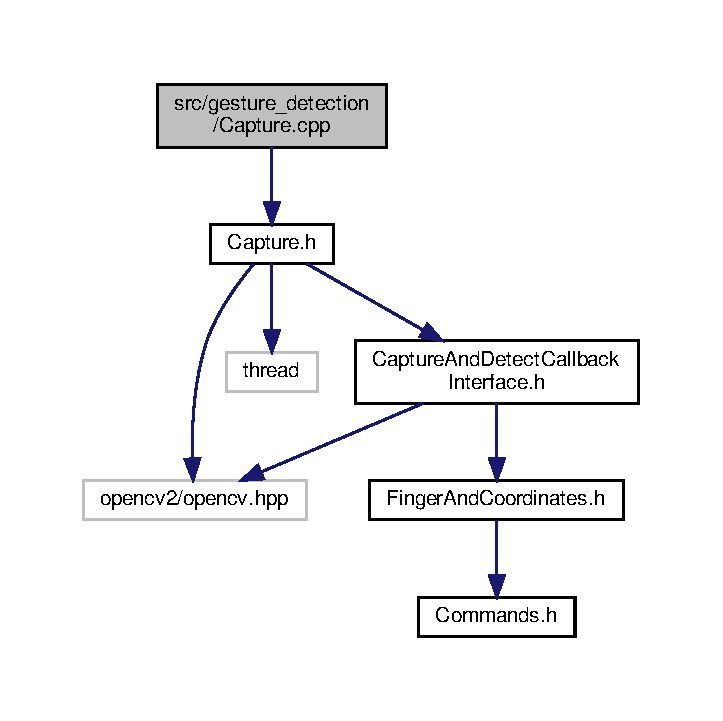
\includegraphics[width=347pt]{Capture_8cpp__incl}
\end{center}
\end{figure}

\hypertarget{Capture_8h}{}\section{src/gesture\+\_\+detection/\+Capture.h File Reference}
\label{Capture_8h}\index{src/gesture\+\_\+detection/\+Capture.\+h@{src/gesture\+\_\+detection/\+Capture.\+h}}
{\ttfamily \#include \char`\"{}opencv2/opencv.\+hpp\char`\"{}}\newline
{\ttfamily \#include $<$thread$>$}\newline
{\ttfamily \#include \char`\"{}Capture\+And\+Detect\+Callback\+Interface.\+h\char`\"{}}\newline
Include dependency graph for Capture.\+h\+:\nopagebreak
\begin{figure}[H]
\begin{center}
\leavevmode
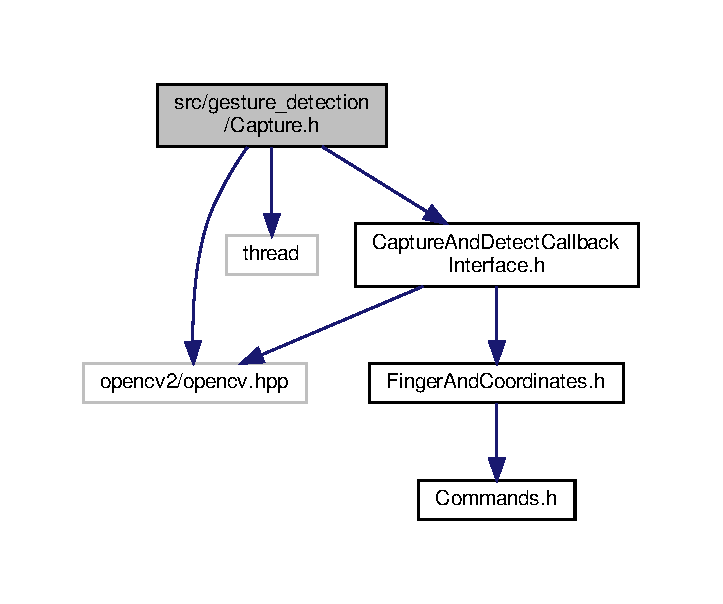
\includegraphics[width=347pt]{Capture_8h__incl}
\end{center}
\end{figure}
This graph shows which files directly or indirectly include this file\+:\nopagebreak
\begin{figure}[H]
\begin{center}
\leavevmode
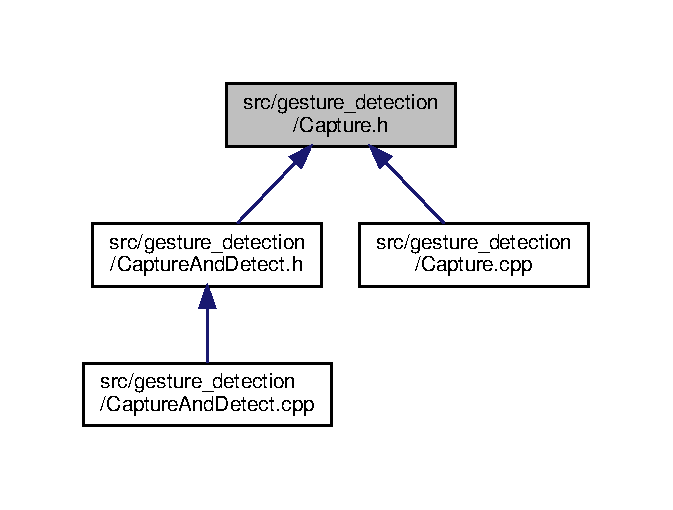
\includegraphics[width=323pt]{Capture_8h__dep__incl}
\end{center}
\end{figure}
\subsection*{Classes}
\begin{DoxyCompactItemize}
\item 
class \hyperlink{classCapture}{Capture}
\end{DoxyCompactItemize}

\hypertarget{CaptureAndDetect_8cpp}{}\section{src/gesture\+\_\+detection/\+Capture\+And\+Detect.cpp File Reference}
\label{CaptureAndDetect_8cpp}\index{src/gesture\+\_\+detection/\+Capture\+And\+Detect.\+cpp@{src/gesture\+\_\+detection/\+Capture\+And\+Detect.\+cpp}}
{\ttfamily \#include \char`\"{}Capture\+And\+Detect.\+h\char`\"{}}\newline
Include dependency graph for Capture\+And\+Detect.\+cpp\+:\nopagebreak
\begin{figure}[H]
\begin{center}
\leavevmode
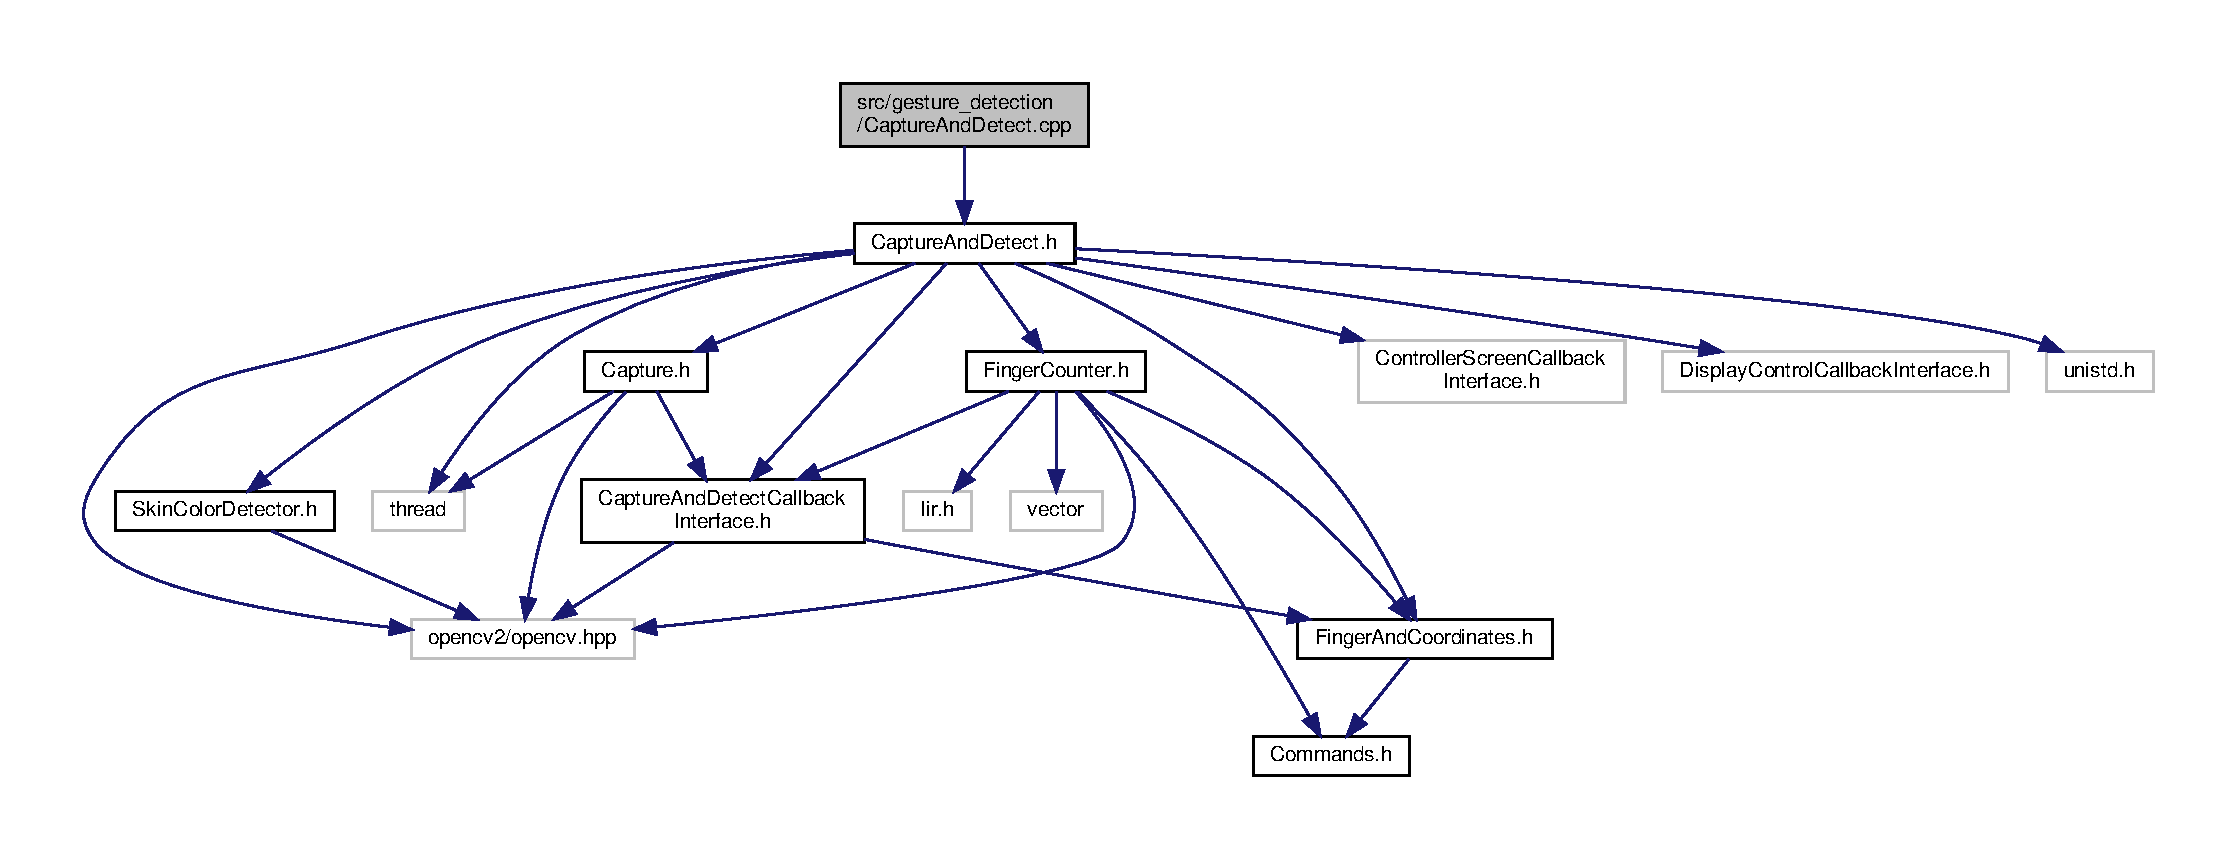
\includegraphics[width=350pt]{CaptureAndDetect_8cpp__incl}
\end{center}
\end{figure}

\hypertarget{CaptureAndDetect_8h}{}\section{src/gesture\+\_\+detection/\+Capture\+And\+Detect.h File Reference}
\label{CaptureAndDetect_8h}\index{src/gesture\+\_\+detection/\+Capture\+And\+Detect.\+h@{src/gesture\+\_\+detection/\+Capture\+And\+Detect.\+h}}
{\ttfamily \#include \char`\"{}opencv2/opencv.\+hpp\char`\"{}}\newline
{\ttfamily \#include \char`\"{}Skin\+Color\+Detector.\+h\char`\"{}}\newline
{\ttfamily \#include \char`\"{}Finger\+Counter.\+h\char`\"{}}\newline
{\ttfamily \#include \char`\"{}Finger\+And\+Coordinates.\+h\char`\"{}}\newline
{\ttfamily \#include \char`\"{}Capture.\+h\char`\"{}}\newline
{\ttfamily \#include \char`\"{}Controller\+Screen\+Callback\+Interface.\+h\char`\"{}}\newline
{\ttfamily \#include \char`\"{}Capture\+And\+Detect\+Callback\+Interface.\+h\char`\"{}}\newline
{\ttfamily \#include \char`\"{}Display\+Control\+Callback\+Interface.\+h\char`\"{}}\newline
{\ttfamily \#include \char`\"{}thread\char`\"{}}\newline
{\ttfamily \#include $<$unistd.\+h$>$}\newline
Include dependency graph for Capture\+And\+Detect.\+h\+:\nopagebreak
\begin{figure}[H]
\begin{center}
\leavevmode
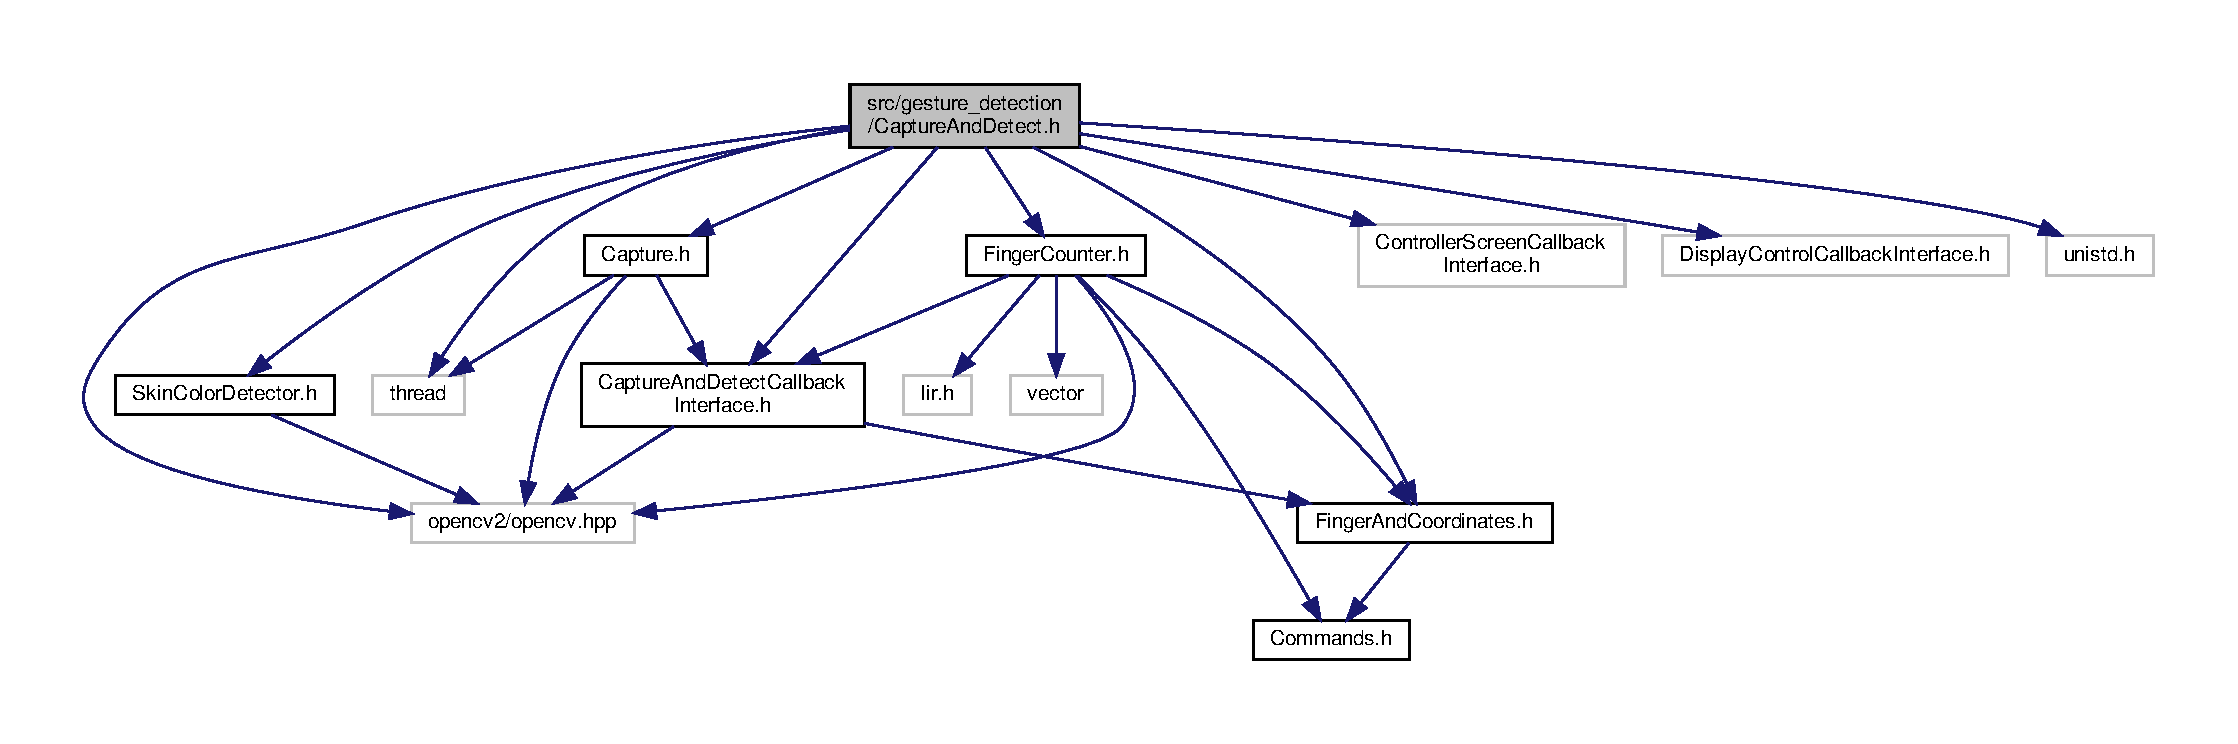
\includegraphics[width=350pt]{CaptureAndDetect_8h__incl}
\end{center}
\end{figure}
This graph shows which files directly or indirectly include this file\+:\nopagebreak
\begin{figure}[H]
\begin{center}
\leavevmode
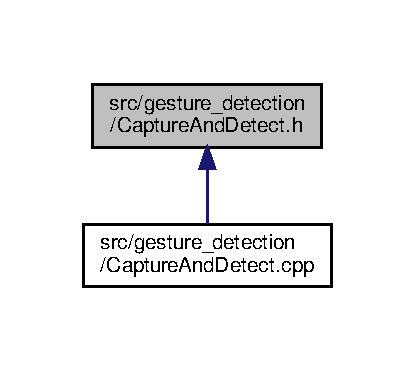
\includegraphics[width=199pt]{CaptureAndDetect_8h__dep__incl}
\end{center}
\end{figure}
\subsection*{Classes}
\begin{DoxyCompactItemize}
\item 
class \hyperlink{classGestro_1_1CaptureAndDetect}{Gestro\+::\+Capture\+And\+Detect}
\begin{DoxyCompactList}\small\item\em This class takes care of starting threads to capture image, process and publish commands. \end{DoxyCompactList}\end{DoxyCompactItemize}
\subsection*{Namespaces}
\begin{DoxyCompactItemize}
\item 
 \hyperlink{namespaceGestro}{Gestro}
\end{DoxyCompactItemize}
\subsection*{Enumerations}
\begin{DoxyCompactItemize}
\item 
enum \hyperlink{CaptureAndDetect_8h_a3c1fc1369ee351f25804c8cde5e85ac3}{Resolution} \{ \hyperlink{CaptureAndDetect_8h_a3c1fc1369ee351f25804c8cde5e85ac3a278580710dc7c233b4035c222f100b9f}{W\+I\+D\+T\+H\+\_\+1280} = 1280, 
\hyperlink{CaptureAndDetect_8h_a3c1fc1369ee351f25804c8cde5e85ac3aaf8940bab7f04c8cd702f61c4d051f27}{H\+E\+I\+G\+H\+T\+\_\+720} = 720, 
\hyperlink{CaptureAndDetect_8h_a3c1fc1369ee351f25804c8cde5e85ac3a62cb4c441f62ccfd155870b1d5e590d8}{W\+I\+D\+T\+H\+\_\+1920} = 1920, 
\hyperlink{CaptureAndDetect_8h_a3c1fc1369ee351f25804c8cde5e85ac3a62e4215c07636cf44ab26b46fabe7029}{H\+E\+I\+G\+H\+T\+\_\+1080} = 1080
 \}\begin{DoxyCompactList}\small\item\em enum to store resolution \end{DoxyCompactList}
\item 
enum \hyperlink{CaptureAndDetect_8h_a425a93be55e757f5e351ec9d6770c50e}{Feed} \{ \hyperlink{CaptureAndDetect_8h_a425a93be55e757f5e351ec9d6770c50ea93c33b647b7a4b7299c25e4e6d98ef7e}{U\+N\+P\+R\+O\+C\+E\+S\+S\+ED}, 
\hyperlink{CaptureAndDetect_8h_a425a93be55e757f5e351ec9d6770c50ea0c6d4f15b8bd03303ad52a8d155da661}{S\+K\+I\+N\+M\+A\+SK}, 
\hyperlink{CaptureAndDetect_8h_a425a93be55e757f5e351ec9d6770c50ead3560fe9fd615b5d3177bb08444bbe91}{D\+E\+T\+E\+C\+T\+ED}
 \}\begin{DoxyCompactList}\small\item\em enum for type of Feed \end{DoxyCompactList}
\end{DoxyCompactItemize}


\subsection{Enumeration Type Documentation}
\mbox{\Hypertarget{CaptureAndDetect_8h_a425a93be55e757f5e351ec9d6770c50e}\label{CaptureAndDetect_8h_a425a93be55e757f5e351ec9d6770c50e}} 
\index{Capture\+And\+Detect.\+h@{Capture\+And\+Detect.\+h}!Feed@{Feed}}
\index{Feed@{Feed}!Capture\+And\+Detect.\+h@{Capture\+And\+Detect.\+h}}
\subsubsection{\texorpdfstring{Feed}{Feed}}
{\footnotesize\ttfamily enum \hyperlink{CaptureAndDetect_8h_a425a93be55e757f5e351ec9d6770c50e}{Feed}}



enum for type of Feed 

\begin{DoxyEnumFields}{Enumerator}
\raisebox{\heightof{T}}[0pt][0pt]{\index{U\+N\+P\+R\+O\+C\+E\+S\+S\+ED@{U\+N\+P\+R\+O\+C\+E\+S\+S\+ED}!Capture\+And\+Detect.\+h@{Capture\+And\+Detect.\+h}}\index{Capture\+And\+Detect.\+h@{Capture\+And\+Detect.\+h}!U\+N\+P\+R\+O\+C\+E\+S\+S\+ED@{U\+N\+P\+R\+O\+C\+E\+S\+S\+ED}}}\mbox{\Hypertarget{CaptureAndDetect_8h_a425a93be55e757f5e351ec9d6770c50ea93c33b647b7a4b7299c25e4e6d98ef7e}\label{CaptureAndDetect_8h_a425a93be55e757f5e351ec9d6770c50ea93c33b647b7a4b7299c25e4e6d98ef7e}} 
U\+N\+P\+R\+O\+C\+E\+S\+S\+ED&\\
\hline

\raisebox{\heightof{T}}[0pt][0pt]{\index{S\+K\+I\+N\+M\+A\+SK@{S\+K\+I\+N\+M\+A\+SK}!Capture\+And\+Detect.\+h@{Capture\+And\+Detect.\+h}}\index{Capture\+And\+Detect.\+h@{Capture\+And\+Detect.\+h}!S\+K\+I\+N\+M\+A\+SK@{S\+K\+I\+N\+M\+A\+SK}}}\mbox{\Hypertarget{CaptureAndDetect_8h_a425a93be55e757f5e351ec9d6770c50ea0c6d4f15b8bd03303ad52a8d155da661}\label{CaptureAndDetect_8h_a425a93be55e757f5e351ec9d6770c50ea0c6d4f15b8bd03303ad52a8d155da661}} 
S\+K\+I\+N\+M\+A\+SK&\\
\hline

\raisebox{\heightof{T}}[0pt][0pt]{\index{D\+E\+T\+E\+C\+T\+ED@{D\+E\+T\+E\+C\+T\+ED}!Capture\+And\+Detect.\+h@{Capture\+And\+Detect.\+h}}\index{Capture\+And\+Detect.\+h@{Capture\+And\+Detect.\+h}!D\+E\+T\+E\+C\+T\+ED@{D\+E\+T\+E\+C\+T\+ED}}}\mbox{\Hypertarget{CaptureAndDetect_8h_a425a93be55e757f5e351ec9d6770c50ead3560fe9fd615b5d3177bb08444bbe91}\label{CaptureAndDetect_8h_a425a93be55e757f5e351ec9d6770c50ead3560fe9fd615b5d3177bb08444bbe91}} 
D\+E\+T\+E\+C\+T\+ED&\\
\hline

\end{DoxyEnumFields}
\mbox{\Hypertarget{CaptureAndDetect_8h_a3c1fc1369ee351f25804c8cde5e85ac3}\label{CaptureAndDetect_8h_a3c1fc1369ee351f25804c8cde5e85ac3}} 
\index{Capture\+And\+Detect.\+h@{Capture\+And\+Detect.\+h}!Resolution@{Resolution}}
\index{Resolution@{Resolution}!Capture\+And\+Detect.\+h@{Capture\+And\+Detect.\+h}}
\subsubsection{\texorpdfstring{Resolution}{Resolution}}
{\footnotesize\ttfamily enum \hyperlink{CaptureAndDetect_8h_a3c1fc1369ee351f25804c8cde5e85ac3}{Resolution}}



enum to store resolution 

\begin{DoxyEnumFields}{Enumerator}
\raisebox{\heightof{T}}[0pt][0pt]{\index{W\+I\+D\+T\+H\+\_\+1280@{W\+I\+D\+T\+H\+\_\+1280}!Capture\+And\+Detect.\+h@{Capture\+And\+Detect.\+h}}\index{Capture\+And\+Detect.\+h@{Capture\+And\+Detect.\+h}!W\+I\+D\+T\+H\+\_\+1280@{W\+I\+D\+T\+H\+\_\+1280}}}\mbox{\Hypertarget{CaptureAndDetect_8h_a3c1fc1369ee351f25804c8cde5e85ac3a278580710dc7c233b4035c222f100b9f}\label{CaptureAndDetect_8h_a3c1fc1369ee351f25804c8cde5e85ac3a278580710dc7c233b4035c222f100b9f}} 
W\+I\+D\+T\+H\+\_\+1280&\\
\hline

\raisebox{\heightof{T}}[0pt][0pt]{\index{H\+E\+I\+G\+H\+T\+\_\+720@{H\+E\+I\+G\+H\+T\+\_\+720}!Capture\+And\+Detect.\+h@{Capture\+And\+Detect.\+h}}\index{Capture\+And\+Detect.\+h@{Capture\+And\+Detect.\+h}!H\+E\+I\+G\+H\+T\+\_\+720@{H\+E\+I\+G\+H\+T\+\_\+720}}}\mbox{\Hypertarget{CaptureAndDetect_8h_a3c1fc1369ee351f25804c8cde5e85ac3aaf8940bab7f04c8cd702f61c4d051f27}\label{CaptureAndDetect_8h_a3c1fc1369ee351f25804c8cde5e85ac3aaf8940bab7f04c8cd702f61c4d051f27}} 
H\+E\+I\+G\+H\+T\+\_\+720&\\
\hline

\raisebox{\heightof{T}}[0pt][0pt]{\index{W\+I\+D\+T\+H\+\_\+1920@{W\+I\+D\+T\+H\+\_\+1920}!Capture\+And\+Detect.\+h@{Capture\+And\+Detect.\+h}}\index{Capture\+And\+Detect.\+h@{Capture\+And\+Detect.\+h}!W\+I\+D\+T\+H\+\_\+1920@{W\+I\+D\+T\+H\+\_\+1920}}}\mbox{\Hypertarget{CaptureAndDetect_8h_a3c1fc1369ee351f25804c8cde5e85ac3a62cb4c441f62ccfd155870b1d5e590d8}\label{CaptureAndDetect_8h_a3c1fc1369ee351f25804c8cde5e85ac3a62cb4c441f62ccfd155870b1d5e590d8}} 
W\+I\+D\+T\+H\+\_\+1920&\\
\hline

\raisebox{\heightof{T}}[0pt][0pt]{\index{H\+E\+I\+G\+H\+T\+\_\+1080@{H\+E\+I\+G\+H\+T\+\_\+1080}!Capture\+And\+Detect.\+h@{Capture\+And\+Detect.\+h}}\index{Capture\+And\+Detect.\+h@{Capture\+And\+Detect.\+h}!H\+E\+I\+G\+H\+T\+\_\+1080@{H\+E\+I\+G\+H\+T\+\_\+1080}}}\mbox{\Hypertarget{CaptureAndDetect_8h_a3c1fc1369ee351f25804c8cde5e85ac3a62e4215c07636cf44ab26b46fabe7029}\label{CaptureAndDetect_8h_a3c1fc1369ee351f25804c8cde5e85ac3a62e4215c07636cf44ab26b46fabe7029}} 
H\+E\+I\+G\+H\+T\+\_\+1080&\\
\hline

\end{DoxyEnumFields}

\hypertarget{CaptureAndDetectCallbackInterface_8h}{}\section{src/gesture\+\_\+detection/\+Capture\+And\+Detect\+Callback\+Interface.h File Reference}
\label{CaptureAndDetectCallbackInterface_8h}\index{src/gesture\+\_\+detection/\+Capture\+And\+Detect\+Callback\+Interface.\+h@{src/gesture\+\_\+detection/\+Capture\+And\+Detect\+Callback\+Interface.\+h}}
{\ttfamily \#include \char`\"{}opencv2/opencv.\+hpp\char`\"{}}\newline
{\ttfamily \#include \char`\"{}Finger\+And\+Coordinates.\+h\char`\"{}}\newline
Include dependency graph for Capture\+And\+Detect\+Callback\+Interface.\+h\+:\nopagebreak
\begin{figure}[H]
\begin{center}
\leavevmode
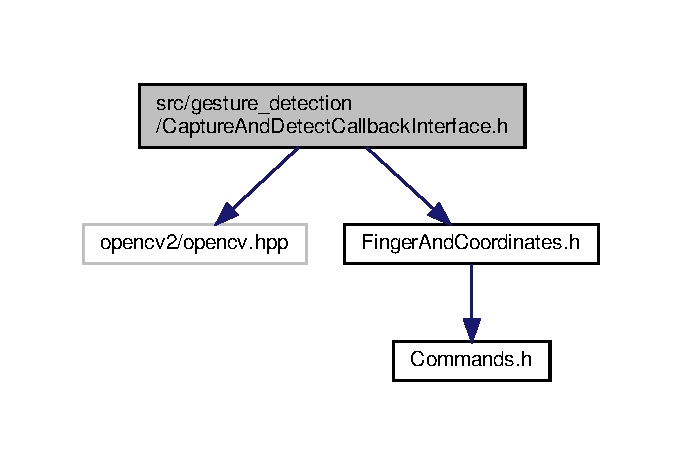
\includegraphics[width=328pt]{CaptureAndDetectCallbackInterface_8h__incl}
\end{center}
\end{figure}
This graph shows which files directly or indirectly include this file\+:\nopagebreak
\begin{figure}[H]
\begin{center}
\leavevmode
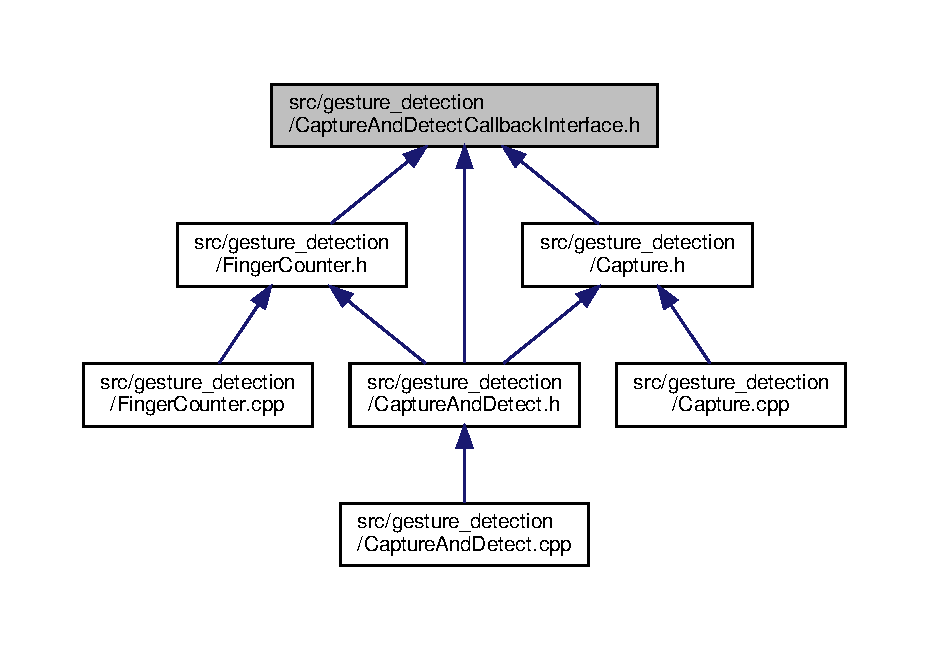
\includegraphics[width=350pt]{CaptureAndDetectCallbackInterface_8h__dep__incl}
\end{center}
\end{figure}
\subsection*{Classes}
\begin{DoxyCompactItemize}
\item 
class \hyperlink{classGestro_1_1CaptureAndDetectCallbackInterface}{Gestro\+::\+Capture\+And\+Detect\+Callback\+Interface}
\begin{DoxyCompactList}\small\item\em Callback interface for \hyperlink{classGestro_1_1CaptureAndDetect}{Capture\+And\+Detect}. \end{DoxyCompactList}\end{DoxyCompactItemize}
\subsection*{Namespaces}
\begin{DoxyCompactItemize}
\item 
 \hyperlink{namespaceGestro}{Gestro}
\end{DoxyCompactItemize}

\hypertarget{Commands_8h}{}\section{src/gesture\+\_\+detection/\+Commands.h File Reference}
\label{Commands_8h}\index{src/gesture\+\_\+detection/\+Commands.\+h@{src/gesture\+\_\+detection/\+Commands.\+h}}
This graph shows which files directly or indirectly include this file\+:\nopagebreak
\begin{figure}[H]
\begin{center}
\leavevmode
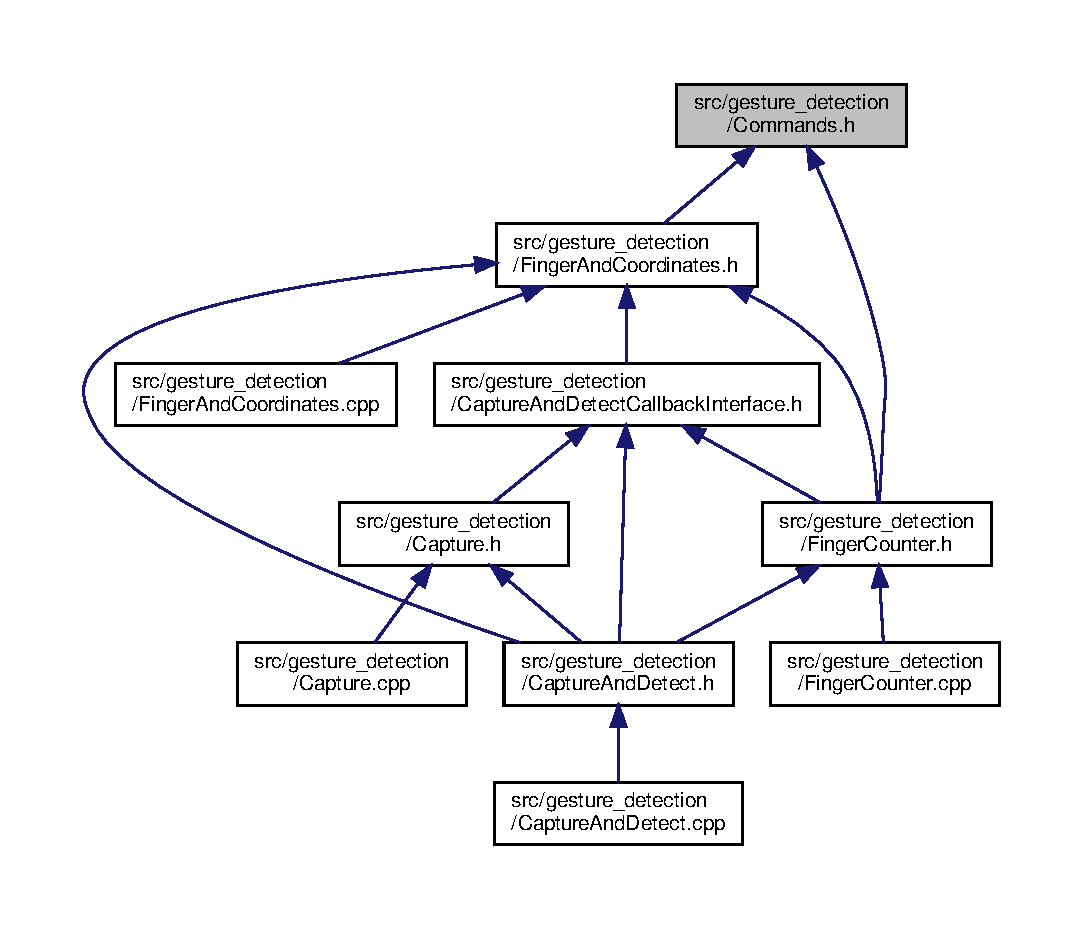
\includegraphics[width=350pt]{Commands_8h__dep__incl}
\end{center}
\end{figure}
\subsection*{Enumerations}
\begin{DoxyCompactItemize}
\item 
enum \hyperlink{Commands_8h_a1939e90743463fb34c8c571ec0590430}{Commands} \{ \newline
\hyperlink{Commands_8h_a1939e90743463fb34c8c571ec0590430ad60fa75796b89a3bfd5d4c1798499c90}{N\+O\+\_\+\+F\+I\+N\+G\+ER}, 
\hyperlink{Commands_8h_a1939e90743463fb34c8c571ec0590430a7513d383f97428a41f8b44594874d469}{M\+O\+U\+S\+E\+\_\+\+M\+O\+VE}, 
\hyperlink{Commands_8h_a1939e90743463fb34c8c571ec0590430a6e5c89c351b7128fdba923464fcdb47a}{M\+O\+U\+S\+E\+\_\+\+C\+L\+I\+CK}, 
\hyperlink{Commands_8h_a1939e90743463fb34c8c571ec0590430a9a06e9be8a466cb25472fc5d2245adc2}{V\+O\+L\+U\+M\+E\+\_\+\+UP}, 
\newline
\hyperlink{Commands_8h_a1939e90743463fb34c8c571ec0590430a529d2dedd2400b280c220d9892527bc7}{V\+O\+L\+U\+M\+E\+\_\+\+D\+O\+WN}, 
\hyperlink{Commands_8h_a1939e90743463fb34c8c571ec0590430a512f4445bc4a96f8e9714ecae8440b35}{M\+U\+T\+E\+\_\+\+U\+N\+M\+U\+TE}, 
\hyperlink{Commands_8h_a1939e90743463fb34c8c571ec0590430a8da4f522968e4f3f86e96bb8c91551c5}{M\+O\+V\+E\+\_\+\+W\+I\+N\+D\+OW}, 
\hyperlink{Commands_8h_a1939e90743463fb34c8c571ec0590430a91e132cc77d496b33c233c6381ddf12e}{M\+I\+N\+I\+M\+I\+Z\+E\+\_\+\+W\+I\+N\+D\+OW}, 
\newline
\hyperlink{Commands_8h_a1939e90743463fb34c8c571ec0590430ae32039d3fd427fe4b88245ab88126722}{P\+R\+E\+S\+S\+\_\+\+S\+P\+A\+CE}
 \}\begin{DoxyCompactList}\small\item\em Defining a list of commands that can be used in the program. \end{DoxyCompactList}
\end{DoxyCompactItemize}


\subsection{Enumeration Type Documentation}
\mbox{\Hypertarget{Commands_8h_a1939e90743463fb34c8c571ec0590430}\label{Commands_8h_a1939e90743463fb34c8c571ec0590430}} 
\index{Commands.\+h@{Commands.\+h}!Commands@{Commands}}
\index{Commands@{Commands}!Commands.\+h@{Commands.\+h}}
\subsubsection{\texorpdfstring{Commands}{Commands}}
{\footnotesize\ttfamily enum \hyperlink{Commands_8h_a1939e90743463fb34c8c571ec0590430}{Commands}}



Defining a list of commands that can be used in the program. 

\begin{DoxyEnumFields}{Enumerator}
\raisebox{\heightof{T}}[0pt][0pt]{\index{N\+O\+\_\+\+F\+I\+N\+G\+ER@{N\+O\+\_\+\+F\+I\+N\+G\+ER}!Commands.\+h@{Commands.\+h}}\index{Commands.\+h@{Commands.\+h}!N\+O\+\_\+\+F\+I\+N\+G\+ER@{N\+O\+\_\+\+F\+I\+N\+G\+ER}}}\mbox{\Hypertarget{Commands_8h_a1939e90743463fb34c8c571ec0590430ad60fa75796b89a3bfd5d4c1798499c90}\label{Commands_8h_a1939e90743463fb34c8c571ec0590430ad60fa75796b89a3bfd5d4c1798499c90}} 
N\+O\+\_\+\+F\+I\+N\+G\+ER&Used to indicate that there is no finger detected. \\
\hline

\raisebox{\heightof{T}}[0pt][0pt]{\index{M\+O\+U\+S\+E\+\_\+\+M\+O\+VE@{M\+O\+U\+S\+E\+\_\+\+M\+O\+VE}!Commands.\+h@{Commands.\+h}}\index{Commands.\+h@{Commands.\+h}!M\+O\+U\+S\+E\+\_\+\+M\+O\+VE@{M\+O\+U\+S\+E\+\_\+\+M\+O\+VE}}}\mbox{\Hypertarget{Commands_8h_a1939e90743463fb34c8c571ec0590430a7513d383f97428a41f8b44594874d469}\label{Commands_8h_a1939e90743463fb34c8c571ec0590430a7513d383f97428a41f8b44594874d469}} 
M\+O\+U\+S\+E\+\_\+\+M\+O\+VE&Command to move the mouse \\
\hline

\raisebox{\heightof{T}}[0pt][0pt]{\index{M\+O\+U\+S\+E\+\_\+\+C\+L\+I\+CK@{M\+O\+U\+S\+E\+\_\+\+C\+L\+I\+CK}!Commands.\+h@{Commands.\+h}}\index{Commands.\+h@{Commands.\+h}!M\+O\+U\+S\+E\+\_\+\+C\+L\+I\+CK@{M\+O\+U\+S\+E\+\_\+\+C\+L\+I\+CK}}}\mbox{\Hypertarget{Commands_8h_a1939e90743463fb34c8c571ec0590430a6e5c89c351b7128fdba923464fcdb47a}\label{Commands_8h_a1939e90743463fb34c8c571ec0590430a6e5c89c351b7128fdba923464fcdb47a}} 
M\+O\+U\+S\+E\+\_\+\+C\+L\+I\+CK&Mouse Click Occured \\
\hline

\raisebox{\heightof{T}}[0pt][0pt]{\index{V\+O\+L\+U\+M\+E\+\_\+\+UP@{V\+O\+L\+U\+M\+E\+\_\+\+UP}!Commands.\+h@{Commands.\+h}}\index{Commands.\+h@{Commands.\+h}!V\+O\+L\+U\+M\+E\+\_\+\+UP@{V\+O\+L\+U\+M\+E\+\_\+\+UP}}}\mbox{\Hypertarget{Commands_8h_a1939e90743463fb34c8c571ec0590430a9a06e9be8a466cb25472fc5d2245adc2}\label{Commands_8h_a1939e90743463fb34c8c571ec0590430a9a06e9be8a466cb25472fc5d2245adc2}} 
V\+O\+L\+U\+M\+E\+\_\+\+UP&Increase Volume \\
\hline

\raisebox{\heightof{T}}[0pt][0pt]{\index{V\+O\+L\+U\+M\+E\+\_\+\+D\+O\+WN@{V\+O\+L\+U\+M\+E\+\_\+\+D\+O\+WN}!Commands.\+h@{Commands.\+h}}\index{Commands.\+h@{Commands.\+h}!V\+O\+L\+U\+M\+E\+\_\+\+D\+O\+WN@{V\+O\+L\+U\+M\+E\+\_\+\+D\+O\+WN}}}\mbox{\Hypertarget{Commands_8h_a1939e90743463fb34c8c571ec0590430a529d2dedd2400b280c220d9892527bc7}\label{Commands_8h_a1939e90743463fb34c8c571ec0590430a529d2dedd2400b280c220d9892527bc7}} 
V\+O\+L\+U\+M\+E\+\_\+\+D\+O\+WN&Decrease Volume \\
\hline

\raisebox{\heightof{T}}[0pt][0pt]{\index{M\+U\+T\+E\+\_\+\+U\+N\+M\+U\+TE@{M\+U\+T\+E\+\_\+\+U\+N\+M\+U\+TE}!Commands.\+h@{Commands.\+h}}\index{Commands.\+h@{Commands.\+h}!M\+U\+T\+E\+\_\+\+U\+N\+M\+U\+TE@{M\+U\+T\+E\+\_\+\+U\+N\+M\+U\+TE}}}\mbox{\Hypertarget{Commands_8h_a1939e90743463fb34c8c571ec0590430a512f4445bc4a96f8e9714ecae8440b35}\label{Commands_8h_a1939e90743463fb34c8c571ec0590430a512f4445bc4a96f8e9714ecae8440b35}} 
M\+U\+T\+E\+\_\+\+U\+N\+M\+U\+TE&Mute and Unmute the volume \\
\hline

\raisebox{\heightof{T}}[0pt][0pt]{\index{M\+O\+V\+E\+\_\+\+W\+I\+N\+D\+OW@{M\+O\+V\+E\+\_\+\+W\+I\+N\+D\+OW}!Commands.\+h@{Commands.\+h}}\index{Commands.\+h@{Commands.\+h}!M\+O\+V\+E\+\_\+\+W\+I\+N\+D\+OW@{M\+O\+V\+E\+\_\+\+W\+I\+N\+D\+OW}}}\mbox{\Hypertarget{Commands_8h_a1939e90743463fb34c8c571ec0590430a8da4f522968e4f3f86e96bb8c91551c5}\label{Commands_8h_a1939e90743463fb34c8c571ec0590430a8da4f522968e4f3f86e96bb8c91551c5}} 
M\+O\+V\+E\+\_\+\+W\+I\+N\+D\+OW&Move the window \\
\hline

\raisebox{\heightof{T}}[0pt][0pt]{\index{M\+I\+N\+I\+M\+I\+Z\+E\+\_\+\+W\+I\+N\+D\+OW@{M\+I\+N\+I\+M\+I\+Z\+E\+\_\+\+W\+I\+N\+D\+OW}!Commands.\+h@{Commands.\+h}}\index{Commands.\+h@{Commands.\+h}!M\+I\+N\+I\+M\+I\+Z\+E\+\_\+\+W\+I\+N\+D\+OW@{M\+I\+N\+I\+M\+I\+Z\+E\+\_\+\+W\+I\+N\+D\+OW}}}\mbox{\Hypertarget{Commands_8h_a1939e90743463fb34c8c571ec0590430a91e132cc77d496b33c233c6381ddf12e}\label{Commands_8h_a1939e90743463fb34c8c571ec0590430a91e132cc77d496b33c233c6381ddf12e}} 
M\+I\+N\+I\+M\+I\+Z\+E\+\_\+\+W\+I\+N\+D\+OW&Minimize the window \\
\hline

\raisebox{\heightof{T}}[0pt][0pt]{\index{P\+R\+E\+S\+S\+\_\+\+S\+P\+A\+CE@{P\+R\+E\+S\+S\+\_\+\+S\+P\+A\+CE}!Commands.\+h@{Commands.\+h}}\index{Commands.\+h@{Commands.\+h}!P\+R\+E\+S\+S\+\_\+\+S\+P\+A\+CE@{P\+R\+E\+S\+S\+\_\+\+S\+P\+A\+CE}}}\mbox{\Hypertarget{Commands_8h_a1939e90743463fb34c8c571ec0590430ae32039d3fd427fe4b88245ab88126722}\label{Commands_8h_a1939e90743463fb34c8c571ec0590430ae32039d3fd427fe4b88245ab88126722}} 
P\+R\+E\+S\+S\+\_\+\+S\+P\+A\+CE&Press space bar \\
\hline

\end{DoxyEnumFields}

\hypertarget{FingerAndCoordinates_8cpp}{}\section{src/gesture\+\_\+detection/\+Finger\+And\+Coordinates.cpp File Reference}
\label{FingerAndCoordinates_8cpp}\index{src/gesture\+\_\+detection/\+Finger\+And\+Coordinates.\+cpp@{src/gesture\+\_\+detection/\+Finger\+And\+Coordinates.\+cpp}}
{\ttfamily \#include \char`\"{}Finger\+And\+Coordinates.\+h\char`\"{}}\newline
Include dependency graph for Finger\+And\+Coordinates.\+cpp\+:\nopagebreak
\begin{figure}[H]
\begin{center}
\leavevmode
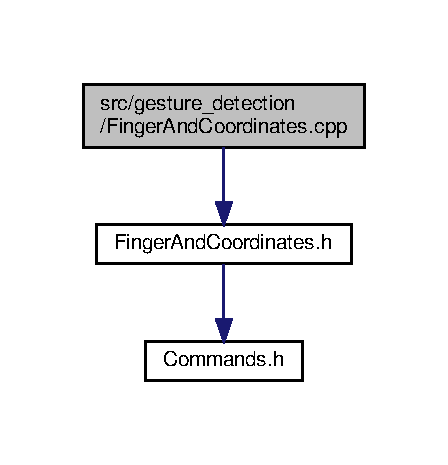
\includegraphics[width=215pt]{FingerAndCoordinates_8cpp__incl}
\end{center}
\end{figure}

\hypertarget{FingerAndCoordinates_8h}{}\section{src/gesture\+\_\+detection/\+Finger\+And\+Coordinates.h File Reference}
\label{FingerAndCoordinates_8h}\index{src/gesture\+\_\+detection/\+Finger\+And\+Coordinates.\+h@{src/gesture\+\_\+detection/\+Finger\+And\+Coordinates.\+h}}
{\ttfamily \#include \char`\"{}Commands.\+h\char`\"{}}\newline
Include dependency graph for Finger\+And\+Coordinates.\+h\+:\nopagebreak
\begin{figure}[H]
\begin{center}
\leavevmode
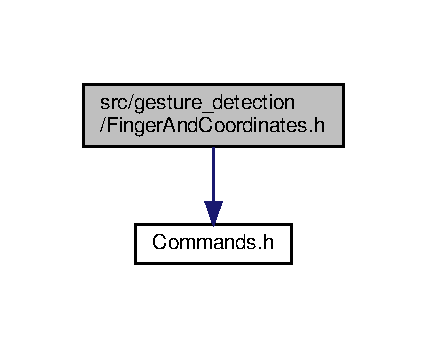
\includegraphics[width=205pt]{FingerAndCoordinates_8h__incl}
\end{center}
\end{figure}
This graph shows which files directly or indirectly include this file\+:\nopagebreak
\begin{figure}[H]
\begin{center}
\leavevmode
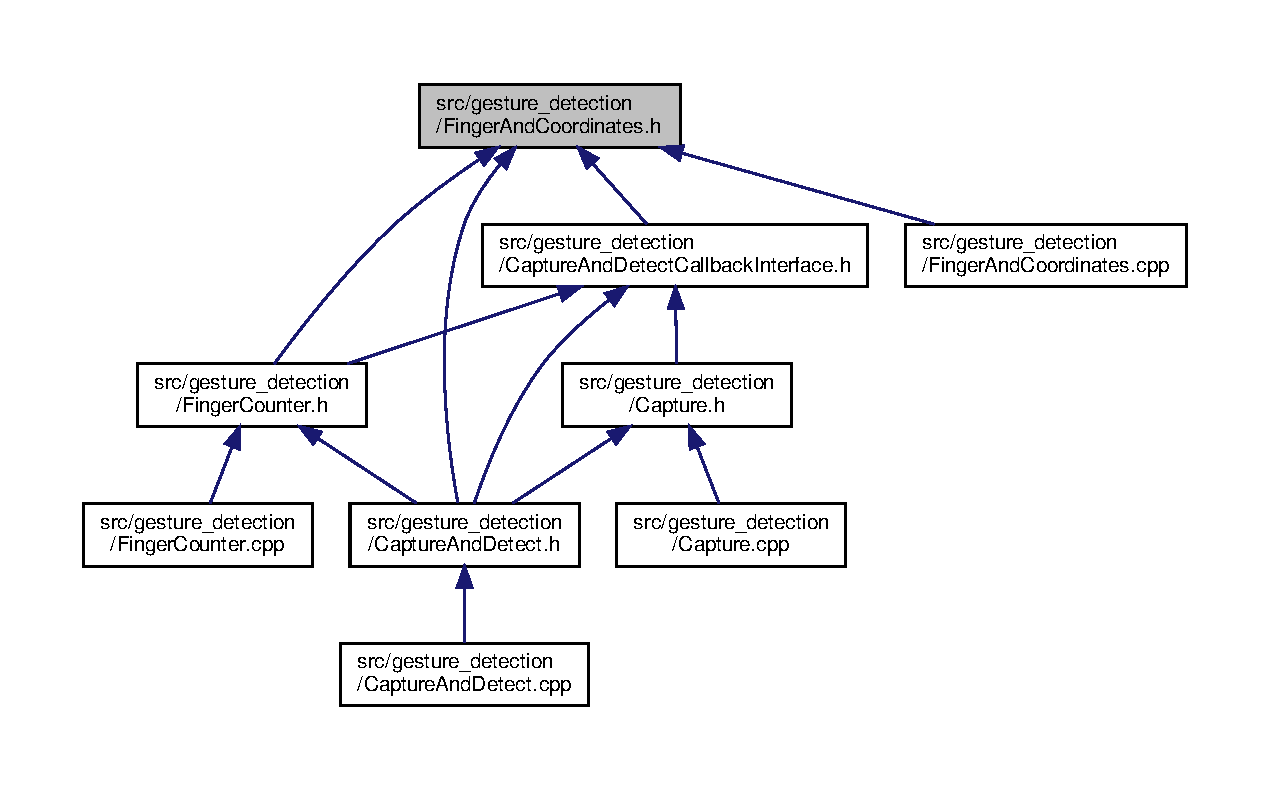
\includegraphics[width=350pt]{FingerAndCoordinates_8h__dep__incl}
\end{center}
\end{figure}
\subsection*{Classes}
\begin{DoxyCompactItemize}
\item 
class \hyperlink{classGestureDetection_1_1FingerAndCoordinates}{Gesture\+Detection\+::\+Finger\+And\+Coordinates}
\begin{DoxyCompactList}\small\item\em class to store the information detected by the \hyperlink{classGestureDetection_1_1FingerCounter}{Finger\+Counter}. \end{DoxyCompactList}\end{DoxyCompactItemize}
\subsection*{Namespaces}
\begin{DoxyCompactItemize}
\item 
 \hyperlink{namespaceGestureDetection}{Gesture\+Detection}
\end{DoxyCompactItemize}

\hypertarget{FingerCounter_8cpp}{}\section{src/gesture\+\_\+detection/\+Finger\+Counter.cpp File Reference}
\label{FingerCounter_8cpp}\index{src/gesture\+\_\+detection/\+Finger\+Counter.\+cpp@{src/gesture\+\_\+detection/\+Finger\+Counter.\+cpp}}
{\ttfamily \#include \char`\"{}Finger\+Counter.\+h\char`\"{}}\newline
Include dependency graph for Finger\+Counter.\+cpp\+:\nopagebreak
\begin{figure}[H]
\begin{center}
\leavevmode
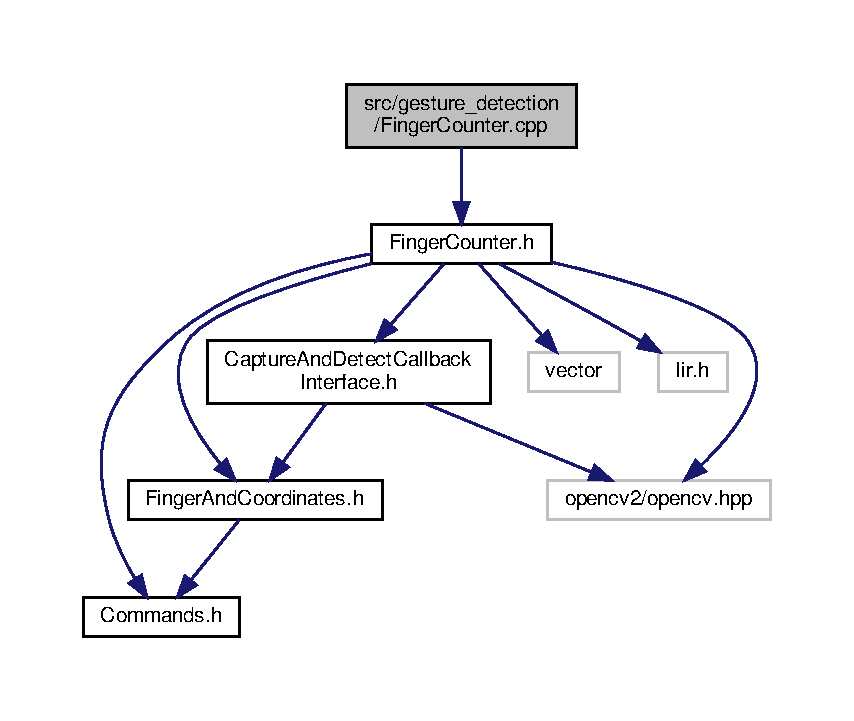
\includegraphics[width=350pt]{FingerCounter_8cpp__incl}
\end{center}
\end{figure}

\hypertarget{FingerCounter_8h}{}\section{src/gesture\+\_\+detection/\+Finger\+Counter.h File Reference}
\label{FingerCounter_8h}\index{src/gesture\+\_\+detection/\+Finger\+Counter.\+h@{src/gesture\+\_\+detection/\+Finger\+Counter.\+h}}
{\ttfamily \#include \char`\"{}Finger\+And\+Coordinates.\+h\char`\"{}}\newline
{\ttfamily \#include \char`\"{}opencv2/opencv.\+hpp\char`\"{}}\newline
{\ttfamily \#include \char`\"{}vector\char`\"{}}\newline
{\ttfamily \#include \char`\"{}Iir.\+h\char`\"{}}\newline
{\ttfamily \#include \char`\"{}Capture\+And\+Detect\+Callback\+Interface.\+h\char`\"{}}\newline
{\ttfamily \#include \char`\"{}Commands.\+h\char`\"{}}\newline
Include dependency graph for Finger\+Counter.\+h\+:\nopagebreak
\begin{figure}[H]
\begin{center}
\leavevmode
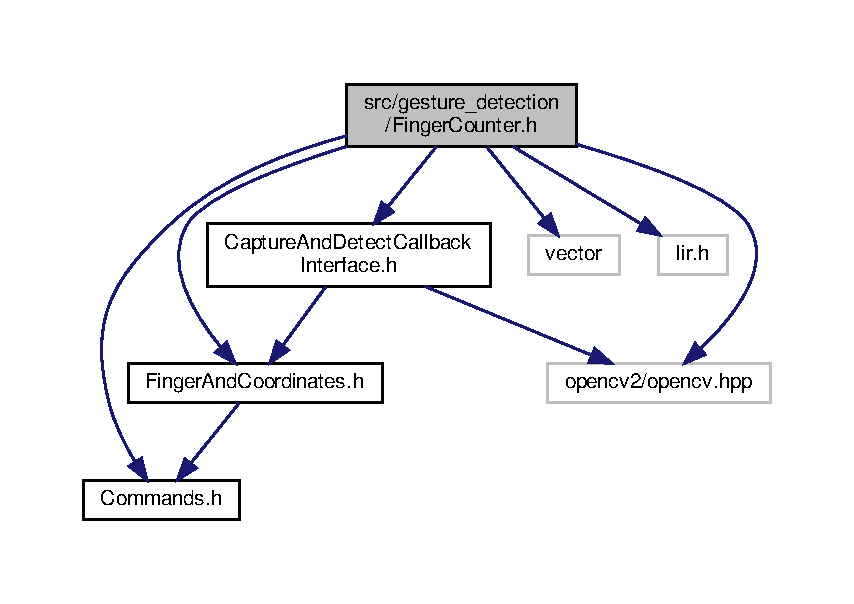
\includegraphics[width=350pt]{FingerCounter_8h__incl}
\end{center}
\end{figure}
This graph shows which files directly or indirectly include this file\+:\nopagebreak
\begin{figure}[H]
\begin{center}
\leavevmode
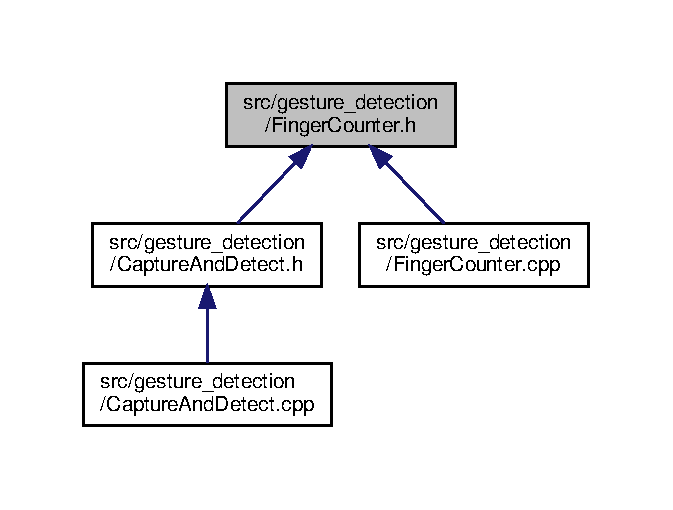
\includegraphics[width=323pt]{FingerCounter_8h__dep__incl}
\end{center}
\end{figure}
\subsection*{Classes}
\begin{DoxyCompactItemize}
\item 
class \hyperlink{classGestureDetection_1_1FingerCounter}{Gesture\+Detection\+::\+Finger\+Counter}
\begin{DoxyCompactList}\small\item\em checks the number of fingers and sends the respective command to be processed. \end{DoxyCompactList}\end{DoxyCompactItemize}
\subsection*{Namespaces}
\begin{DoxyCompactItemize}
\item 
 \hyperlink{namespaceGestureDetection}{Gesture\+Detection}
\end{DoxyCompactItemize}

\hypertarget{SkinColorDetector_8cpp}{}\section{src/gesture\+\_\+detection/\+Skin\+Color\+Detector.cpp File Reference}
\label{SkinColorDetector_8cpp}\index{src/gesture\+\_\+detection/\+Skin\+Color\+Detector.\+cpp@{src/gesture\+\_\+detection/\+Skin\+Color\+Detector.\+cpp}}
{\ttfamily \#include \char`\"{}Skin\+Color\+Detector.\+h\char`\"{}}\newline
Include dependency graph for Skin\+Color\+Detector.\+cpp\+:\nopagebreak
\begin{figure}[H]
\begin{center}
\leavevmode
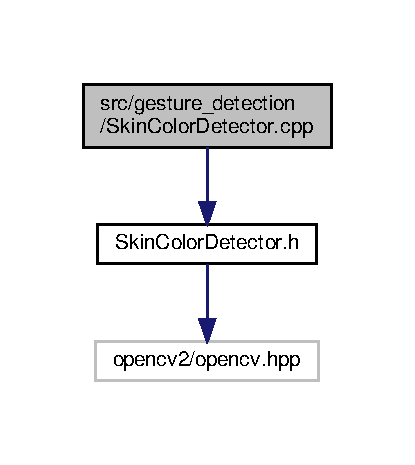
\includegraphics[width=199pt]{SkinColorDetector_8cpp__incl}
\end{center}
\end{figure}

\hypertarget{SkinColorDetector_8h}{}\section{src/gesture\+\_\+detection/\+Skin\+Color\+Detector.h File Reference}
\label{SkinColorDetector_8h}\index{src/gesture\+\_\+detection/\+Skin\+Color\+Detector.\+h@{src/gesture\+\_\+detection/\+Skin\+Color\+Detector.\+h}}
{\ttfamily \#include \char`\"{}opencv2/opencv.\+hpp\char`\"{}}\newline
Include dependency graph for Skin\+Color\+Detector.\+h\+:\nopagebreak
\begin{figure}[H]
\begin{center}
\leavevmode
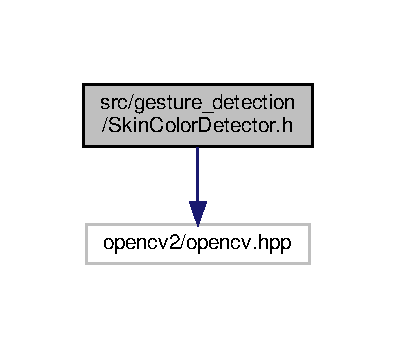
\includegraphics[width=190pt]{SkinColorDetector_8h__incl}
\end{center}
\end{figure}
This graph shows which files directly or indirectly include this file\+:\nopagebreak
\begin{figure}[H]
\begin{center}
\leavevmode
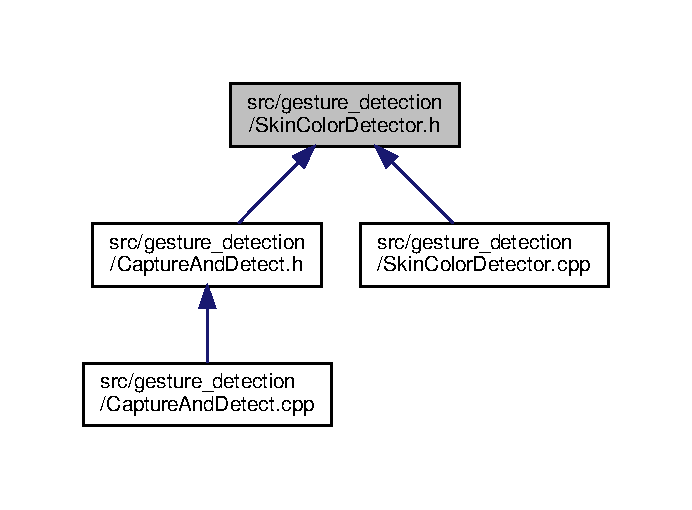
\includegraphics[width=332pt]{SkinColorDetector_8h__dep__incl}
\end{center}
\end{figure}
\subsection*{Classes}
\begin{DoxyCompactItemize}
\item 
class \hyperlink{classSkinColorDetector}{Skin\+Color\+Detector}
\begin{DoxyCompactList}\small\item\em detects skin colour threshold and creates a skin mask. \end{DoxyCompactList}\end{DoxyCompactItemize}

\hypertarget{main_8cpp}{}\section{src/main.cpp File Reference}
\label{main_8cpp}\index{src/main.\+cpp@{src/main.\+cpp}}
{\ttfamily \#include \char`\"{}gui/\+Start\+Screen.\+h\char`\"{}}\newline
{\ttfamily \#include \char`\"{}Q\+Application\char`\"{}}\newline
Include dependency graph for main.\+cpp\+:
\nopagebreak
\begin{figure}[H]
\begin{center}
\leavevmode
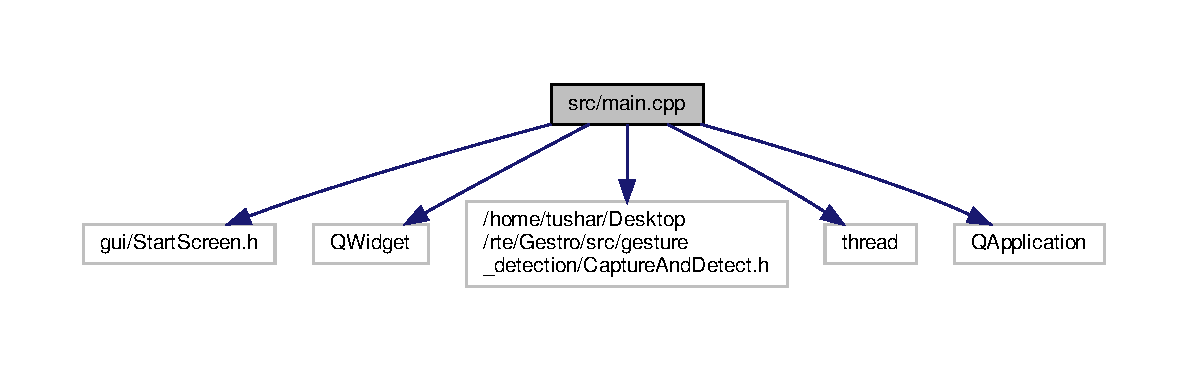
\includegraphics[width=350pt]{main_8cpp__incl}
\end{center}
\end{figure}
\subsection*{Functions}
\begin{DoxyCompactItemize}
\item 
int \hyperlink{main_8cpp_a0ddf1224851353fc92bfbff6f499fa97}{main} (int argc, char $\ast$argv\mbox{[}$\,$\mbox{]})
\end{DoxyCompactItemize}


\subsection{Function Documentation}
\mbox{\Hypertarget{main_8cpp_a0ddf1224851353fc92bfbff6f499fa97}\label{main_8cpp_a0ddf1224851353fc92bfbff6f499fa97}} 
\index{main.\+cpp@{main.\+cpp}!main@{main}}
\index{main@{main}!main.\+cpp@{main.\+cpp}}
\subsubsection{\texorpdfstring{main()}{main()}}
{\footnotesize\ttfamily int main (\begin{DoxyParamCaption}\item[{int}]{argc,  }\item[{char $\ast$}]{argv\mbox{[}$\,$\mbox{]} }\end{DoxyParamCaption})}



Definition at line 6 of file main.\+cpp.


\hypertarget{DisplayControl_8cpp}{}\section{src/ubuntu\+\_\+controls/\+Display\+Control.cpp File Reference}
\label{DisplayControl_8cpp}\index{src/ubuntu\+\_\+controls/\+Display\+Control.\+cpp@{src/ubuntu\+\_\+controls/\+Display\+Control.\+cpp}}
{\ttfamily \#include \char`\"{}Display\+Control.\+h\char`\"{}}\newline
Include dependency graph for Display\+Control.\+cpp\+:\nopagebreak
\begin{figure}[H]
\begin{center}
\leavevmode
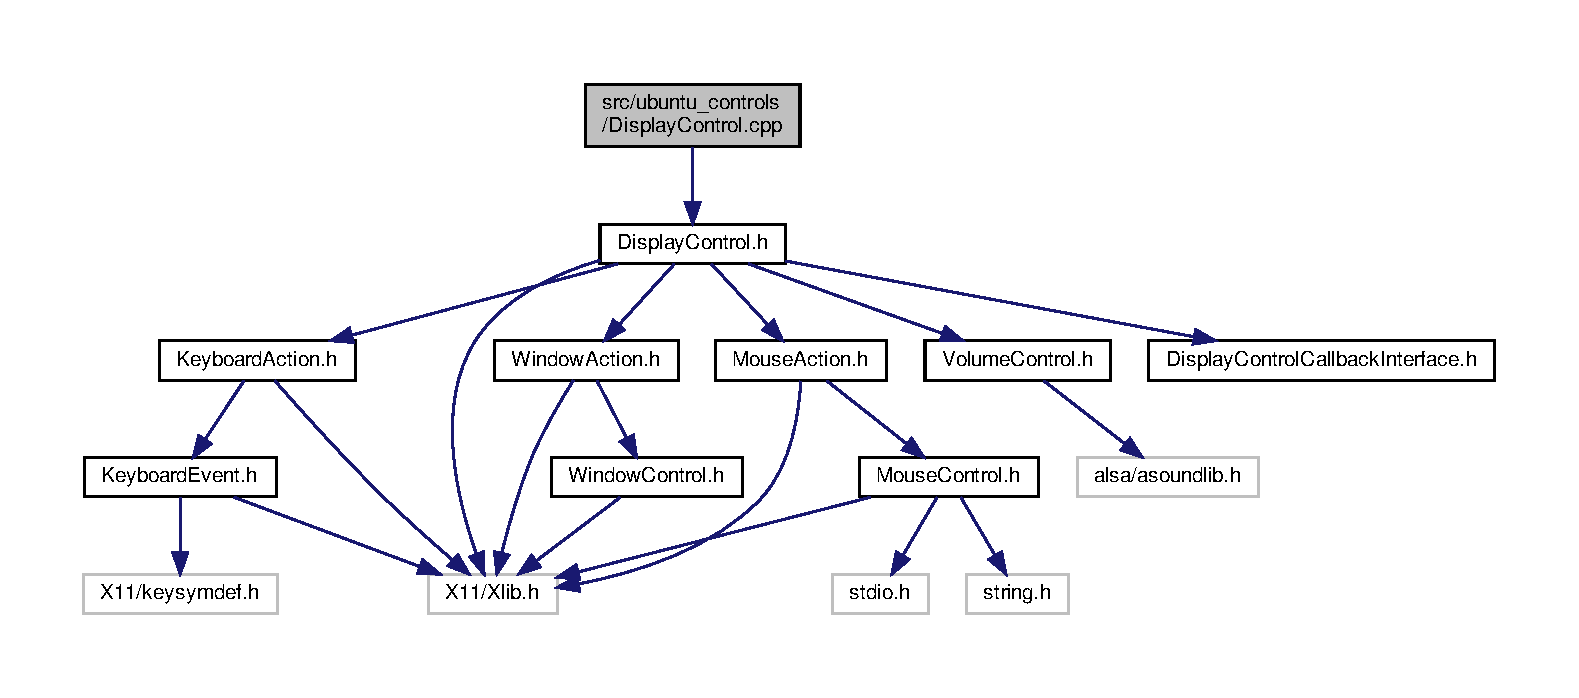
\includegraphics[width=350pt]{DisplayControl_8cpp__incl}
\end{center}
\end{figure}

\hypertarget{DisplayControl_8h}{}\section{src/ubuntu\+\_\+controls/\+Display\+Control.h File Reference}
\label{DisplayControl_8h}\index{src/ubuntu\+\_\+controls/\+Display\+Control.\+h@{src/ubuntu\+\_\+controls/\+Display\+Control.\+h}}
{\ttfamily \#include \char`\"{}Window\+Action.\+h\char`\"{}}\newline
{\ttfamily \#include \char`\"{}Keyboard\+Action.\+h\char`\"{}}\newline
{\ttfamily \#include \char`\"{}Volume\+Control.\+h\char`\"{}}\newline
{\ttfamily \#include \char`\"{}Mouse\+Action.\+h\char`\"{}}\newline
{\ttfamily \#include \char`\"{}Display\+Control\+Callback\+Interface.\+h\char`\"{}}\newline
{\ttfamily \#include $<$X11/\+Xlib.\+h$>$}\newline
Include dependency graph for Display\+Control.\+h\+:\nopagebreak
\begin{figure}[H]
\begin{center}
\leavevmode
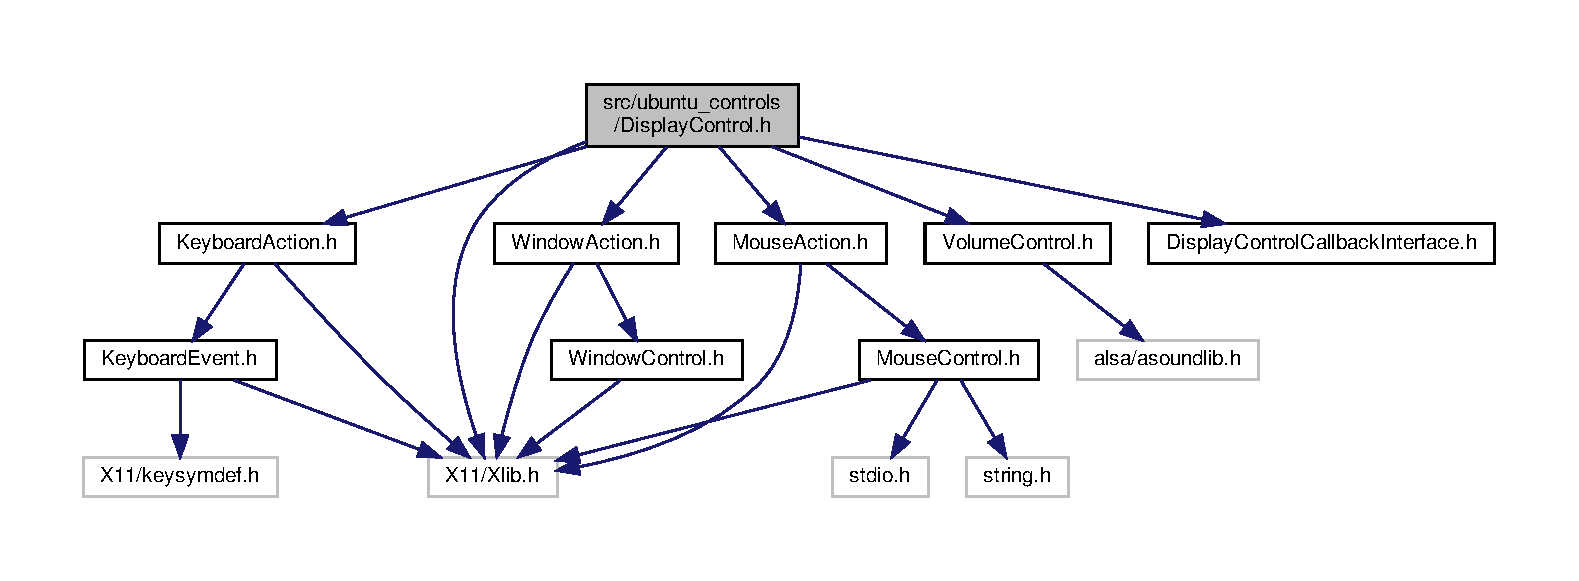
\includegraphics[width=350pt]{DisplayControl_8h__incl}
\end{center}
\end{figure}
This graph shows which files directly or indirectly include this file\+:\nopagebreak
\begin{figure}[H]
\begin{center}
\leavevmode
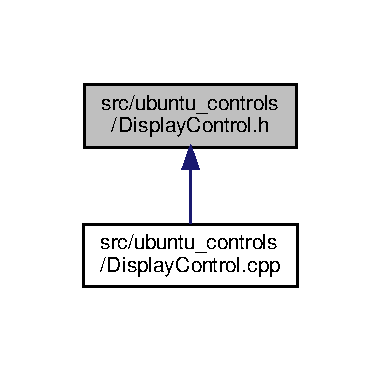
\includegraphics[width=183pt]{DisplayControl_8h__dep__incl}
\end{center}
\end{figure}
\subsection*{Classes}
\begin{DoxyCompactItemize}
\item 
class \hyperlink{classGestro_1_1DisplayControl}{Gestro\+::\+Display\+Control}
\begin{DoxyCompactList}\small\item\em This is a class that is inheriting from the classes Window\+Action, Keyboard\+Action, Mouse\+Action, Volume\+Control, and \hyperlink{classGestro_1_1DisplayControlCallbackInterface}{Display\+Control\+Callback\+Interface}. \end{DoxyCompactList}\end{DoxyCompactItemize}
\subsection*{Namespaces}
\begin{DoxyCompactItemize}
\item 
 \hyperlink{namespaceGestro}{Gestro}
\end{DoxyCompactItemize}

\hypertarget{DisplayControlCallbackInterface_8h}{}\section{src/ubuntu\+\_\+controls/\+Display\+Control\+Callback\+Interface.h File Reference}
\label{DisplayControlCallbackInterface_8h}\index{src/ubuntu\+\_\+controls/\+Display\+Control\+Callback\+Interface.\+h@{src/ubuntu\+\_\+controls/\+Display\+Control\+Callback\+Interface.\+h}}
This graph shows which files directly or indirectly include this file\+:\nopagebreak
\begin{figure}[H]
\begin{center}
\leavevmode
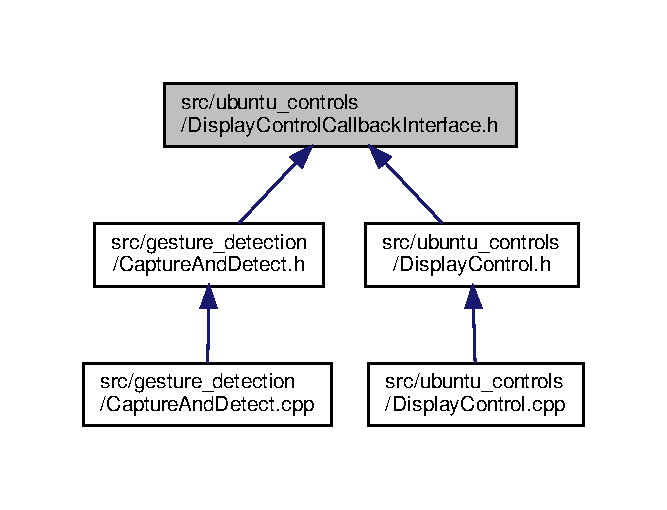
\includegraphics[width=320pt]{DisplayControlCallbackInterface_8h__dep__incl}
\end{center}
\end{figure}
\subsection*{Classes}
\begin{DoxyCompactItemize}
\item 
class \hyperlink{classGestro_1_1DisplayControlCallbackInterface}{Gestro\+::\+Display\+Control\+Callback\+Interface}
\end{DoxyCompactItemize}
\subsection*{Namespaces}
\begin{DoxyCompactItemize}
\item 
 \hyperlink{namespaceGestro}{Gestro}
\end{DoxyCompactItemize}

\hypertarget{KeyboardAction_8cpp}{}\section{src/ubuntu\+\_\+controls/\+Keyboard\+Action.cpp File Reference}
\label{KeyboardAction_8cpp}\index{src/ubuntu\+\_\+controls/\+Keyboard\+Action.\+cpp@{src/ubuntu\+\_\+controls/\+Keyboard\+Action.\+cpp}}
{\ttfamily \#include \char`\"{}Keyboard\+Action.\+h\char`\"{}}\newline
Include dependency graph for Keyboard\+Action.\+cpp\+:\nopagebreak
\begin{figure}[H]
\begin{center}
\leavevmode
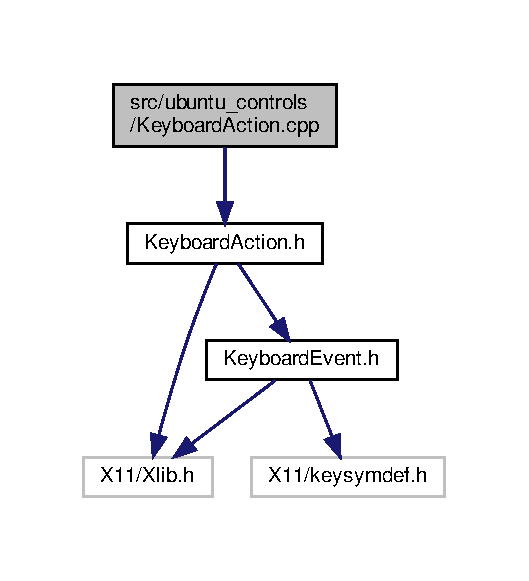
\includegraphics[width=254pt]{KeyboardAction_8cpp__incl}
\end{center}
\end{figure}

\hypertarget{KeyboardAction_8h}{}\section{src/ubuntu\+\_\+controls/\+Keyboard\+Action.h File Reference}
\label{KeyboardAction_8h}\index{src/ubuntu\+\_\+controls/\+Keyboard\+Action.\+h@{src/ubuntu\+\_\+controls/\+Keyboard\+Action.\+h}}
{\ttfamily \#include $<$X11/\+Xlib.\+h$>$}\newline
{\ttfamily \#include \char`\"{}Keyboard\+Event.\+h\char`\"{}}\newline
Include dependency graph for Keyboard\+Action.\+h\+:\nopagebreak
\begin{figure}[H]
\begin{center}
\leavevmode
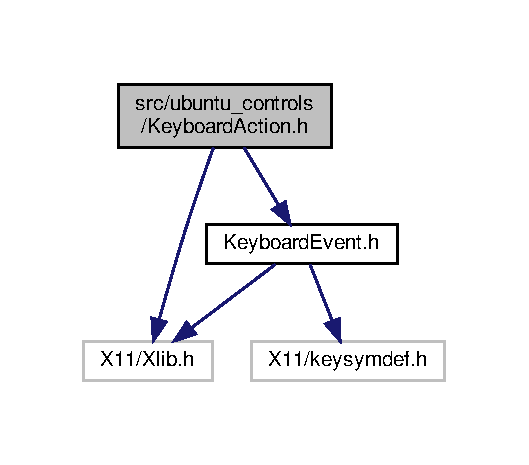
\includegraphics[width=254pt]{KeyboardAction_8h__incl}
\end{center}
\end{figure}
This graph shows which files directly or indirectly include this file\+:\nopagebreak
\begin{figure}[H]
\begin{center}
\leavevmode
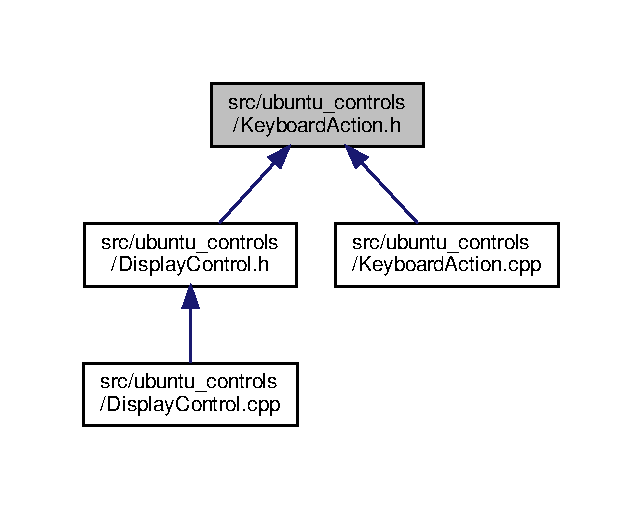
\includegraphics[width=308pt]{KeyboardAction_8h__dep__incl}
\end{center}
\end{figure}
\subsection*{Classes}
\begin{DoxyCompactItemize}
\item 
class \hyperlink{classUbuntuController_1_1KeyboardAction}{Ubuntu\+Controller\+::\+Keyboard\+Action}
\begin{DoxyCompactList}\small\item\em A wrapper class for Keyboard Event. \end{DoxyCompactList}\end{DoxyCompactItemize}
\subsection*{Namespaces}
\begin{DoxyCompactItemize}
\item 
 \hyperlink{namespaceUbuntuController}{Ubuntu\+Controller}
\end{DoxyCompactItemize}

\hypertarget{KeyboardEvent_8cpp}{}\section{src/ubuntu\+\_\+controls/\+Keyboard\+Event.cpp File Reference}
\label{KeyboardEvent_8cpp}\index{src/ubuntu\+\_\+controls/\+Keyboard\+Event.\+cpp@{src/ubuntu\+\_\+controls/\+Keyboard\+Event.\+cpp}}
{\ttfamily \#include \char`\"{}Keyboard\+Event.\+h\char`\"{}}\newline
Include dependency graph for Keyboard\+Event.\+cpp\+:\nopagebreak
\begin{figure}[H]
\begin{center}
\leavevmode
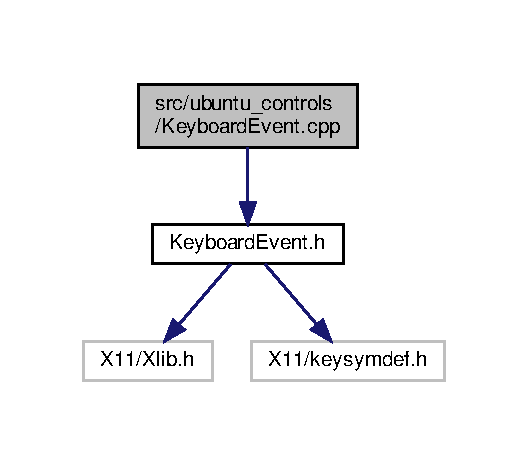
\includegraphics[width=254pt]{KeyboardEvent_8cpp__incl}
\end{center}
\end{figure}

\hypertarget{KeyboardEvent_8h}{}\section{src/ubuntu\+\_\+controls/\+Keyboard\+Event.h File Reference}
\label{KeyboardEvent_8h}\index{src/ubuntu\+\_\+controls/\+Keyboard\+Event.\+h@{src/ubuntu\+\_\+controls/\+Keyboard\+Event.\+h}}
{\ttfamily \#include $<$X11/\+Xlib.\+h$>$}\newline
{\ttfamily \#include $<$X11/keysymdef.\+h$>$}\newline
Include dependency graph for Keyboard\+Event.\+h\+:\nopagebreak
\begin{figure}[H]
\begin{center}
\leavevmode
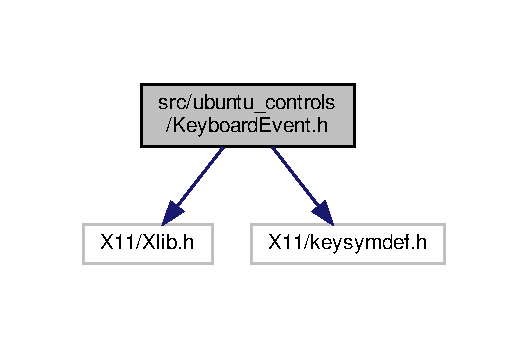
\includegraphics[width=254pt]{KeyboardEvent_8h__incl}
\end{center}
\end{figure}
This graph shows which files directly or indirectly include this file\+:\nopagebreak
\begin{figure}[H]
\begin{center}
\leavevmode
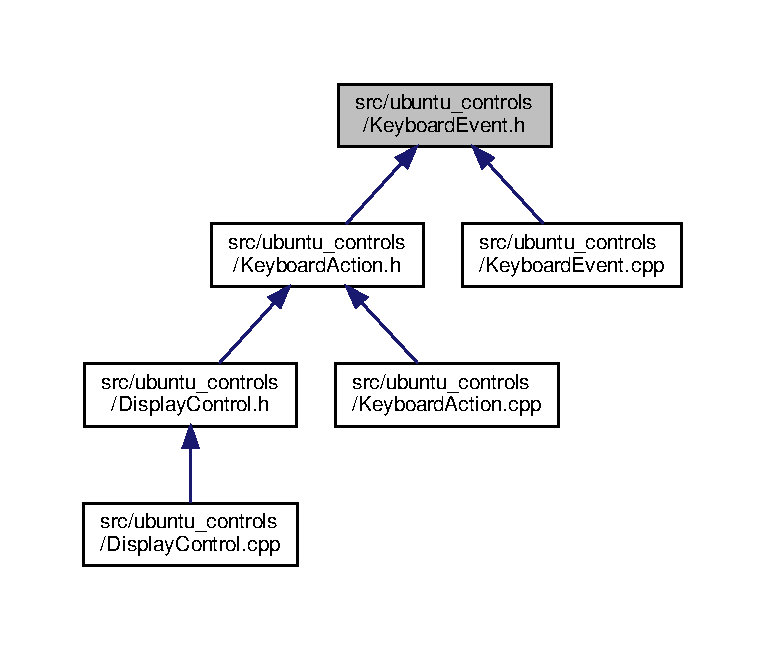
\includegraphics[width=350pt]{KeyboardEvent_8h__dep__incl}
\end{center}
\end{figure}
\subsection*{Classes}
\begin{DoxyCompactItemize}
\item 
class \hyperlink{classUbuntuController_1_1KeyboardEvent}{Ubuntu\+Controller\+::\+Keyboard\+Event}
\begin{DoxyCompactList}\small\item\em Used to send keyboard events. \end{DoxyCompactList}\end{DoxyCompactItemize}
\subsection*{Namespaces}
\begin{DoxyCompactItemize}
\item 
 \hyperlink{namespaceUbuntuController}{Ubuntu\+Controller}
\end{DoxyCompactItemize}

\hypertarget{MouseAction_8cpp}{}\section{src/ubuntu\+\_\+controls/\+Mouse\+Action.cpp File Reference}
\label{MouseAction_8cpp}\index{src/ubuntu\+\_\+controls/\+Mouse\+Action.\+cpp@{src/ubuntu\+\_\+controls/\+Mouse\+Action.\+cpp}}
{\ttfamily \#include \char`\"{}Mouse\+Action.\+h\char`\"{}}\newline
Include dependency graph for Mouse\+Action.\+cpp\+:\nopagebreak
\begin{figure}[H]
\begin{center}
\leavevmode
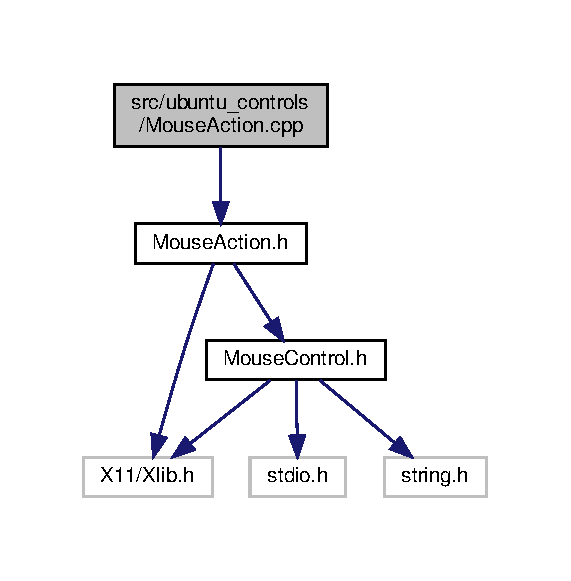
\includegraphics[width=274pt]{MouseAction_8cpp__incl}
\end{center}
\end{figure}

\hypertarget{MouseAction_8h}{}\section{src/ubuntu\+\_\+controls/\+Mouse\+Action.h File Reference}
\label{MouseAction_8h}\index{src/ubuntu\+\_\+controls/\+Mouse\+Action.\+h@{src/ubuntu\+\_\+controls/\+Mouse\+Action.\+h}}
{\ttfamily \#include $<$X11/\+Xlib.\+h$>$}\newline
{\ttfamily \#include \char`\"{}Mouse\+Control.\+h\char`\"{}}\newline
Include dependency graph for Mouse\+Action.\+h\+:\nopagebreak
\begin{figure}[H]
\begin{center}
\leavevmode
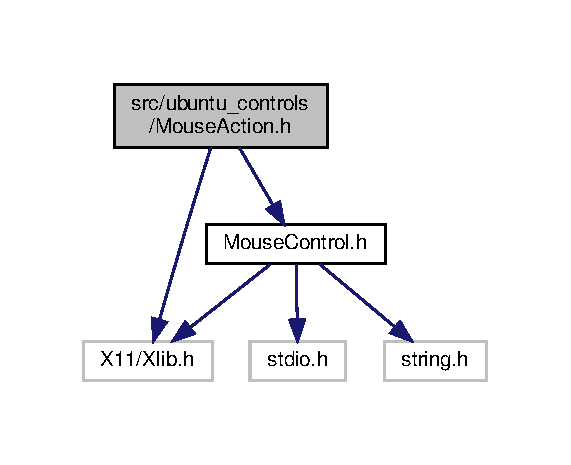
\includegraphics[width=274pt]{MouseAction_8h__incl}
\end{center}
\end{figure}
This graph shows which files directly or indirectly include this file\+:\nopagebreak
\begin{figure}[H]
\begin{center}
\leavevmode
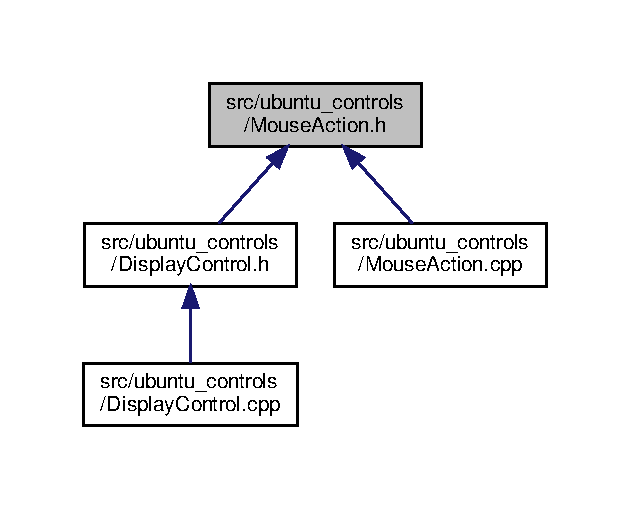
\includegraphics[width=303pt]{MouseAction_8h__dep__incl}
\end{center}
\end{figure}
\subsection*{Classes}
\begin{DoxyCompactItemize}
\item 
class \hyperlink{classUbuntuController_1_1MouseAction}{Ubuntu\+Controller\+::\+Mouse\+Action}
\begin{DoxyCompactList}\small\item\em A wrapper class for mouse control. \end{DoxyCompactList}\end{DoxyCompactItemize}
\subsection*{Namespaces}
\begin{DoxyCompactItemize}
\item 
 \hyperlink{namespaceUbuntuController}{Ubuntu\+Controller}
\end{DoxyCompactItemize}

\hypertarget{MouseControl_8cpp}{}\section{src/ubuntu\+\_\+controls/\+Mouse\+Control.cpp File Reference}
\label{MouseControl_8cpp}\index{src/ubuntu\+\_\+controls/\+Mouse\+Control.\+cpp@{src/ubuntu\+\_\+controls/\+Mouse\+Control.\+cpp}}
{\ttfamily \#include \char`\"{}Mouse\+Control.\+h\char`\"{}}\newline
Include dependency graph for Mouse\+Control.\+cpp\+:\nopagebreak
\begin{figure}[H]
\begin{center}
\leavevmode
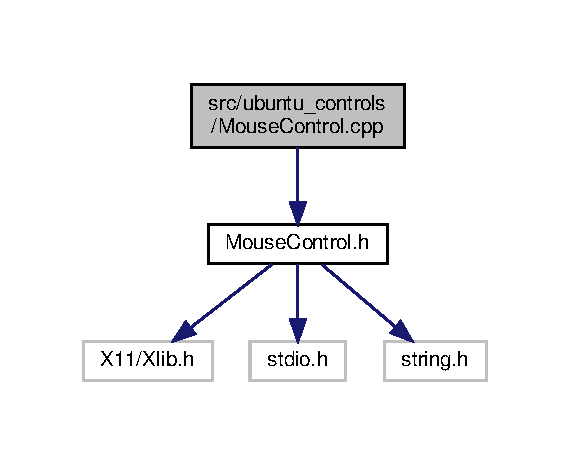
\includegraphics[width=274pt]{MouseControl_8cpp__incl}
\end{center}
\end{figure}

\hypertarget{MouseControl_8h}{}\section{src/ubuntu\+\_\+controls/\+Mouse\+Control.h File Reference}
\label{MouseControl_8h}\index{src/ubuntu\+\_\+controls/\+Mouse\+Control.\+h@{src/ubuntu\+\_\+controls/\+Mouse\+Control.\+h}}
{\ttfamily \#include $<$X11/\+Xlib.\+h$>$}\newline
{\ttfamily \#include $<$stdio.\+h$>$}\newline
{\ttfamily \#include $<$string.\+h$>$}\newline
Include dependency graph for Mouse\+Control.\+h\+:\nopagebreak
\begin{figure}[H]
\begin{center}
\leavevmode
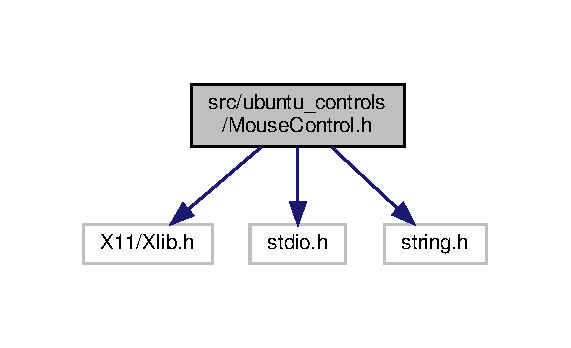
\includegraphics[width=274pt]{MouseControl_8h__incl}
\end{center}
\end{figure}
This graph shows which files directly or indirectly include this file\+:\nopagebreak
\begin{figure}[H]
\begin{center}
\leavevmode
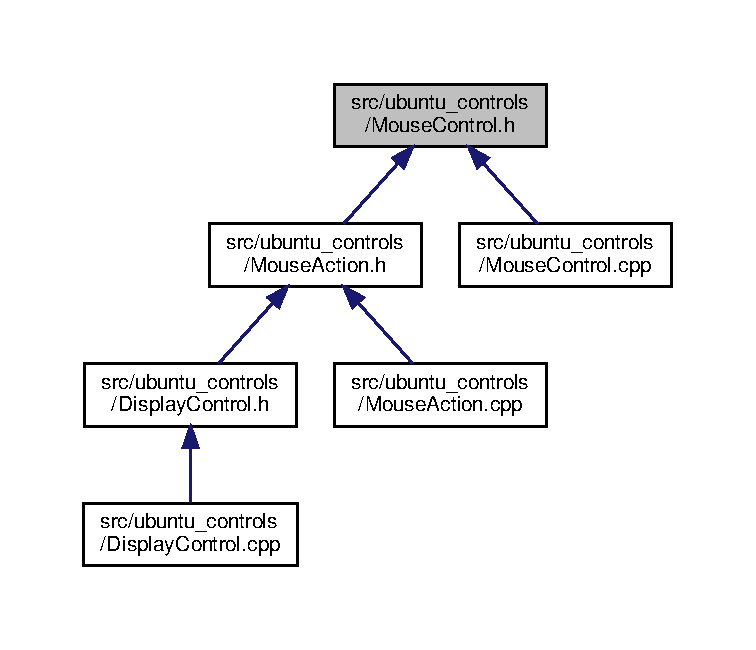
\includegraphics[width=350pt]{MouseControl_8h__dep__incl}
\end{center}
\end{figure}
\subsection*{Classes}
\begin{DoxyCompactItemize}
\item 
class \hyperlink{classUbuntuController_1_1MouseControl}{Ubuntu\+Controller\+::\+Mouse\+Control}
\begin{DoxyCompactList}\small\item\em Used to send mouse events. \end{DoxyCompactList}\end{DoxyCompactItemize}
\subsection*{Namespaces}
\begin{DoxyCompactItemize}
\item 
 \hyperlink{namespaceUbuntuController}{Ubuntu\+Controller}
\end{DoxyCompactItemize}

\hypertarget{VolumeControl_8cpp}{}\section{src/ubuntu\+\_\+controls/\+Volume\+Control.cpp File Reference}
\label{VolumeControl_8cpp}\index{src/ubuntu\+\_\+controls/\+Volume\+Control.\+cpp@{src/ubuntu\+\_\+controls/\+Volume\+Control.\+cpp}}
{\ttfamily \#include \char`\"{}Volume\+Control.\+h\char`\"{}}\newline
{\ttfamily \#include \char`\"{}iostream\char`\"{}}\newline
{\ttfamily \#include \char`\"{}stdio.\+h\char`\"{}}\newline
Include dependency graph for Volume\+Control.\+cpp\+:\nopagebreak
\begin{figure}[H]
\begin{center}
\leavevmode
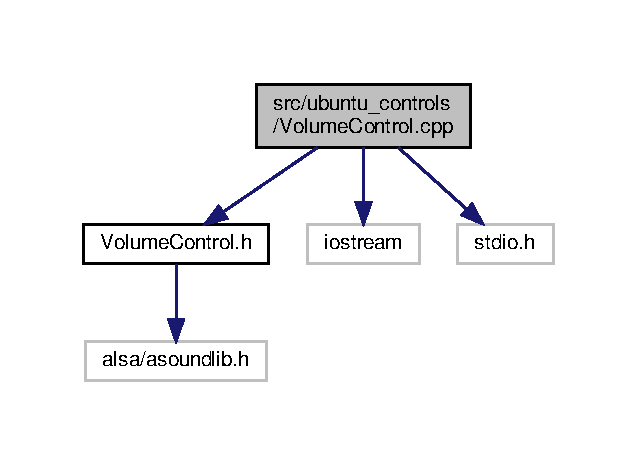
\includegraphics[width=306pt]{VolumeControl_8cpp__incl}
\end{center}
\end{figure}

\hypertarget{VolumeControl_8h}{}\section{src/ubuntu\+\_\+controls/\+Volume\+Control.h File Reference}
\label{VolumeControl_8h}\index{src/ubuntu\+\_\+controls/\+Volume\+Control.\+h@{src/ubuntu\+\_\+controls/\+Volume\+Control.\+h}}
{\ttfamily \#include $<$alsa/asoundlib.\+h$>$}\newline
Include dependency graph for Volume\+Control.\+h\+:\nopagebreak
\begin{figure}[H]
\begin{center}
\leavevmode
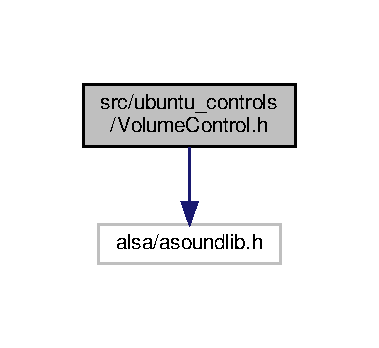
\includegraphics[width=182pt]{VolumeControl_8h__incl}
\end{center}
\end{figure}
This graph shows which files directly or indirectly include this file\+:\nopagebreak
\begin{figure}[H]
\begin{center}
\leavevmode
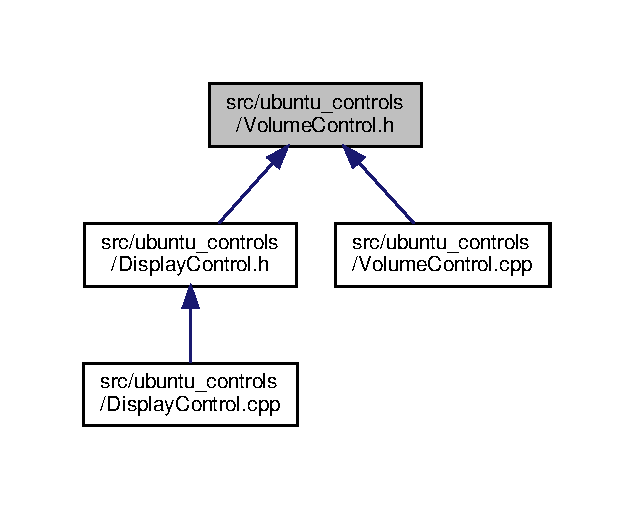
\includegraphics[width=304pt]{VolumeControl_8h__dep__incl}
\end{center}
\end{figure}
\subsection*{Classes}
\begin{DoxyCompactItemize}
\item 
class \hyperlink{classUbuntuController_1_1VolumeControl}{Ubuntu\+Controller\+::\+Volume\+Control}
\begin{DoxyCompactList}\small\item\em This class uses the A\+L\+SA library to send commands to the sound card. \end{DoxyCompactList}\end{DoxyCompactItemize}
\subsection*{Namespaces}
\begin{DoxyCompactItemize}
\item 
 \hyperlink{namespaceUbuntuController}{Ubuntu\+Controller}
\end{DoxyCompactItemize}

\hypertarget{WindowAction_8cpp}{}\section{src/ubuntu\+\_\+controls/\+Window\+Action.cpp File Reference}
\label{WindowAction_8cpp}\index{src/ubuntu\+\_\+controls/\+Window\+Action.\+cpp@{src/ubuntu\+\_\+controls/\+Window\+Action.\+cpp}}
{\ttfamily \#include \char`\"{}Window\+Action.\+h\char`\"{}}\newline
Include dependency graph for Window\+Action.\+cpp\+:\nopagebreak
\begin{figure}[H]
\begin{center}
\leavevmode
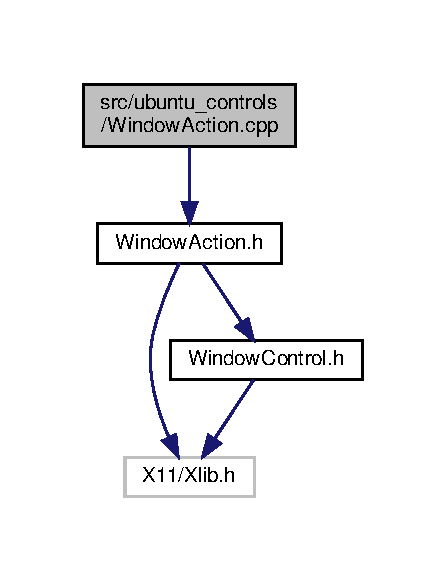
\includegraphics[width=214pt]{WindowAction_8cpp__incl}
\end{center}
\end{figure}

\hypertarget{WindowAction_8h}{}\section{src/ubuntu\+\_\+controls/\+Window\+Action.h File Reference}
\label{WindowAction_8h}\index{src/ubuntu\+\_\+controls/\+Window\+Action.\+h@{src/ubuntu\+\_\+controls/\+Window\+Action.\+h}}
{\ttfamily \#include $<$X11/\+Xlib.\+h$>$}\newline
{\ttfamily \#include \char`\"{}Window\+Control.\+h\char`\"{}}\newline
Include dependency graph for Window\+Action.\+h\+:\nopagebreak
\begin{figure}[H]
\begin{center}
\leavevmode
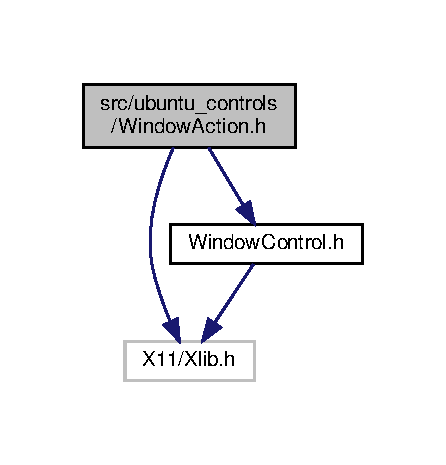
\includegraphics[width=214pt]{WindowAction_8h__incl}
\end{center}
\end{figure}
This graph shows which files directly or indirectly include this file\+:\nopagebreak
\begin{figure}[H]
\begin{center}
\leavevmode
\includegraphics[width=303pt]{WindowAction_8h__dep__incl}
\end{center}
\end{figure}
\subsection*{Classes}
\begin{DoxyCompactItemize}
\item 
class \hyperlink{classUbuntuController_1_1WindowAction}{Ubuntu\+Controller\+::\+Window\+Action}
\begin{DoxyCompactList}\small\item\em Contains functions that accessed by Display\+Control to access the \hyperlink{classUbuntuController_1_1WindowControl}{Window\+Control}. \end{DoxyCompactList}\end{DoxyCompactItemize}
\subsection*{Namespaces}
\begin{DoxyCompactItemize}
\item 
 \hyperlink{namespaceUbuntuController}{Ubuntu\+Controller}
\end{DoxyCompactItemize}

\hypertarget{WindowControl_8cpp}{}\section{src/ubuntu\+\_\+controls/\+Window\+Control.cpp File Reference}
\label{WindowControl_8cpp}\index{src/ubuntu\+\_\+controls/\+Window\+Control.\+cpp@{src/ubuntu\+\_\+controls/\+Window\+Control.\+cpp}}
{\ttfamily \#include \char`\"{}Window\+Control.\+h\char`\"{}}\newline
{\ttfamily \#include \char`\"{}iostream\char`\"{}}\newline
Include dependency graph for Window\+Control.\+cpp\+:\nopagebreak
\begin{figure}[H]
\begin{center}
\leavevmode
\includegraphics[width=244pt]{WindowControl_8cpp__incl}
\end{center}
\end{figure}

\hypertarget{WindowControl_8h}{}\section{src/ubuntu\+\_\+controls/\+Window\+Control.h File Reference}
\label{WindowControl_8h}\index{src/ubuntu\+\_\+controls/\+Window\+Control.\+h@{src/ubuntu\+\_\+controls/\+Window\+Control.\+h}}
{\ttfamily \#include $<$X11/\+Xlib.\+h$>$}\newline
Include dependency graph for Window\+Control.\+h\+:\nopagebreak
\begin{figure}[H]
\begin{center}
\leavevmode
\includegraphics[width=182pt]{WindowControl_8h__incl}
\end{center}
\end{figure}
This graph shows which files directly or indirectly include this file\+:\nopagebreak
\begin{figure}[H]
\begin{center}
\leavevmode
\includegraphics[width=350pt]{WindowControl_8h__dep__incl}
\end{center}
\end{figure}
\subsection*{Classes}
\begin{DoxyCompactItemize}
\item 
class \hyperlink{classWindowControl}{Window\+Control}
\begin{DoxyCompactList}\small\item\em Used to send window events. \end{DoxyCompactList}\end{DoxyCompactItemize}

%--- End generated contents ---

% Index
\backmatter
\newpage
\phantomsection
\clearemptydoublepage
\addcontentsline{toc}{chapter}{Index}
\printindex

\end{document}
